\documentclass[a4paper,11pt,twoside]{report}

% ============================================
% ===== PREÁMBULO - PAQUETES ORDENADOS =====
% ============================================

% 1. ENCODING Y LENGUAJE (siempre primero)
\usepackage[utf8]{inputenc}
\usepackage[T1]{fontenc}
\usepackage[spanish]{babel}

% 2. FORMATO DE TEXTO Y PÁGINA
\usepackage{indentfirst}          % Sangría en primer párrafo
\usepackage{setspace}             % Control de interlineado
\usepackage{soul}                 % Texto tachado (\st{})
\usepackage{paralist}             % Listas compactas
\usepackage{nameref}              % Referencias por nombre
\usepackage{verbatim}             % Texto verbatim


% 3. CONFIGURACIÓN DE PÁGINA (GEOMETRÍA)
% ¡SOLO UNA configuración de geometry! Elijo la segunda que tenías
\usepackage[top=3cm,bottom=4cm,left=2cm,right=2.5cm,twoside]{geometry}
\setlength{\headheight}{15pt}
\addtolength{\topmargin}{-3pt}

% 4. GRÁFICOS Y COLORES
\usepackage{graphicx}                        % Incluir imágenes
\usepackage[table,dvipsnames]{xcolor}        % Colores en tablas
\usepackage{tikz}                            % Gráficos vectoriales
\usepackage{tcolorbox}                       % Cajas con color
\usetikzlibrary{shapes, arrows, positioning} %librerias de tikz

% 5. TABLAS
\usepackage{float}                % Posicionamiento de tablas
\usepackage{booktabs}             % Líneas profesionales en tablas
\usepackage{multirow}             % Multiples filas en tablas
\usepackage{caption}              % Personalización de leyendas
\captionsetup[table]{name=Tabla}  % Cambiar "Table" por "Tabla"

% 6. MATEMÁTICAS
\usepackage{amsmath}              % Símbolos y entornos matemáticos
\usepackage{amssymb}              % Símbolos matemáticos adicionales

% 7. CÓDIGO FUENTE
\usepackage{listings}             % Incluir código
\usepackage{upquote}              % Comillas rectas en lstlisting
\usepackage{xcolor}               % Colores para el código (ya cargado)

% 8. REFERENCIAS Y ENLACES
\usepackage{hyperref}             % Enlaces en el documento


% 9. ENCABEZADOS Y FORMATO DE CAPÍTULOS
\usepackage{fancyhdr}             % Encabezados y pies personalizados
\usepackage{titlesec}             % Formato de títulos de secciones
\usepackage{etoolbox}             % Utilidades para capítulos

% 10. Para hacer listas dentro de listas numeradas
%\usepackage{enumitem}
\usepackage{pdflscape}
\usepackage{tabularx}
\usepackage{colortbl}
\usepackage{xcolor}
\usepackage{array}

% 10. BIBLIOGRAFÍA
\usepackage{csquotes}
\usepackage[
  backend=biber,
  style=ieee,           
  url=true,
  urldate=iso,
  seconds=true
]{biblatex}
\addbibresource{bibliografia.bib}

% 11. Configuración para JSON
\lstdefinelanguage{json}{
    keywords={true,false,null},
    keywordstyle=\color{blue}\bfseries,
    ndkeywords={products,meterId,meterDesc,deprecated,unit,type,unitCost,quantity},
    ndkeywordstyle=\color{purple}\bfseries,
    identifierstyle=\color{black},
    sensitive=false,
    comment=[l]{//},
    morecomment=[s]{/*}{*/},
    commentstyle=\color{gray}\ttfamily,
    stringstyle=\color{teal}\ttfamily,
    morestring=[b]",
    morestring=[b]'
}

\lstset{
    language=json,
    basicstyle=\ttfamily\small,
    numbers=left,
    numberstyle=\tiny\color{gray},
    stepnumber=1,
    numbersep=5pt,
    backgroundcolor=\color{gray!10},
    showspaces=false,
    showstringspaces=false,
    showtabs=false,
    frame=single,
    rulecolor=\color{black!30},
    tabsize=2,
    captionpos=b,
    breaklines=true,
    breakatwhitespace=true,
    title=\lstname,
    escapeinside={\%*}{*)},
    literate={\ \ }{{\ }}1
}
% Para cambiar el formato de \paragraph
\titleformat{\paragraph}
  {\normalfont\bfseries}           % Formato del título
  {\theparagraph}                   % Numeración
  {1em}                             % Espacio entre número y título
  {}                                % Código antes del título
  [\vspace{0.5ex}]                  % Código después del título (salto de línea)

\titlespacing*{\paragraph}
  {0pt}                             % Margen izquierdo
  {3.25ex plus 1ex minus 0.2ex}     % Espacio antes
  {0.5em}                           % Espacio después
% A. Configuración de hyperref (DEBE ir después de cargar hyperref)
\hypersetup{
    colorlinks=true,
    linkcolor=blue,
    citecolor=green,
    filecolor=magenta,      
    urlcolor=cyan,
    pdfauthor={Pablo Galilea Valverde},
    pdftitle={Trabajo Fin de Grado: Sistema de gestión de automatización de test},
    pdfsubject={Trabajo Fin de Grado en Ingeniería Informática},
    pdfkeywords={automatización, testing, sistemas de negocio, hosting}
}

% B. Configuración de encabezados (fancyhdr)
\pagestyle{fancy}
\fancyhf{}  % Limpiar encabezados y pies
\fancyhead[LE,RO]{\thepage}     % Número de página exterior
\fancyhead[RE]{\leftmark}       % Nombre del capítulo (páginas pares)
\fancyhead[LO]{\rightmark}      % Nombre de sección (páginas impares)

% C. Configuración de formato de capítulos (titlesec)
\titleformat{\chapter}[display]
  {\normalfont\huge\bfseries\centering}
  {\chaptertitlename\ \thechapter}
  {20pt}
  {\Huge}
\titlespacing*{\chapter}{0pt}{-30pt}{20pt}  % Ajuste de espacios

% D. Configuración para capítulos en la misma página (etoolbox)
\makeatletter
\patchcmd{\chapter}{\if@openright\cleardoublepage\else\clearpage\fi}{}{}{}
\makeatother

% E. Configuración de listings (código fuente)
\lstset{
    basicstyle=\ttfamily\small,
    keywordstyle=\color{blue},
    commentstyle=\color{gray},
    numbers=left,
    numberstyle=\tiny\color{gray},
    frame=single,
    breaklines=true,
    showstringspaces=false
}

% F. Configuración de gráficos (ruta de imágenes)
\graphicspath{ {./imagenes/} }  % Carpeta donde buscar imágenes

% G. Otros ajustes
\setlength{\arrayrulewidth}{0.5pt}  % Grosor de líneas en tablas
\setlength{\tabcolsep}{12pt}        % Espacio en celdas de tabla
\renewcommand{\arraystretch}{1.2}   % Altura de filas en tablas

%\setlist[enumerate,1]{label=\arabic*., ref=\arabic*}
%\setlist[enumerate,2]{label=\arabic*.\arabic*., ref=\arabic*.\arabic*, resume}
%\setlist[enumerate,3]{label=\arabic*.\arabic*.\arabic*., ref=\arabic*.\arabic*.\arabic*, resume}

\sloppy  % Evita errores de desbordamiento de línea

% ============================================
% ===== METADATOS DEL DOCUMENTO =====
% ============================================

\title{Sistema de gestión de automatización de test para los sistemas de negocio de una compañía de hosting}
\author{Pablo Galilea Valverde}
\date{Junio 2025}


% ============================================
% ===== CUERPO DEL DOCUMENTO =====
% ============================================

% ===== DOCUMENTO =====
\begin{document}

% Portada
%PORTADA
\begin{titlepage}
    \begin{center}
        \vspace*{-1in}
        \begin{figure}[htb]
            \begin{center}
                \vspace*{0.3in}
                
\includegraphics[width=6.5cm]{./imagenes/logo.jpg}
                %\caption*{}
            \end{center}
        \end{figure}
        \begin{Large}
            \textbf{Facultad de Ciencia y Tecnología\\}
        \end{Large}
        \vspace*{0.5in}
        \begin{Huge}
            \textbf{TRABAJO FIN DE GRADO}\\
        \end{Huge}
        \vspace*{0.16in}
        \begin{huge}
            \textbf{Grado en Ingeniería Informática \\}
        \end{huge}

        \vspace*{0.3in}
        \begin{tcolorbox}[colback=white]
            \begin{Huge}
                \begin{center}
                    \textbf{Sistema de Validación en Facturación de Servicios Cloud}
                \end{center}
            \end{Huge}
        \end{tcolorbox}

        \begin{tcolorbox}[colback=white]
            \begin{Huge}
                \begin{center}
                    \textbf{Cloud Services Billing Validation System}
                \end{center}
            \end{Huge}
        \end{tcolorbox}

        \vspace*{0.2in}
        \begin{large}
            Realizado por:\\
        \end{large}
        \vspace*{0.1in}
        \begin{Large}
            \textbf{Pablo Galilea Valverde\\}
        \end{Large}
        \vspace*{0.2in}
        \begin{large}
            Tutelado por:\\
        \end{large}
        \vspace*{0.1in}

        \begin{Large}
            \textbf{Jesús María Aransay Azofra\\}
        \end{Large}

        \vspace*{0.8in}
        \textbf{Logroño, Curso 2025-2026}

    \end{center}

\end{titlepage}


% ===== PÁGINA DE DEDICATORIA (OPCIONAL) =====
% Si NO quieres página en blanco, usa esto:
\clearpage  % En lugar de \cleardoublepage
\thispagestyle{empty}
\begin{center}
  \vspace*{5cm}  % Espacio vertical

  \textit{Dedicado a...}

  \vspace{2cm}

  \textit{A mis padres y mi hermano por su apoyo incondicional.} \\ % 

  \vspace{2cm}   % Espacio final
\end{center}
\clearpage  % Pasa a la siguiente página

% ===== PÁGINAS PRELIMINARES =====
% Configurar numeración romana para preliminares
\pagenumbering{roman}
\setcounter{page}{3}  % Empezar en página iii (portada = i, dedicatoria = ii)

% ===== RESUMEN =====
\chapter*{Resumen}
\thispagestyle{empty}  % Sin número en primera página del resumen
\addcontentsline{toc}{chapter}{Resumen}  % Añadir al índice

\textbf{Palabras clave:} automatización, testing, facturación, nube, validación, Node.js, CouchDB.

\vspace{0.5cm}

Este proyecto desarrolla un sistema automatizado de validación de la facturación del DCD (\textit{Data Center Designer}) de IONOS Cloud. El problema de partida es que, con decenas de SKUs facturables y múltiples tipos de recursos, verificar manualmente la corrección de los cargos resulta inviable a escala. La solución consiste en un servicio construido en Node.js que orquesta dos tipos de comprobación: por un lado, verifica que los recursos de consumo constante —máquinas virtuales, almacenamiento y discos— figuran correctamente en la factura mensual; por otro, genera y valida consumo variable artificial —llamadas DNS, tokens de inteligencia artificial— asegurando que las cantidades facturadas coinciden con las esperadas dentro de márgenes configurables por SKU.

El sistema se apoya en CouchDB para almacenar la configuración y el histórico de verificaciones, y emplea jobs cron para programar las comprobaciones periódicas. Ante cualquier desviación significativa, lanza notificaciones automáticas al equipo. El desarrollo se llevó a cabo en cinco iteraciones siguiendo una metodología ágil, logrando cubrir la totalidad de los requisitos funcionales y no funcionales con una desviación respecto a la planificación inferior al 3\%.

\vspace{2cm}

% ===== ABSTRACT =====
\chapter*{Abstract}
\thispagestyle{empty}
\addcontentsline{toc}{chapter}{Abstract}

\textbf{Keywords:} automation, testing, billing, cloud, validation, Node.js, CouchDB.

\vspace{0.5cm}

This project develops an automated billing validation system for the IONOS Cloud DCD (\textit{Data Center Designer}). Given the scale of the platform — with dozens of billable SKUs and multiple resource types — manual verification of billing accuracy is not feasible. The solution is a Node.js service that orchestrates two complementary validation flows: first, it checks that continuously consumed resources — virtual machines, object storage, and block disks — are correctly reflected in the monthly invoice; second, it generates and validates artificial variable consumption — DNS queries, AI token usage — verifying that the billed amounts match the expected values within per-SKU configurable tolerance margins.

CouchDB is used to store configuration and the historical log of verifications, while cron jobs drive the periodic execution schedule. Any significant deviation triggers automatic notifications to the team. The system was built across five agile iterations, achieving full coverage of all functional and non-functional requirements with a total schedule deviation of under 3\%.

\vspace{2cm}

\newpage

% ===== AGRADECIMIENTOS =====
\chapter*{Agradecimientos}
\thispagestyle{empty}
\addcontentsline{toc}{chapter}{Agradecimientos}

En primer lugar, me gustaría expresar mi más sincero agradecimiento a mis tutores, Jesús María Aransay Azofra y José Luis Fernández Villar, por su dedicación, tiempo y valioso apoyo durante la realización de este trabajo.

Quiero extender mi agradecimiento también a Artem Levik, quien durante mis prácticas ejerció como tutor y me enseñó tanto, así como a todo el equipo de Cloud Billing \& ERP de IONOS Cloud, por su profesionalidad y apoyo. Además de mis compañeros dentro de Arsys, en especial a María Luisa por darme consejos de LaTeX para realizar el TFG.

\vspace{0.8cm}

Agradezco profundamente a mi familia por ser mi pilar fundamental. A mi madre, Ramoni, por ser ese apoyo incondicional en cada paso; a mi padre, Neftalí, por transmitirme su pasión por las ciencias y su facilidad para entenderlas; y a mi hermano Gael ---que ya no es tan pequeño--- por ser la persona que me inspira a ser mejor cada día.

\vspace{0.2cm}

Un especial reconocimiento a mi abuelo Martín, quien nunca dudó de que su nieto lograría este objetivo. Él, sin estudios formales, me enseñó más matemáticas que muchos maestros. Y, por supuesto, a mi abuela, cuyo amor y orgullo ---presumiendo por Torremolinos de su nieto que ya casi era ingeniero--- me dieron la energía necesaria para seguir adelante.

\vspace{0.8cm}

También quiero expresar mi gratitud a mi segunda familia: mis amigos de la universidad. Este último paso, este proyecto, es en gran parte gracias a ellos, por todas las tardes de sábados y domingos que pasamos juntos en la biblioteca. Gracias a Izai, Irune, Diego, Maider, Rubén y Urretxo por haber sido lo mejor que me llevo de mi experiencia universitaria.  Una mención especial para Jacobo, por todos los días que hemos acabado mano a mano, porque sé que, aunque todo falle, tú siempre estarás ahí.

\vspace{0.8cm}

Por último, y más importante, quiero darle las gracias a Cristina. Una gran parte de este proyecto es gracias a ti. Has sido un apoyo incondicional todos estos meses, en los que a veces no me veía capaz de sacarlo adelante. Con una sonrisa, por pequeña que fuese, me animabas a seguir. Has sido la forma más bonita en que la vida me ha mostrado la felicidad. Gracias a ti no me he rendido. Te quiero.

\vspace{1cm}

\begin{center}
  \textit{Con todo mi cariño,} \\
  \textbf{Pablo}
\end{center}


% ===== ÍNDICES =====
\clearpage
\tableofcontents    % Índice general
\clearpage
\listoffigures      % Índice de figuras (si hay)

\vspace{3cm}

\listoftables       % Índice de tablas (si hay)

\newpage

% ===== CAPÍTULOS PRINCIPALES =====
% Reinicio de numeración: la introducción empieza en I (romano mayúsculo)
\pagenumbering{Roman}
\setcounter{page}{1}
% ============================================
% ===== CAPÍTULO 1: INTRODUCCIÓN =====
% ============================================

\chapter{Introducción}\label{chap:introduccion}

Este capítulo presenta la motivación, el contexto, objetivos y fundamentos del trabajo desarrollado. Se expone la problemática abordada, se definen los objetivos principales y secundarios, y se introduce la tecnología base sobre la cual se asienta el proyecto: el sistema DCD de IONOS Cloud y las APIs Canary.

% ===== SECCIÓN 1.1: OBJETIVOS =====
\section{Motivación}\label{sec:motivacion}
La empresa promotora de este proyecto es Arsys, perteneciente al grupo IONOS, quien identificó
la necesidad tras la creación y posterior ampliación del
\textit{DCD}\footnote{Data Center Designer: plataforma gráfica que permite a los clientes de IONOS diseñar
    y configurar sus propios centros de datos de forma visual.},  Al tratarse de un componente fundamental
para la compañía, se hizo necesario establecer mecanismos de control que garantizaran su correcto
funcionamiento y permitieran su verificación continua.

El subsistema de facturación asociado al \textit{DCD} ---encargado de gestionar los cobros derivados del uso y alquiler de las máquinas físicas que soportan las máquinas virtuales--- constituye un foco crítico de posibles errores. Esta vulnerabilidad se debe, principalmente, a la volatilidad de los tipos de cambio de divisas y a la irregularidad en la duración de los meses, factores que pueden introducir inconsistencias en los cargos calculados.
% ===== SECCIÓN 1.1.1: OBJETIVOS =====
\section{Antecedentes}\label{sec:antecedentes}
Como antecedentes se debe partir desde dos puntos de vista: tanto mis antecedentes como los de la empresa.
\begin{itemize}
    \item \textbf{Mis antecedentes: }Durante mi periodo de prácticas en la empresa, tuve la oportunidad de familiarizarme con el DCD de IONOS y de trabajar con las APIs asociadas a este entorno. Esta experiencia incluyó el desarrollo de pequeños proyectos que me permitieron conocer en profundidad la tecnología subyacente, siendo el más relevante la implementación de un detector de identificadores de recursos de otro servicio de IONOS Cloud a partir de una lista estática.
    \item  \textbf{Antecedentes de la empresa: } Al ser una empresa grande, no es el primer servicio que automatizan, por lo que cuentan con librerías internas y herramientas tanto para automatizar como para hacer que ciertas APIs se ejecuten periódicamente. Por ello, la parte correspondiente a la creación de automatizaciones puede apoyarse en las herramientas de la empresa, lo cual facilitará el trabajo en gran medida.

\end{itemize}
% ===== SECCIÓN 1.2: OBJETIVOS =====
\section{Objetivos}\label{sec:objetivos}

\subsection{Objetivo General}
Se consideró necesario desarrollar e implementar un sistema de gestión de automatización de tests para los sistemas de negocio de IONOS, específicamente enfocado en la validación de procesos de facturación cloud. Siendo el principal objetivo del proyecto comprobar de forma automática el correcto funcionamiento de la facturación del DCD.

\subsection{Objetivos Específicos}

\begin{enumerate}
    \item \textbf{Analizar} el estado actual de los sistemas de facturación y validación en IONOS Cloud.

    \item \textbf{Diseñar} una arquitectura de automatización de tests que permita la validación cruzada entre sistemas.

    \item \textbf{Implementar} una API REST para la ejecución y gestión de tests automatizados.

    \item \textbf{Desarrollar} un sistema de detección temprana de inconsistencias mediante técnicas de validación periódica, esto es, comprobaciones automatizadas ejecutadas en intervalos regulares (diarias, semanales o mensuales) para contrastar los cargos facturados contra el consumo real..

    \item \textbf{Evaluar} la efectividad del sistema propuesto en términos de precisión, rendimiento y reducción de errores.

    \item \textbf{Documentar} el proceso de desarrollo y los resultados obtenidos para su posible replicación o mejora.
\end{enumerate}
% ===== SECCIÓN 1.3: Metodología del Proyecto =====
\section{Metodología del Proyecto}

La metodología que se ha optado por usar, ya que se ha considerado la más adecuada, es una implementación iterativa incremental. La razón para tomar esta decisión es el hecho de que este proyecto es ideal para esta metodología. Esta se basa en la partición del desarrollo en pequeñas fases, permitiendo comprobar en cada iteración que una parte del proyecto ya es funcional y facilitando la realización de ajustes antes de continuar con funcionalidades nuevas.

Para cada iteración se seguirá un proceso estándar:

\begin{itemize}
    \item \textbf{Definición de objetivos:} En esta parte se definen los módulos del proyecto que se quieren completar, las funciones que se desea que funcionen y en concreto las tareas a realizar.
    \item \textbf{Análisis:} Se realizan los análisis técnicos necesarios para completar las tareas planeadas en la Definición de objetivos.
    \item \textbf{Desarrollo:} Se llevan a cabo las implementaciones necesarias para lograr los objetivos.
    \item \textbf{Comprobaciones:} Se hacen test, que pueden ser tanto manuales como automáticos, para comprobar que funcionan correctamente las funciones deseadas, en un contexto ideal se comprueban las funciones de las iteraciones anteriores, para asegurar no haber dañado ninguna funcionalidad anterior.
    \item \textbf{Valoración:} Tras cada iteración, se evalúa si se han cumplido los objetivos y en caso negativo las causas.
\end{itemize}

\vspace{0.25cm}

La metodología adoptada ofrece flexibilidad para adaptarse a cambios en los requisitos, entregas parciales que generan prototipos funcionales para ajustes iterativos, reducción de riesgos mediante identificación temprana de problemas en ciclos cortos, mejora continua de la calidad a través de revisiones periódicas, y control detallado del progreso para una gestión eficiente de recursos. Esto permite un desarrollo incremental y dinámico donde las funcionalidades se implementan progresivamente.


% ===== SECCIÓN 1.3: ¿QUÉ ES EL DCD DE IONOS CLOUD? =====
\section{¿Qué es el Diseñador de Centros de Datos (DCD) de IONOS Cloud?}\label{sec:dcd-ionos}

\subsection{Definición y Propósito}

El \textbf{Data Center Designer (DCD)} de IONOS Cloud es una plataforma gráfica que permite a los clientes de IONOS diseñar y configurar sus propios centros de datos de forma visual. Permite a los clientes:

\begin{itemize}
    \item \textbf{Provisionamiento de recursos}: Servidores virtuales, almacenamiento, redes.
    \item \textbf{Gestión del ciclo de vida}: Creación, modificación y eliminación de recursos.
    \item \textbf{Monitorización}: Supervisión del estado y rendimiento de la infraestructura.
    \item \textbf{Facturación}: Cálculo y generación de cargos basados en consumo.
\end{itemize}

Es muy intuitivo y tiene una interfaz bien desarrollada como se puede observar en la imagen.

\begin{figure}[htb]
    \begin{center}
        \vspace*{0.3in}
        \includegraphics[width=13.5cm]{./imagenes/interfaz-DCD-1.png}
        \caption{Interfaz inicial DCD IONOS Cloud}
    \end{center}
\end{figure}

\newpage


\subsection{Funciones y Herramientas del DCD}

La arquitectura del DCD se compone de múltiples microservicios que interactúan a través de la capa gráfica una vez dentro del diseñador, como se muestra en la imagen.

\vspace{0.25cm}

\begin{figure}[h!]
    \centering
    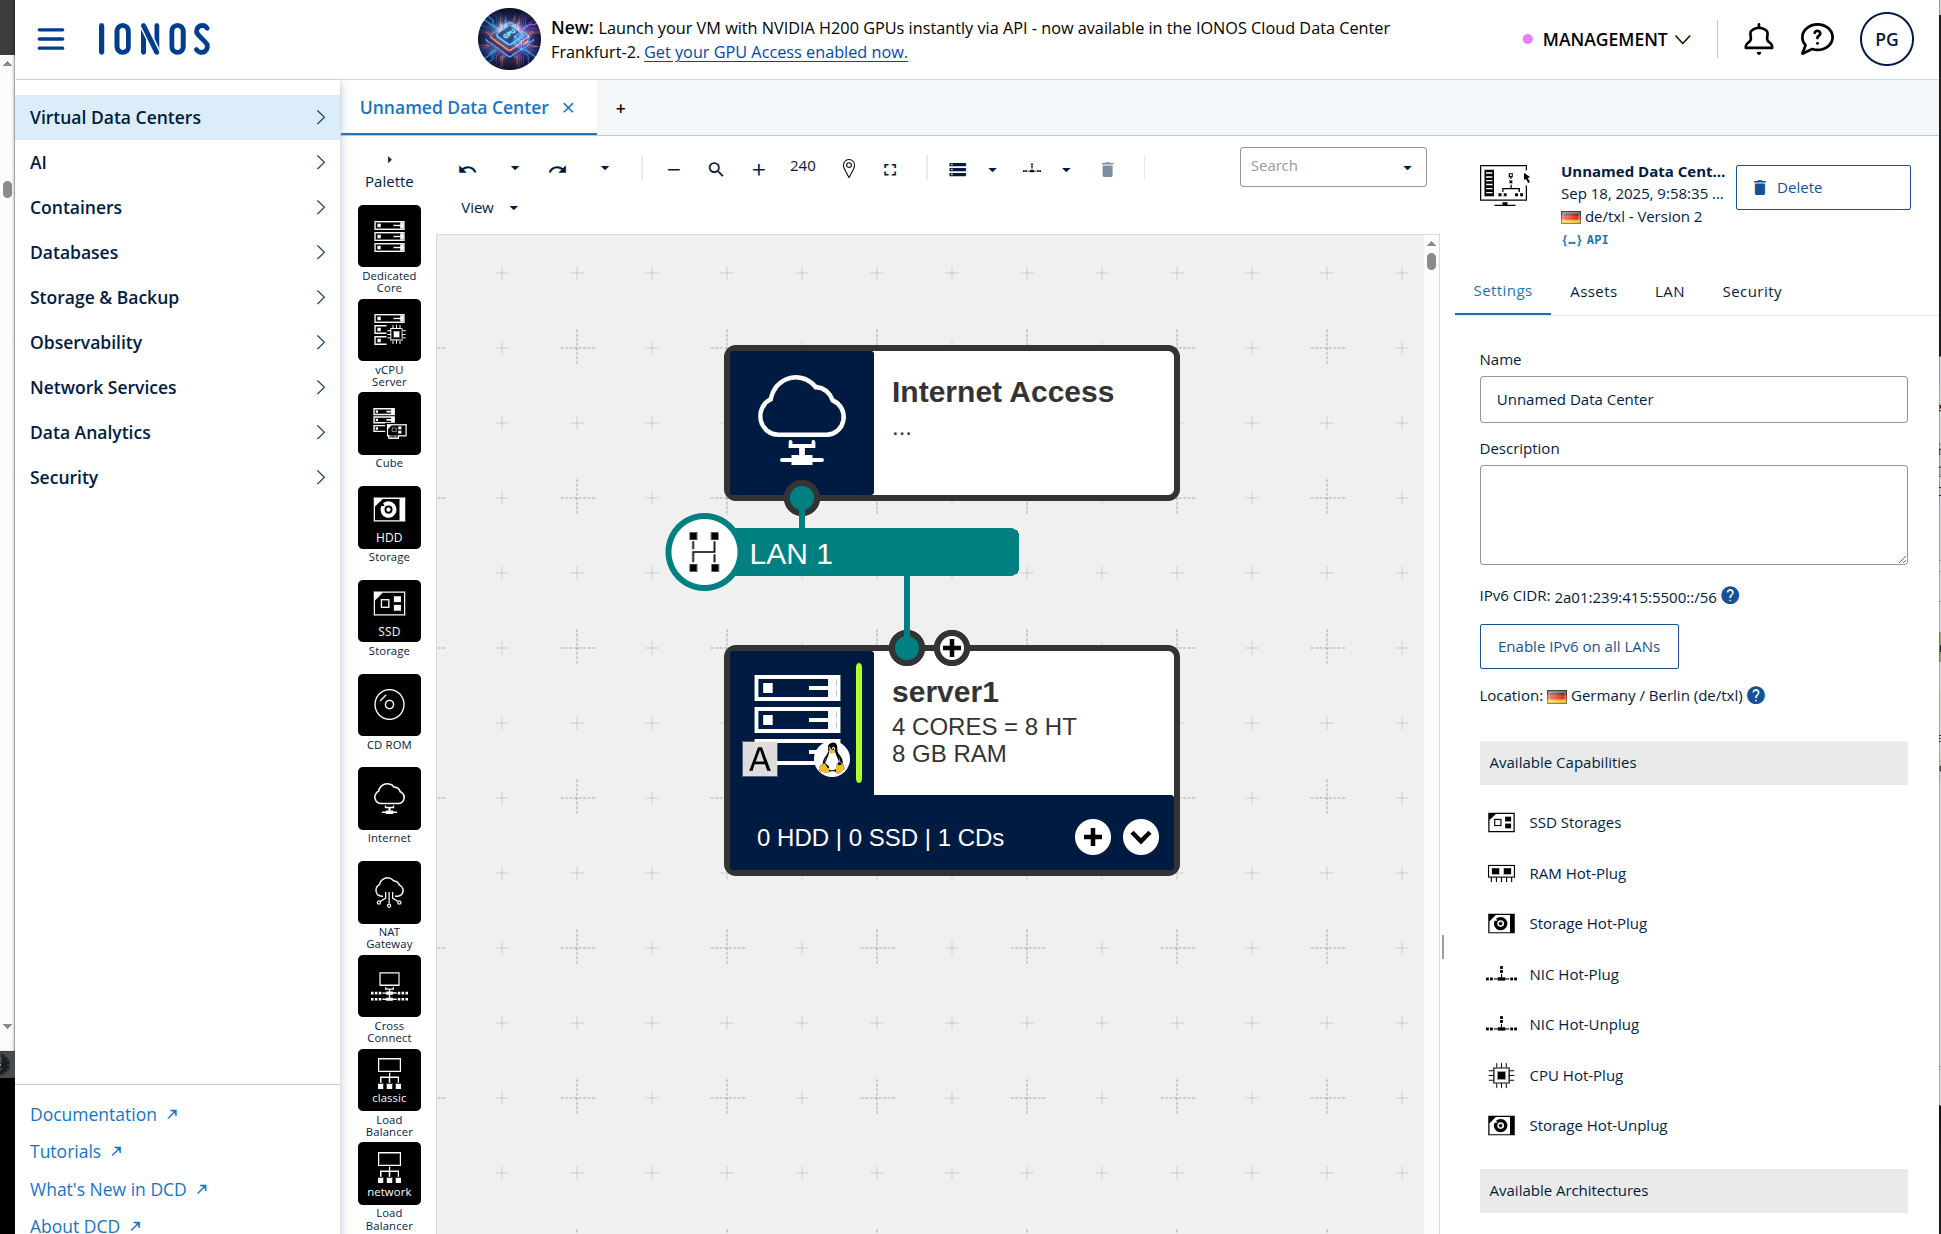
\includegraphics[width=13.5cm]{./imagenes/interfaz-DCD-2.png}
    \caption{Interfaz en Centro de Datos del DCD IONOS Cloud}
    \label{fig:dcd-arquitectura}
\end{figure}

\subsubsection{Herramientas del DCD}

El DCD tiene muchas herramientas y es importante conocerlas para este proyecto, porque para controlar la facturación hay que saber los tipos de elementos que forman el DCD.

\begin{enumerate}
    \item \textbf{Diseñador Gráfico: } Interfaz principal en la que se pueden añadir los recursos principales que se desglosan en el \hyperref[anexo:Lista-de-SKUs]{Anexo 1}.

    \item \textbf{Inteligencia Artificial: } Tiene una herramienta de apoyo de inteligencia artificial de varios modelos; se mide su uso por medio de \textit{tokens}\footnote{Un \textit{token} es una cadena alfanumérica única y secreta generada por un servidor para autenticar y autorizar a un cliente (aplicación, usuario o dispositivo) al realizar solicitudes.}.

    \item \textbf{Contenedores:} es la categoría que agrupa las herramientas para la modernización de aplicaciones (cloud-native). Ofrece dos servicios esenciales y sinérgicos:
          \begin{itemize}
              \item \textbf{Container Registry}: el ``dónde'' guardas tus componentes de software empaquetados (imágenes).
              \item \textbf{Managed Kubernetes}: el ``cómo'' los pones en producción de forma automática, escalable y resistente.
          \end{itemize}

    \item \textbf{Bases de datos: } Conjunto de datos organizado de tal modo que permita obtener con rapidez diversos tipos de información. Hay tanto relacionales como no relacionales, para más información consultar el anexo 1.

    \item \textbf{ Almacenamiento y Copias de Seguridad:} En el \textit{DCD}, Storage y Backup son pilares complementarios de la estrategia de datos, siendo el Almacenamiento donde ``viven'' mis datos ahora mismo y las copias de seguridad la manera de recuperar dicha información. Ofrece cinco servicios:
          \begin{itemize}
              \item \textbf{ IONOS Object Storage: } Almacén masivo para archivos y objetos.
              \item \textbf{ Network File Storage: } Sistema de archivos compartido en red.
              \item \textbf{ Backup Unit Manager: } Herramienta de automatización y gestión de copias de seguridad.
              \item \textbf{ Images y Snapshots: } Captura del estado del sistema para revertir o clonar.
              \item \textbf{ FTP Image Upload: } Importación de plantillas personalizadas de sistemas.
          \end{itemize}
    \item \textbf{Servicios de red: } Define cómo se conectan y comunican todos los recursos, es una de las partes más importantes, desglosándose en varias partes:
          \begin{itemize}
              \item \textbf{Administración de direcciones IP: } gestión centralizada de direcciones IP.
              \item \textbf{Puerta de Enlace VPN: }  Servicio que crea un túnel cifrado y seguro entre tu infraestructura en IONOS Cloud y otro sitio.
              \item \textbf{Red de Distribución de Contenidos: } Una red global de servidores que almacenan en caché copias del contenido est\'atico (im\'agenes, CSS{\textgreater}, JS{\textgreater}, videos) cerca de los usuarios finales.
              \item \textbf{Cloud DNS: } El servicio de resolución de nombres de dominio gestionado por IONOS. Traduce nombres de dominio (www.tuempresa.com) a direcciones IP (185.100.100.10).
          \end{itemize}
    \item \textbf{Seguridad: } Marco de trabajo integrado que aplica múltiples capas de protección:
          \begin{itemize}
              \item \textbf{Manager de llaves SSH:} protege el ``quién''; autenticación fuerte para administradores y automatización.
              \item \textbf{Grupos de Seguridad de Red:} protege el ``qué y dónde''; control estricto del flujo de tráfico entre los recursos.
              \item \textbf{ Gestor de certificados: } protege el ``cómo''; confianza y privacidad para las comunicaciones con los usuarios finales.
          \end{itemize}
\end{enumerate}


% ===== SECCIÓN 1.3: ¿QUÉ ES UNA API CANARY? =====
\section{¿Qué es una API REST y una API Canary?}\label{sec:api-canary}

\subsection{¿Qué es una API REST?}
Una API REST es un intermediario estandarizado que permite que diferentes aplicaciones se comuniquen entre sí mediante el protocolo HTTP.
En el contexto de este proyecto, la API REST desarrollada permite ejecutar y gestionar los tests de validación de facturación, comunicándose
con los servicios de IONOS Cloud para obtener datos de consumo y compararlos con los cargos facturados. Este formato fue requerido por la empresa debido a
su escalabilidad, simplicidad y naturaleza sin estado (cada petición es independiente y autocontenida).
\subsection{Principios REST}
\begin{itemize}
    \item \textbf{Arquitectura Cliente-Servidor: } Clara separación entre el cliente (solicita) y el servidor (responde). En este proyecto, la API de validación actúa como servidor que recibe peticiones y se comunica con los servicios de facturación de IONOS Cloud.
    \item \textbf{Sin Estado: } Cada petición contiene toda la información necesaria. En el proyecto, cada llamada de validación incluye el token de autenticación y los parámetros del test a ejecutar.
    \item \textbf{Cacheable: } Las respuestas pueden almacenarse temporalmente. Esto permite optimizar las consultas repetidas a datos de facturación que no cambian frecuentemente.
    \item \textbf{Interfaz Uniforme: } Todo es un recurso con URI única. La API expone endpoints claros como \texttt{/validation}, \texttt{/products} o \texttt{/utilization}.
    \item \textbf{Sistema en Capas: } El cliente no sabe si está conectado al servidor final o a un intermediario. El sistema puede escalarse añadiendo proxies o balanceadores sin modificar los clientes.

\end{itemize}

\subsection{Concepto y Origen de API Canary}

El término \textbf{``Canary''} proviene de la práctica minera de usar canarios para detectar gases peligrosos. En desarrollo de software, una \textbf{API Canary} se refiere a:

\begin{quote}
    Una implementación de API que se despliega gradualmente a un subconjunto de usuarios o sistemas para detectar posibles problemas antes de que el usuario final lo detecte. El método de funcionamiento es una ejecución periódica con una alarma si falla, la frecuencia de dicha ejecución será dependiente de lo crítico que sea el módulo que controla.
\end{quote}

\subsection{Características Principales}

\begin{table}[h!]
    \centering
    \begin{tabular}{|p{0.3\textwidth}|p{0.6\textwidth}|}
        \hline
        \textbf{Característica}                                                                                                                                                           & \textbf{Descripción}                                       \\
        \hline
        \hline
        \textbf{Despliegue Gradual}                                                                                                                                                       & Se implementa primero a un pequeño porcentaje del tráfico. \\
        \hline
        \textbf{Monitorización Intensiva}                                                                                                                                                 & Se supervisa exhaustivamente en busca de errores.          \\
        \hline
        \textbf{Rollback Automático}                                                                                                                                                      & Si se detectan problemas, se revierte automáticamente.     \\
        \hline
        \textbf{A/B \textit{Testing}\footnote{Es el proceso de evaluar, verificar y validar software u otros sistemas para asegurar que funcionan según lo esperado, detectando errores}} & Permite comparar versiones nuevas vs. antiguas.            \\
        \hline
    \end{tabular}
    \caption{Características de una API Canary}
    \label{tab:api-canary-caracteristicas}
\end{table}

\subsection{Ventajas en Sistemas de Facturación}

La implementación de APIs Canary en sistemas de facturación ofrece:

\begin{itemize}
    \item \textbf{Detección temprana}: Problemas se identifican rápidamente, el tiempo que tarde en detectarse será dependiente de la frecuencia de su ejecución.
    \item \textbf{Reducción de riesgos}: Errores de facturación afectan solo a un subconjunto de clientes. Ya que al detectarse de forma temprana y le afecta a menos clientes.
    \item \textbf{Validación en producción}: Pruebas con datos reales sin comprometer todo el sistema. Ya que se crea un cliente real completo para usar en la API.
    \item \textbf{Mejora continua}: Permite iteraciones rápidas y seguras. Ya que es muy fácil de separar en módulos.
\end{itemize}



\subsection{Flujo de Trabajo Canary}

\begin{figure}[h!]
    \centering
    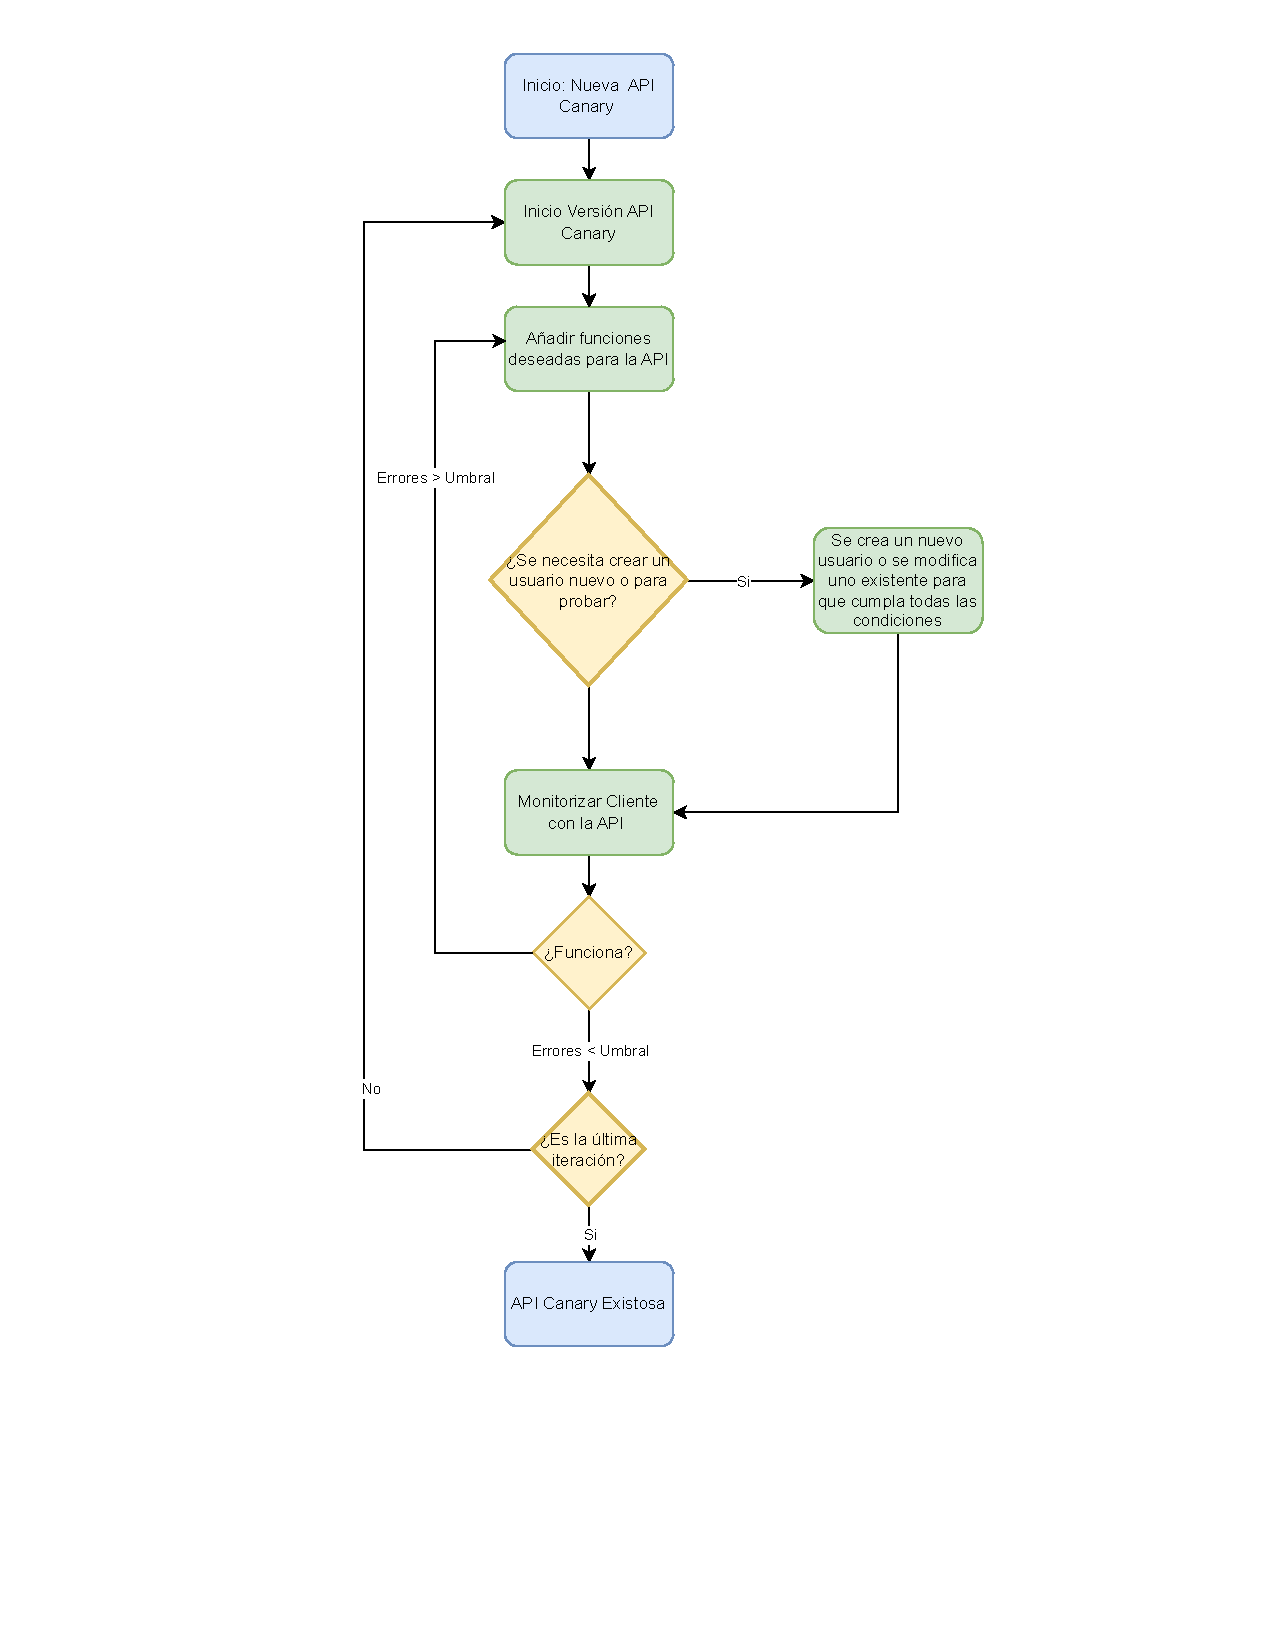
\includegraphics[width=0.9\textwidth]{archivos/flujo_API_Canary.drawio.pdf}
    \caption{Diagrama de flujo del proceso de despliegue Canary para APIs}
    \label{fig:canary-flow}
\end{figure}

\textbf{Descripción del flujo:}
\begin{enumerate}
    \item \textbf{Inicio: Nueva API Canary } - Desarrollo de una nueva  API de validación.

    \item \textbf{Inicio: Nueva Versión API Canary} - Desarrollo de una nueva versión de la API de validación. En la que se inicia la nueva iteración.

    \item \textbf{Inicio: Añadir funciones deseadas} - Se implementan las nuevas funciones deseadas.

    \item \textbf{Comprobación de completitud del usuario de muestra} - Se comprueba que el usuario que se usa para comprobar el correcto funcionamiento de la API tiene todos los recursos necesarios que debe comprobar. En el caso contrario, se modifica para que permita comprobar todas las funciones a comprobar, en su defecto se creará un nuevo perfil para ello.

    \item \textbf{Monitorizar Métricas} - Análisis continuo de errores, latencia y otras métricas clave.

    \item \textbf{Decisión basada en umbrales:}
          \begin{itemize}
              \item \textbf{Si errores < Umbral} → Se pasa a la siguiente fase de la API.
              \item \textbf{Si errores > Umbral} → Rollback automático a versión estable y se revisan las actualizaciones para volver a modificar y lograr hacer funcionales los cambios.
          \end{itemize}

    \item \textbf{API Canary Exitosa} - Tras terminar todas las fases, se integra y entra la fase de automatizarla para que se ejecute periódicamente.
\end{enumerate}

% ===== SECCIÓN 1.4: TECNOLOGIAS Y HERRAMIENTAS =====

\section{Tecnologías y Herramientas Utilizadas}

\noindent Para el desarrollo del sistema de validación de facturación cloud, se ha construido una arquitectura tecnológica robusta que combina herramientas modernas de desarrollo, infraestructura contenerizada y patrones de diseño específicos para el dominio de facturación.

\subsubsection{Stack Tecnológico Principal}

\begin{table}[h!]
    \centering
    \begin{tabular}{|p{0.25\textwidth}|p{0.7\textwidth}|}
        \hline
        \textbf{Categoría}                         & \textbf{Tecnologías}                    \\
        \hline
        \hline
        \textbf{Runtime}                           & Node.js 18+ (LTS)                       \\
        \hline
        \textbf{Lenguaje}                          & JavaScript ES6+ con módulos             \\
        \hline
        \textbf{Framework Web}                     & Express.js con middleware personalizado \\
        \hline
        \textbf{Gestión de Paquetes}               & Yarn 3+ con workspace                   \\
        \hline
        \textbf{Testing}                           & Postman                                 \\
        \hline
        \textbf{Creación de usuarios de muestreo } & DCD de IONOS                            \\
        \hline
        \textbf{Base de Datos Configuración}       & CouchDB para configuración distribuida  \\
        \hline
        \textbf{Control de Versiones}              & GitLab para paquetes internos           \\
        \hline
        \textbf{Editor de Código}                  & Visual Studio Code                      \\
        \hline
        \textbf{Documentación}                     & LaTeX en OverLeaf                       \\
        \hline
        \textbf{Creación de diagramas}             & Draw.io                                 \\
        \hline
        \textbf{Conexión con equipo }              & VPN a red Alemana                       \\
    \end{tabular}
    \caption{Stack tecnológico del proyecto}
    \label{tab:stack-tecnologico}
\end{table}

\subsubsection{Dependencias Clave del Proyecto}

\textbf{Dependencias Internas:}
\begin{itemize}
    \item \texttt{@internal/core} - Framework base con utilidades de inicialización y configuración
    \item \texttt{@internal/dev} - Suite de herramientas para desarrollo y debugging
\end{itemize}

\textbf{Dependencias Externas Críticas:}
\begin{itemize}
    \item \texttt{helmet} - Middleware de seguridad para cabeceras HTTP
    \item \texttt{express} - Framework web minimalista para Node.js
    \item \texttt{couchdb-nano} - Cliente para integración con CouchDB
\end{itemize}

\subsubsection{Arquitectura Modular Implementada}

La arquitectura del sistema se organiza en tres capas principales:

\begin{enumerate}
    \item \textbf{Capa de Infraestructura:}
          \begin{itemize}
              \item CouchDB para gestión de configuración centralizada
          \end{itemize}

    \item \textbf{Capa de Servicios:}
          \begin{itemize}
              \item \texttt{data-api}: Servicio de acceso y transformación de datos
              \item \texttt{invoice-validation}: Motor de validación de facturación
              \item \texttt{utilization}: Procesamiento de métricas de uso
          \end{itemize}

    \item \textbf{Capa de Helpers y Utilidades:}
          \begin{itemize}
              \item Módulo \texttt{schema}: Validación y transformación de datos
              \item Módulo \texttt{actions}: Operaciones comunes del negocio
              \item Módulo \texttt{invoice}: Lógica específica de facturación
          \end{itemize}
\end{enumerate}

\subsubsection{Flujo de Desarrollo y Calidad}

\begin{itemize}
    \item \textbf{Desarrollo Local:} Nodemon para hot-reload durante el desarrollo
    \item \textbf{Calidad de Código:} ESLint con configuración personalizada
    \item \textbf{Control de Cambios:} Hooks pre-commit para validaciones automáticas
    \item \textbf{Integración:} Pipelines CI/CD en GitLab para despliegue continuo
\end{itemize}


\newpage

% ============================================
% ===== CAPÍTULO 2: ANÁLISIS =====
% ============================================
\chapter{Análisis}\label{chap:analisis}
En este capítulo se define el proyecto, creando los requisitos para la identificación de los requisitos funcionales y no funcionales. Después de obtener dichos requisitos, se limitará el proyecto mediante un estudio de viabilidad debido a la limitación de recursos, en concreto el tiempo. En caso de ser viable, se realizará y en caso negativo se limitará a una parte de dicho proyecto que proporcione un conjunto modular funcional.

\section{Definición y alcance del proyecto}
\subsubsection{Definición del Proyecto}

El proyecto \textbf{API Canary de Validación de Facturación Cloud} consiste en el desarrollo e implementación de un sistema de validación cruzada automatizada para los procesos de facturación de IONOS Cloud. Esta solución implementa una arquitectura de despliegue gradual (Canary) que permite la detección temprana de inconsistencias mediante la comparación de resultados entre sistemas independientes.

La API actúa como un \textit{sistema de alerta temprana} que ejecuta validaciones periódicas sobre los datos de facturación generados por el Data Center Designer (DCD), comparándolos con los sistemas legacy de facturación para garantizar coherencia y precisión en los cargos a los clientes.

\subsubsection{Alcance Técnico}

\begin{itemize}
    \item \textbf{Desarrollo de API REST:} Implementación de \textit{endpoints}\footnote{Es la URL específica y única (https://api.ejemplo.com/usuarios) que permite a una aplicación cliente interactuar con un servidor para acceder, modificar o enviar recursos específicos.}  para ejecución, programación y monitoreo de validaciones.
    
    \item \textbf{Sistema de Despliegue Canary:} Mecanismos para implementaciones graduales con capacidad de rollback automático. Basado en GitLab.
    
    \item \textbf{Validación Cruzada:} Comparación automática entre:
    \begin{itemize}
        \item Datos del DCD (Data Center Designer).
        \item Cálculos teóricos reales del coste.
    \end{itemize}
    
    \item \textbf{Monitoreo y Alertas:} Sistema de notificaciones en tiempo real ante discrepancias detectadas.
\end{itemize}

\subsubsection{Alcance Funcional}

El sistema cubre las siguientes funcionalidades principales:

\begin{enumerate}
    \item \textbf{Validación Automatizada:}
    \begin{itemize}
        \item Ejecución programada de validaciones (diaria, semanal, mensual).
        \item Verificación de consistencia en cálculos de facturación.
        \item Detección de discrepancias en precios y tarifas.
    \end{itemize}
    
    \item \textbf{Gestión de Configuración:}
    \begin{itemize}
        \item Administración de reglas de validación.
        \item Configuración de umbrales de tolerancia.
        \item Gestión de frecuencias de ejecución.
    \end{itemize}
    
    \item \textbf{Reporting y Dashboard:}
    \begin{itemize}
        \item Generación de reportes de validación.
        \item Dashboard de métricas y KPIs.
        \item Histórico de discrepancias detectadas.
    \end{itemize}
    
    \item \textbf{Integraciones:}
    \begin{itemize}
        \item Conexión con sistemas DCD de IONOS.
        \item Comunicación con sistemas de alertas (Slack, Email, Teams).
    \end{itemize}
\end{enumerate}

\subsubsection{Límites y Exclusiones}

\begin{itemize}
    \item \textbf{No incluye:} Modificación de sistemas legacy de facturación.
    \item \textbf{No incluye:} Desarrollo de interfaz gráfica de usuario (GUI) completa.
    \item \textbf{No incluye:} Gestión de reclamaciones de clientes.
    \item \textbf{Se limita a:} Entornos de desarrollo, testing y producción de IONOS Cloud.
    \item \textbf{Se limita a:} Validación de facturación del DCD de IONOS cloud (no otros productos).
\end{itemize}

\newpage

\subsubsection{Objetivos de Calidad}

\begin{table}[htbp]
    \centering
    \begin{tabular}{|p{0.35\textwidth}|p{0.25\textwidth}|p{0.3\textwidth}|}
    \hline
    \textbf{Métrica} & \textbf{Objetivo} & \textbf{Justificación} \\
    \hline
    \hline
    Tiempo de detección de errores & < 24 horas & Minimizar impacto en clientes \\
    \hline
    Precisión en validación de elementos estáticos & 99.9\% & Garantizar fiabilidad de facturación \\
    \hline
    Cobertura de tests & > 95\% & Calidad del código y funcionalidad \\
    \hline
    \end{tabular}
    \caption{Métricas de calidad del proyecto}
    \label{tab:metricas-calidad}
\end{table}

\subsubsection{Entregables del Proyecto}

\begin{itemize}
    \item \textbf{Código En este capítulo se define el proyecto, creando los requisitos para la identificación de los requisitos funcionales y no funcionales. Después de obtener dichos requisitos se limitará el proyecto teniendo, por medio de un estudio de viabilidad debido a la limitación de recursos, en concreto el tiempo. En caso de ser viable se realizara y en caso negativo se limitara a una parte de dicho proyecto que proporcione un cpnjunto modular funcional. fuente:} Repositorio Git con toda la implementación.
    \item \textbf{Memoria de implementación:} Documentación del proceso y de lecciones aprendidas.
\end{itemize}

\section{Requisitos}
A partir del punto anterior se desarrollarán los siguientes requisitos:
\begin{table}[htbp]
    \centering
    \begin{tabular}{|p{0.1\textwidth}|p{0.7\textwidth}|}
    \hline
    \multicolumn{2}{|c|}{\textbf{Requisitos no Funcionales}} \\
    \hline
    \hline
    Código &  Descripción \\
    \hline
    RNF01 & Fiabilidad, tener garantías del correcto funcionamiento\\
    \hline
    RNF02 & Mantenibilidad, teniendo que ser fácil la actualización y fácil adición de nuevos tipos de recursos\\
    \hline
    RNF03 & Seguridad, Credenciales seguras para las APIs y accesos restringidos al contrato de pruebas. \\
    \hline
    RNF04 & Costos, minimización de los costos de recursos de prueba \\
    \hline   
    \end{tabular}
    \caption{Requisitos no funcionales}
    \label{tab:requisitos-no-funcionales}
\end{table}

\begin{table}[htbp]
    \centering
    \begin{tabular}{|p{0.1\textwidth}|p{0.55\textwidth}|}
    \hline
    \multicolumn{2}{|c|}{\textbf{Requisitos Funcionales}} \\
    \hline
    \hline
    Código &  Descripción \\
    \hline
    \multicolumn{2}{|c|}{\textbf{RF01 - Gestión del Contrato de Pruebas}} \\
    \hline
    RF01.01 & El sistema debe tener un usuario exclusivo para las pruebas de facturación. \\
    \hline
    RF01.02 & El contrato del usuario debe tener todos los recursos facturables del producto. \\
    \hline
    RF01.03 & Exclusión manual de productos con costos de licencia elevados cuando sea posible \\
    \hline
    \multicolumn{2}{|c|}{\textbf{RF02 - Recursos de Consumo Constante (Continuables)}} \\
    \hline
    RF02.01 & Provisión automática de recursos que mantienen consumo constante \\
    \hline
    RF02.01.01 & Provisión automática de Maquinas Virtuales (VMs) \\
    \hline
    RF02.01.02 & Provisión automática de Almacenamiento (S3 buckets, discos) \\
    \hline
    RF02.02& Configuración única sin modificaciones posteriores \\
    \hline
    RF02.03& Consumo mensual predecible y estable, no introducir cambios bruscos\\
    \hline
    \multicolumn{2}{|c|}{\textbf{RF03 - Generación de Consumo Variable (No Continuables)}} \\
    \hline
    RF03.01 & Servicio Canary API para generar consumo artificial \\
    \hline
    RF03.02 & Generación de cantidades similares mensualmente \\
    \hline
    RF03.03 & Tolerancia configurable para variaciones esperadas \\
    \hline
    RF03.04 & Programación de jobs cron para generación periódica \\
    \hline
    \multicolumn{2}{|c|}{\textbf{RF04 - Verificación de Facturación}} \\
    \hline
    RF04.01 & Recolección diaria de datos de consumo \\
    \hline
    RF04.02 & Comparación con cálculos dinámicos generados automáticamente \\
    \hline
    RF04.03 & Márgenes de tolerancia configurables por \textit{SKU}\footnote{Código alfanumérico único que cada empresa crea para identificar y gestionar una variante específica de un producto.}\\
    \hline
    \multicolumn{2}{|c|}{\textbf{RF05 - Sistema de Alertas y Reportes}} \\
    \hline
    RF05.01 & Notificaciones automáticas en desviaciones significativas \\
    \hline
    RF05.04 & Histórico de verificaciones y desviaciones \\
    \hline
    
    \end{tabular}
    \caption{Requisitos funcionales}
    \label{tab:requisitos-funcionales}
\end{table}

\newpage

\section{Estudio de viabilidad}
\subsection{Requisitos mínimos}
\begin{itemize}
    \item \textbf{Usuario con contrato: } Se necesita un contrato con capacidad de recursos mayor a un contrato estándar del DCD de IONOS, ya que se necesitan recursos extra para poder lograr usar todos los elementos a estudiar. En este caso no hay problema, ya que al ser el DCD de IONOS un servicio nuestro, se puede solicitar dicho contrato ampliado.
    \item \textbf{Acceso a APIs internas: }Se necesita acceso a estas APIs como por ejemplo \textit{IONOS Cloud Billing API (3.9.0)}, siendo esta imprescindible, ya que es de donde se sacarán los datos a comparar y usar. Una vez conseguido el contrato se puede adquirir de forma natural. 
    \item \textbf{Aceso a Base de datos de configuración: }Se necesita acceso a la base de datos de \textit{Apache CouchDB} porque es la Base de Datos usada para las configuraciones y tiene acceso restringido. El acceso a esta página web es más complejo, pero solicitándolo con tiempo es posible. 
\end{itemize}
\subsection{Viabilidad de constancia de recursos a analizar}
    Hay dos tipos, los \textit{items} continuables y los no continuables, siendo los continuables, los que son recursos que todos los meses son iguales, como por ejemplo una máquina virtual o una \textit{IP}. Por otro lado están los recursos no continuables, siendo estos los que no tienen por qué ser todos los meses iguales, como puede ser por ejemplo el uso de \textit{tokens} de uso de una Inteligencia Artificial. 
    \begin{itemize}
        \item \textbf{items continuables :} La constancia de estos recursos es sencilla, el único problema posible es añadir todos los recursos que se quieren comprobar, ya que no hay una clara vinculación entre los items y luego su representación gráfica en la interfaz del DCD. 
        \item \textbf{items no continuables :} La continuidad de estos items es más compleja, debido a que no hay forma de que todos los meses sea exactamente igual y que uso debe ser de manera manual o automatizada cada mes, por lo que se debe hacer un estudio más desarrollado.
    \end{itemize}
    
    
    
    





\newpage

% ============================================
% ===== CAPÍTULO 3: PLANIFICACIÓN =====
% ============================================
\chapter{Planificación}\label{chap:planificacion}
Una vez definidos los requisitos y la metodología a seguir, el siguiente paso es planificar de forma concreta el proyecto. En esta fase se crearán los distintos módulos del proyecto (EDT), se establecerán las fechas límite para los entregables y se estimará el tiempo necesario para cada apartado. Además, se incluirá un cronograma de hitos y un diagrama del flujo de trabajo. Posteriormente, se diseñará un plan de gestión de riesgos basándose en la metodología aprendida durante la carrera. El capítulo concluye con la descripción de las tecnologías utilizadas.

\section{Descomposición del Proyecto (EDT)}
\begin{figure}[h!]
    \centering
    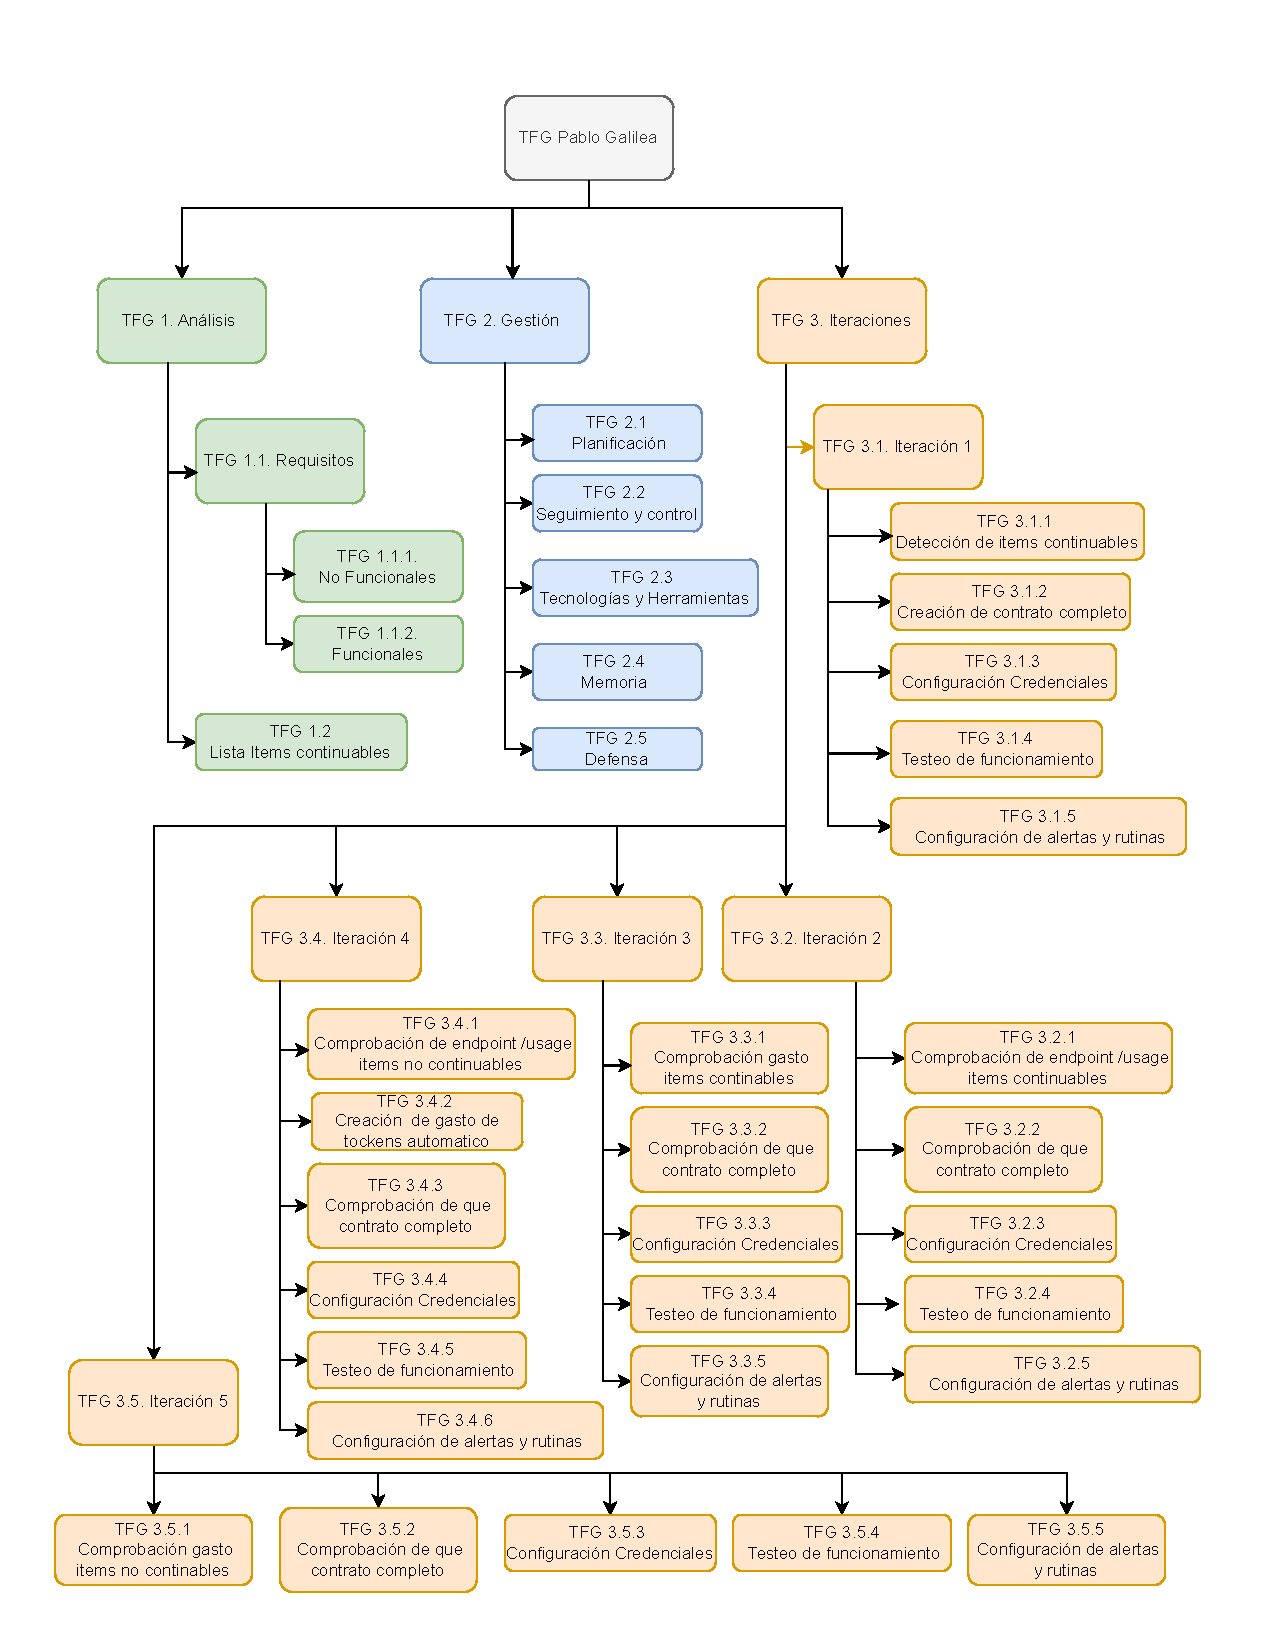
\includegraphics[width=0.6\textwidth]{archivos/EDT.pdf}
    \caption{EDT}
    \label{fig:edt}
\end{figure}
\subsection{Explicación del EDT}
En este apartado se describirán los diferentes módulos del EDT relacionandolos con los requisitos.
\begin{enumerate}
    % Configurar todos los niveles primero
    \renewcommand{\theenumii}{\theenumi.\arabic{enumii}}
    \renewcommand{\theenumiii}{\theenumii.\arabic{enumiii}}
    \renewcommand{\labelenumii}{\theenumii}
    \renewcommand{\labelenumiii}{\theenumiii}

    \item \textbf{Análisis}
          \begin{enumerate}
              \item \textbf{Análisis de Requisitos:} Identificación, documentación y validación de las necesidades del proyecto para definir las funcionalidades (funcionales) y restricciones (no funcionales) de un sistema.
                    \setcounter{enumiii}{0} % Reiniciar contador del tercer nivel
                    \begin{enumerate}
                        \item \textbf{No Funcionales:} Lista de aquellos requisitos que, aunque no añaden funcionalidad al proyecto, son importantes a tener en cuenta para lograr su ejecución.
                        \item \textbf{Funcionales:} Lista de aquellos requisitos necesarios para lograr que el proyecto cumpla con todas las características necesarias para que sea funcional.
                    \end{enumerate}
              \item \textbf{Lista de items continuables:} Lista con todos los SKUs de los recursos activos del DCD, omitiendo los obsoletos. Esta lista es necesaria para cumplir el requisito RF01.02 y permite identificar los elementos de mayor coste, información requerida para el requisito RF01.03 y RNF04.
          \end{enumerate}

    \item \textbf{Gestión}
          \setcounter{enumii}{0} % Reiniciar contador del segundo nivel
          \begin{enumerate}
              \item \textbf{Planificación: } Proceso de definir objetivos, tareas, recursos, costos y cronogramas para guiar la ejecución y asegurar el éxito, en el que se decide y especifica el cumplimiento de los requisitos RNF05 a RNF09.
              \item  \textbf{Seguimiento y Control: }Tras la implementación y la finalización del proyecto se hace un seguimiento de su correcto funcionamiento. Fundamental para lograr el requisito RNF01 y RNFO2.
              \item \textbf{Tecnologías y Herramientas: } Son las metodologías y enfoques que se han usado para la elaboración del proyecto y desarrollan los requisitos RNF05 a RNF09
              \item \textbf{Memoria:} El proceso de documentación del proyecto para poder analizarlo.
              \item \textbf{Defensa:} Argumentos y explicación sobre el proyecto para poder exponerlo a un tribunal ante posibles dudas.
          \end{enumerate}

    \item \textbf{Iteraciones}
          \setcounter{enumii}{0} % Reiniciar contador del segundo nivel
          \begin{enumerate}
              \item \textbf{Iteración 1:} Siendo esta la primera iteración, es en la que se crea la base en la que se basarán el resto de iteraciones, por lo que se deben tomar sus decisiones teniendo en cuenta que podrían afectar al resto del proceso. En esta primera iteración se detectarán los elementos que forman un contrato.
                    \setcounter{enumiii}{0} % Reiniciar contador del tercer nivel si es necesario
                    \begin{enumerate}
                        \item \textbf{Detección de items continuables:} La funcionalidad añadida en esta primera iteración se basa en lograr detectar qué SKUs forman parte de la lista creada. Como el contrato será creado por nosotros, se añadirán todos los SKUs, así que todos deberán estar; todo el que falte será un falso positivo.
                        \item \textbf{Creación de contrato completo:} De manera manual se crea un contrato con todos los SKUs de la lista. Cumpliendo asi el requisito RF01.01, RF02.01,RF02.01.01,RF02.01.02 y RF02.03.
                        \item \textbf{Configuración de Credenciales:} Esto se hace en todas las iteraciones, por lo que no se explicará en el resto, solo en esta. Se basa en la configuración concreta de CouchDB para el correcto funcionamiento. Cumpliendo así el requisito RF02.02.
                        \item \textbf{Testeo de funcionamiento: } Al igual que el anterior, este paso se hace en todas las iteraciones, por lo que solo se explicará en esta. En este apartado se crean las comprobaciones del correcto funcionamiento de esta y de las anteriores iteraciones.
                        \item \textbf{Configuración de alertas y rutinas: } Este apartado tiene la misma peculiaridad que los otros dos anteriores, por lo que se explicará solo en esta ocasión y se basa en crear las alertas que se enviarán en caso de fallo dependiendo de la información que ya se disponga, en este caso los SKUs que faltan y también crear el disparador para que se ejecute en cierto momento.

                    \end{enumerate}


              \item \textbf{Iteración 2:} En esta iteración ya se implementa el medir el uso de los SKUs continuables detectados en la iteración anterior y compararla con la esperada.
                    \setcounter{enumiii}{0} % Reiniciar contador del tercer nivel si es necesario
                    \begin{enumerate}
                        \item \textbf{Detección de endpoint /usage items continuables: } Para comprobar el uso de los elementos del DCD por medio de su API se puede comprobar con /usage.
                        \item \textbf{Comprobación de que contrato completo:} Se comprueba que no haya que añadir nada nuevo al contrato, en caso de ser necesario se añade y como será igual en el resto de iteraciones tampoco se añadirá.
                    \end{enumerate}


              \item \textbf{Iteración 3:} En esta iteración sabiendo el uso de los diferentes elementos se calcula su gasto económico teórico y se comprueba con el real.
                    \setcounter{enumiii}{0} % Reiniciar contador del tercer nivel si es necesario
                    \begin{enumerate}
                        \item \textbf{Comprobación gasto items continuables: } Sabiendo el gasto se calcula el precio de cada uno y se compara con el proporcionado por la API.
                    \end{enumerate}


              \item \textbf{Iteración 4:} En esta iteración se pasa a los items no continuables, por lo que se estudia cómo hacer un gasto relativamente constante de estos.
                    \setcounter{enumiii}{0} % Reiniciar contador del tercer nivel si es necesario
                    \begin{enumerate}
                        \item \textbf{Comprobación de endpoint /usage items no continuables: } Se comprueba el gasto de items no continuables por medio de su SKU.
                        \item \textbf{Creación de gasto de tokens automático:} Se estudia cómo lograr un gasto lo más constante posible de tokens.
                    \end{enumerate}


              \item \textbf{Iteración 5:} Teniendo ya el gasto, se calcula su precio y se comprueba con el gasto proporcionado por la API.
                    \setcounter{enumiii}{0} % Reiniciar contador del tercer nivel si es necesario
                    \begin{enumerate}
                        \item \textbf{Comprobación gasto items no continuables:} Se comprueba el gasto económico de items no continuables por medio de su SKU comparándolo con el obtenido en la API.
                    \end{enumerate}
          \end{enumerate}
\end{enumerate}
\newpage

\section{Estimación de tiempos}




\begin{table}[h!]
    \centering
    \small
    \begin{tabular}{|c|c|c|c|}
        \hline
        \multicolumn{4}{|c|}{Plan de dedicación de tiempo}                                                                       \\
        \hline
        Bloque                               & Nodo                                             & Tiempo & Total                 \\
        \hline
        \multirow{3}{*}{Análisis}            & Lista requisitos funcionales                     & 5h     & \multirow{3}{*}{15h}  \\
        \cline{2-3}
                                             & Análisis de requisitos Funcionales               & 5h     &                       \\
        \cline{2-3}
                                             & Análisis de requisitos no Funcionales            & 5h     &                       \\
        \hline
        \multirow{5}{*}{Gestión}             & Planificación                                    & 35h    & \multirow{5}{*}{141h} \\
        \cline{2-3}
        Cronograma de tareas                 & Seguimiento y control                            & 10h    &                       \\
        \cline{2-3}
                                             & Tecnologías y Herramientas                       & 6h     &                       \\
        \cline{2-3}
                                             & Memoria                                          & 75h    &                       \\
        \cline{2-3}
                                             & Defensa                                          & 15h    &                       \\
        \hline
        \multirow{5}{*}{Iteración 1}         & Detección de items continuables                  & 16h    & \multirow{5}{*}{42h}  \\
        \cline{2-3}
                                             & Creación de contrato completo                    & 12h    &                       \\
        \cline{2-3}
                                             & Configuración de credenciales                    & 6h     &                       \\
        \cline{2-3}
                                             & Testeo de funcionamiento                         & 4h     &                       \\
        \cline{2-3}
                                             & Configuración de alertas y rutinas               & 4h     &                       \\
        \hline
        \multirow{5}{*}{Iteración 2}         & Comprobación de /usage items continuables        & 16h    & \multirow{5}{*}{21h}  \\
        \cline{2-3}
                                             & Comprobación de que contrato completo            & 1h     &                       \\
        \cline{2-3}
                                             & Configuración de credenciales, alertas y rutinas & 2h     &                       \\
        \cline{2-3}
                                             & Testeo de funcionamiento                         & 2h     &                       \\
        \hline
        \multirow{5}{*}{Iteración 3}         & Comprobación gasto items continuables            & 16h    & \multirow{5}{*}{23h}  \\
        \cline{2-3}
                                             & Comprobación de que contrato completo            & 1h     &                       \\
        \cline{2-3}
                                             & Configuración de credenciales ,alertas y rutinas & 2h     &                       \\
        \cline{2-3}
                                             & Testeo de funcionamiento                         & 4h     &                       \\
        \hline
        \multirow{6}{*}{Iteración 4}         & Comprobación de /usage items no continuables     & 12h    & \multirow{6}{*}{37h}  \\
        \cline{2-3}
                                             & Creación de gasto de tokens automático           & 16h    &                       \\
        \cline{2-3}
                                             & Comprobación de que contrato completo            & 1h     &                       \\
        \cline{2-3}
                                             & Configuración de credenciales, alertas y rutinas & 4h     &                       \\
        \cline{2-3}
                                             & Testeo de funcionamiento                         & 4h     &                       \\
        \hline
        \multirow{5}{*}{Iteración 5}         & Comprobación gasto items no continuables         & 10h    & \multirow{5}{*}{21h}  \\
        \cline{2-3}
                                             & Comprobación de que contrato completo            & 1h     &                       \\
        \cline{2-3}
                                             & Configuración de credenciales, alertas y rutinas & 4h     &                       \\
        \cline{2-3}
                                             & Testeo de funcionamiento                         & 6h     &                       \\
        \hline
        \multicolumn{2}{|c|}{Total de Horas} & \multicolumn{2}{|c|}{300 h}                                                       \\
        \hline
    \end{tabular}
    \caption{Plan de dedicación de tiempos}
\end{table}

\section{Cronograma e hitos}

% Definir colores
\definecolor{ganttblue}{RGB}{173,216,230}
\definecolor{ganttgreen}{RGB}{144,238,144}



\begin{table}[h!]
    \centering
    \footnotesize
    \setlength{\tabcolsep}{3pt}
    \begin{tabular}{|c|l|c|c|c|c|c|c|c|c|c|c|c|c|} % <- segunda columna: l
        \hline
        \multicolumn{14}{|c|}{\textbf{Cronograma de tareas}}                                                                                                                                                                                                                                                                                                                  \\
        \hline
        \multicolumn{2}{|c|}{\multirow{2}{*}{\textbf{Paquete de trabajo}}}
                               & \multicolumn{4}{|c|}{\textbf{Febrero}}
                               & \multicolumn{4}{|c|}{\textbf{Marzo}}
                               & \multicolumn{4}{|c|}{\textbf{Abril}}                                                                                                                                                                                                                                                                                                         \\
        \cline{3-14}
        \multicolumn{2}{|c|}{} & S1                                           & S2                    & S3                    & S4                    & S5                    & S6                    & S7                    & S8                    & S9                    & S10                   & S11                   & S12                                           \\
        \hline
        TFG 1.1.1              & Análisis de requisitos no funcionales        & \cellcolor{ganttblue} & \cellcolor{ganttblue} &                       &                       &                       &                       &                       &                       &                       &                       &                       & \hspace{0pt}          \\ % <- truco para la última columna
        \hline
        TFG 1.1.2              & Análisis de requisitos funcionales           & \cellcolor{ganttblue} & \cellcolor{ganttblue} &                       &                       &                       &                       &                       &                       &                       &                       &                       & \hspace{0pt}          \\
        \hline
        TFG 1.2                & Lista Items continuables                     &                       & \cellcolor{ganttblue} &                       &                       &                       &                       &                       &                       &                       &                       &                       & \hspace{0pt}          \\
        \hline
        TFG 2.1                & Planificación                                & \cellcolor{ganttblue} & \cellcolor{ganttblue} & \cellcolor{ganttblue} & \cellcolor{ganttblue} & \cellcolor{ganttblue} &                       &                       &                       &                       &                       &                       & \hspace{0pt}          \\
        \hline
        TFG 2.2                & Seguimiento y control                        &                       &                       &                       &                       &                       & \cellcolor{ganttblue} & \cellcolor{ganttblue} & \cellcolor{ganttblue} & \cellcolor{ganttblue} & \cellcolor{ganttblue} & \cellcolor{ganttblue} & \cellcolor{ganttblue} \\
        \hline
        TFG 2.3                & Tecnologías y herramientas                   &                       &                       &                       & \cellcolor{ganttblue} & \cellcolor{ganttblue} &                       &                       &                       &                       &                       &                       & \hspace{0pt}          \\
        \hline
        TFG 2.4                & Memoria                                      &                       &                       &                       & \cellcolor{ganttblue} & \cellcolor{ganttblue} & \cellcolor{ganttblue} & \cellcolor{ganttblue} & \cellcolor{ganttblue} & \cellcolor{ganttblue} & \cellcolor{ganttblue} & \cellcolor{ganttblue} & \cellcolor{ganttblue} \\
        \hline
        TFG 3.1.1              & Detección de items continuables              &                       &                       &                       & \cellcolor{ganttblue} & \cellcolor{ganttblue} &                       &                       &                       &                       &                       &                       & \hspace{0pt}          \\
        \hline
        TFG 3.1.2              & Creación de contrato completo                &                       & \cellcolor{ganttblue} & \cellcolor{ganttblue} & \cellcolor{ganttblue} &                       &                       &                       &                       &                       &                       &                       & \hspace{0pt}          \\
        \hline
        TFG 3.x.3              & Configuración Credenciales                   &                       &                       & \cellcolor{ganttblue} & \cellcolor{ganttblue} & \cellcolor{ganttblue} & \cellcolor{ganttblue} & \cellcolor{ganttblue} & \cellcolor{ganttblue} & \cellcolor{ganttblue} & \cellcolor{ganttblue} & \cellcolor{ganttblue} & \cellcolor{ganttblue} \\
        \hline
        TFG 3.x.4              & Testeo funcionamiento                        &                       &                       &                       &                       & \cellcolor{ganttblue} & \cellcolor{ganttblue} & \cellcolor{ganttblue} & \cellcolor{ganttblue} & \cellcolor{ganttblue} & \cellcolor{ganttblue} & \cellcolor{ganttblue} & \cellcolor{ganttblue} \\
        \hline
        TFG 3.x.5              & Configuración de alertas y rutinas           &                       &                       &                       &                       & \cellcolor{ganttblue} & \cellcolor{ganttblue} & \cellcolor{ganttblue} & \cellcolor{ganttblue} & \cellcolor{ganttblue} & \cellcolor{ganttblue} & \cellcolor{ganttblue} & \cellcolor{ganttblue} \\
        \hline
        TFG 3.2.1              & Comprobación de /usage items continuable     &                       &                       &                       &                       &                       & \cellcolor{ganttblue} & \cellcolor{ganttblue} &                       &                       &                       &                       & \hspace{0pt}          \\
        \hline
        TFG 3.x.2              & Comprobación de que contrato completo        &                       &                       &                       &                       &                       & \cellcolor{ganttblue} & \cellcolor{ganttblue} & \cellcolor{ganttblue} & \cellcolor{ganttblue} & \cellcolor{ganttblue} & \cellcolor{ganttblue} & \cellcolor{ganttblue} \\
        \hline
        TFG 3.3.1              & Comprobación gasto items continuables        &                       &                       &                       &                       &                       &                       &                       & \cellcolor{ganttblue} & \cellcolor{ganttblue} &                       &                       & \hspace{0pt}          \\
        \hline
        TFG 3.4.1              & Comprobación de /usage items no continuables &                       &                       &                       &                       &                       &                       &                       &                       &                       & \cellcolor{ganttblue} & \cellcolor{ganttblue} & \hspace{0pt}          \\
        \hline
        TFG 3.4.2              & Creación de gasto de tokens automático       &                       &                       &                       &                       &                       &                       &                       &                       & \cellcolor{ganttblue} & \cellcolor{ganttblue} &                       &                       \\
        \hline
        TFG 3.5.1              & Comprobación gasto items no continuables     &                       &                       &                       &                       &                       &                       &                       &                       &                       &                       &                       & \cellcolor{ganttblue} \\
        \hline
    \end{tabular}
    \caption{Cronograma de tareas del TFG}
\end{table}

\begin{table}[h!]
    \centering
    \footnotesize
    \setlength{\tabcolsep}{3pt}
    \begin{tabular}{|c|l|c|c|c|c|c|c|c|c|c|c|c|c|}
        \hline
        \multicolumn{14}{|c|}{\textbf{Cronograma de tareas II}}                                                                                                                                                                                                                                                                                   \\
        \hline
        \multicolumn{2}{|c|}{\multirow{2}{*}{\textbf{Paquete de trabajo}}}
                               & \multicolumn{4}{|c|}{\textbf{Mayo}}
                               & \multicolumn{4}{|c|}{\textbf{Junio}}
                               & \multicolumn{4}{|c|}{\textbf{Julio}}                                                                                                                                                                                                                                                                             \\
        \cline{3-14}
        \multicolumn{2}{|c|}{} & S13                                      & S14                   & S15                                        & S16                   & S17                   & S18                   & S19                   & S20                   & S21                   & S22                   & S23 & S24                \\
        \hline

        TFG 2.2                & Seguimiento y control                    & \cellcolor{ganttblue} & \cellcolor{ganttblue}                      & \cellcolor{ganttblue} & \cellcolor{ganttblue} & \cellcolor{ganttblue} & \cellcolor{ganttblue} &                       &                       &                       &     &     & \hspace{0pt} \\
        \hline
        TFG 2.4                & Memoria                                  & \cellcolor{ganttblue} & \cellcolor{ganttblue}                      & \cellcolor{ganttblue} & \cellcolor{ganttblue} & \cellcolor{ganttblue} & \cellcolor{ganttblue} & \cellcolor{ganttblue} &                       &                       &     &     & \hspace{0pt} \\
        \hline
        TFG 2.4                & Defensa                                  &                       &                                            &                       &                       &                       &                       &                       & \cellcolor{ganttblue} & \cellcolor{ganttblue} &     &     & \hspace{0pt} \\
        \hline
        TFG 3.x.4              & Testeo funcionamiento                    & \cellcolor{ganttblue} & \cellcolor{ganttblue}                      & \cellcolor{ganttblue} &                       &                       &                       &                       &                       &                       &     &     & \hspace{0pt} \\
        \hline
        TFG 3.x.5              & Configuración de alertas y rutinas       & \cellcolor{ganttblue} & \cellcolor{ganttblue}\cellcolor{ganttblue} &                       &                       &                       &                       &                       &                       &                       &     &     & \hspace{0pt} \\
        \hline
        TFG 3.5.1              & Comprobación gasto items no continuables & \cellcolor{ganttblue} & \cellcolor{ganttblue}                      &                       &                       &                       &                       &                       &                       &                       &     &     & \hspace{0pt} \\
        \hline
    \end{tabular}
    \caption{Cronograma de tareas del TFG}
\end{table}

Sabiendo ya el cronograma se pueden marcar la fecha de finalización de los distintos hitos.
\begin{table}[
    ]
    \centering
    \begin{tabular}{|c|l|l|}
        \hline
        \multicolumn{2}{|c|}{\textbf{Hitos} } & \textbf{Fecha finalización}                                          \\
        \hline
        TFG 1.1.1                             & Análisis de requisitos no funcionales        & 12 de febrero de 2026 \\
        \hline
        TFG 1.1.2                             & Análisis de requisitos funcionales           & 13 de febrero de 2026 \\
        \hline
        TFG 1.2                               & Lista Items continuables                     & 14 de febrero de 2026 \\
        \hline
        TFG 2.1                               & Planificación                                & 5 de marzo de 2026    \\
        \hline
        TFG 2.2                               & Seguimiento y control                        & 15 de junio de 2026   \\
        \hline
        TFG 2.3                               & Tecnologías y herramientas                   & 7 de marzo de 2026    \\
        \hline
        TFG 2.4                               & Memoria                                      & 22 de junio de 2026   \\
        \hline
        TFG 2.5                               & Defensa                                      & 3 de julio de 2026    \\
        \hline
        TFG 3.1.1                             & Detección de items continuables              & 7 de marzo de 2026    \\
        \hline
        TFG 3.1.2                             & Creación de contrato completo                & 28 de febrero de 2026 \\
        \hline
        TFG 3.1.3                             & Configuración Credenciales (1)               & 5 de marzo de 2026    \\
        \hline
        TFG 3.1.4                             & Testeo funcionamiento (1)                    & 12 de marzo de 2026   \\
        \hline
        TFG 3.1.5                             & Configuración de alertas y rutinas (1)       & 11 de marzo de 2026   \\
        \hline
        TFG 3.2.1                             & Comprobación de /usage items continuable     & 25 de marzo de 2026   \\
        \hline
        TFG 3.2.2                             & Comprobación de que contrato completo (2)    & 14 de marzo de 2026   \\
        \hline
        TFG 3.2.3                             & Configuración Credenciales(2)                & 20 de marzo de 2026   \\
        \hline
        TFG 3.3.4                             & Testeo funcionamiento (2)                    & 29 de marzo de 2026   \\
        \hline
        TFG 3.4.5                             & Configuración de alertas y rutinas (2)       & 27 de marzo de 2026   \\
        \hline
        TFG 3.3.1                             & Comprobación gasto items continuables        & 3 de abril de 2026    \\
        \hline
        TFG 3.3.2                             & Comprobación de que contrato completo (3)    & 29 de marzo de 2026   \\
        \hline
        TFG 3.3.3                             & Configuración Credenciales (3)               & 1 de abril de 2026    \\
        \hline
        TFG 3.3.4                             & Testeo funcionamiento (3)                    & 5 de abril de 2026    \\
        \hline
        TFG 3.3.5                             & Configuración de alertas y rutinas (3)       & 6 de abril de 2026    \\
        \hline
        TFG 3.4.1                             & Comprobación de /usage items no continuables & 23 de abril de 2026   \\
        \hline
        TFG 3.4.2                             & Creación de gasto de tokens automático       & 20 de abril de 2026   \\
        \hline
        TFG 3.4.3                             & Comprobación de que contrato completo (4)    & 16 de abril de 2026   \\
        \hline
        TFG 3.4.4                             & Configuración Credenciales (4)               & 17 de abril de 2026   \\
        \hline
        TFG 3.4.5                             & Testeo funcionamiento (4)                    & 24 de abril de 2026   \\
        \hline
        TFG 3.4.6                             & Configuración de alertas y rutinas (4)       & 25 de abril de 2026   \\
        \hline
        TFG 3.5.1                             & Comprobación gasto items no continuables     & 7 de mayo de 2026     \\
        \hline
        TFG 3.5.2                             & Comprobación de que contrato completo (5)    & 23 de abril de 2026   \\
        \hline
        TFG 3.5.3                             & Configuración Credenciales (5)               & 24 de abril de 2026   \\
        \hline
        TFG 3.5.4                             & Testeo funcionamiento (5)                    & 9 de mayo de 2026     \\
        \hline
        TFG 3.5.5                             & Configuración de alertas y rutinas (5)       & 11 de mayo de 2026    \\
        \hline
    \end{tabular}
    \caption{Hitos TFG}
    \label{tab:placeholder}
\end{table}
\section{Plan de contingencias y riesgos}
Siendo un proyecto de cierto tamaño, hay muchos factores que se pueden no tener en cuenta, debido a que cuanto más grande sea un proyecto más posibles problemas pueden ocurrir, por lo que para poder minimizar esos riesgos, se crea un plan de contingencia ante posibles riesgos, para proteger los activos más valiosos. Para hacerlo, se basará en el análisis de riesgos estudiado en la asignatura de Seguridad de esta titulación, impartida en esta universidad.
\begin{table}[h!]
    \centering
    \small
    \begin{tabular}{|p{1.5cm}|p{2cm}|p{2cm}|p{1.5cm}|p{3.8cm}|p{1.8cm}|}
        \hline
        \multicolumn{6}{|c|}{\textbf{Plan de contingencias y riesgos}}                                                                                                                                                                                                                                                                                                                                                                                                                                   \\
        \hline
        \textbf{Origen} & \textbf{Riesgo}                                                                                                                                                              & \textbf{Probabilidad} & \textbf{Impacto} & \textbf{Solución}                                                                                                                                                                                                          & \textbf{Tipo de medida} \\
        \hline
        Hardware        & Destrucción o pérdida del ordenador de trabajo                                                                                                                               & baja                  & alto             & Para evitar la pérdida de toda la información se hará una estrategia 2+1: dos copias en la nube con guardado de versiones (GitHub y GitLab) y una copia de seguridad periódica en un disco físico guardado y desconectado. & Preventiva              \\
        \hline
        Humano          & Siendo una sola persona la que participa en el proyecto, es posible que se encuentre indispuesto por diversas causas como enfermedad, por lo que se paralizaría el proyecto. & Media                 & Medio            & Dejar espacio suficiente entre la finalización teórica del proyecto y la entrega real, para poder compensar posibles ausencias.                                                                                            & Preventiva              \\
        \hline
    \end{tabular}
    \caption{Plan de contingencias y riesgos}
\end{table}


\begin{table}[h!]
    \centering
    \small
    \begin{tabular}{|p{1.5cm}|p{2cm}|p{2cm}|p{1.5cm}|p{3.8cm}|p{1.8cm}|}
        \hline
        \multicolumn{6}{|c|}{\textbf{Plan de contingencias y riesgos}}                                                                                                                                                                                                                                                                                                                                    \\
        \hline
        \textbf{Origen} & \textbf{Riesgo}                                                                                                                          & \textbf{Probabilidad} & \textbf{Impacto} & \textbf{Solución}                                                                                                                                               & \textbf{Tipo de medida} \\
        \hline
        Datos           & Trabajando con recursos valiosos puede haber intentos de robo de información, como contraseñas o tokens de APIs privadas de IONOS Cloud. & Media                 & Alto             & Almacenamiento de estas credenciales en entornos seguros como KeePassXC y no incluirlas en el código.                                                           & Preventiva              \\
        \hline
        Software        & Cambios en las APIs usadas                                                                                                               & Bajo                  & Alto             & Usar versiones estables de las APIs y controlar posibles cambios para mantener el uso de las APIs antiguas o, en caso de estar obsoletas, cambiar a las nuevas. & Preventiva              \\
        \hline
    \end{tabular}
    \caption{Plan de contingencias y riesgos}
\end{table}

\clearpage

\subsection{Flujo de Trabajo Canary}

\begin{figure}[h!]
    \centering
    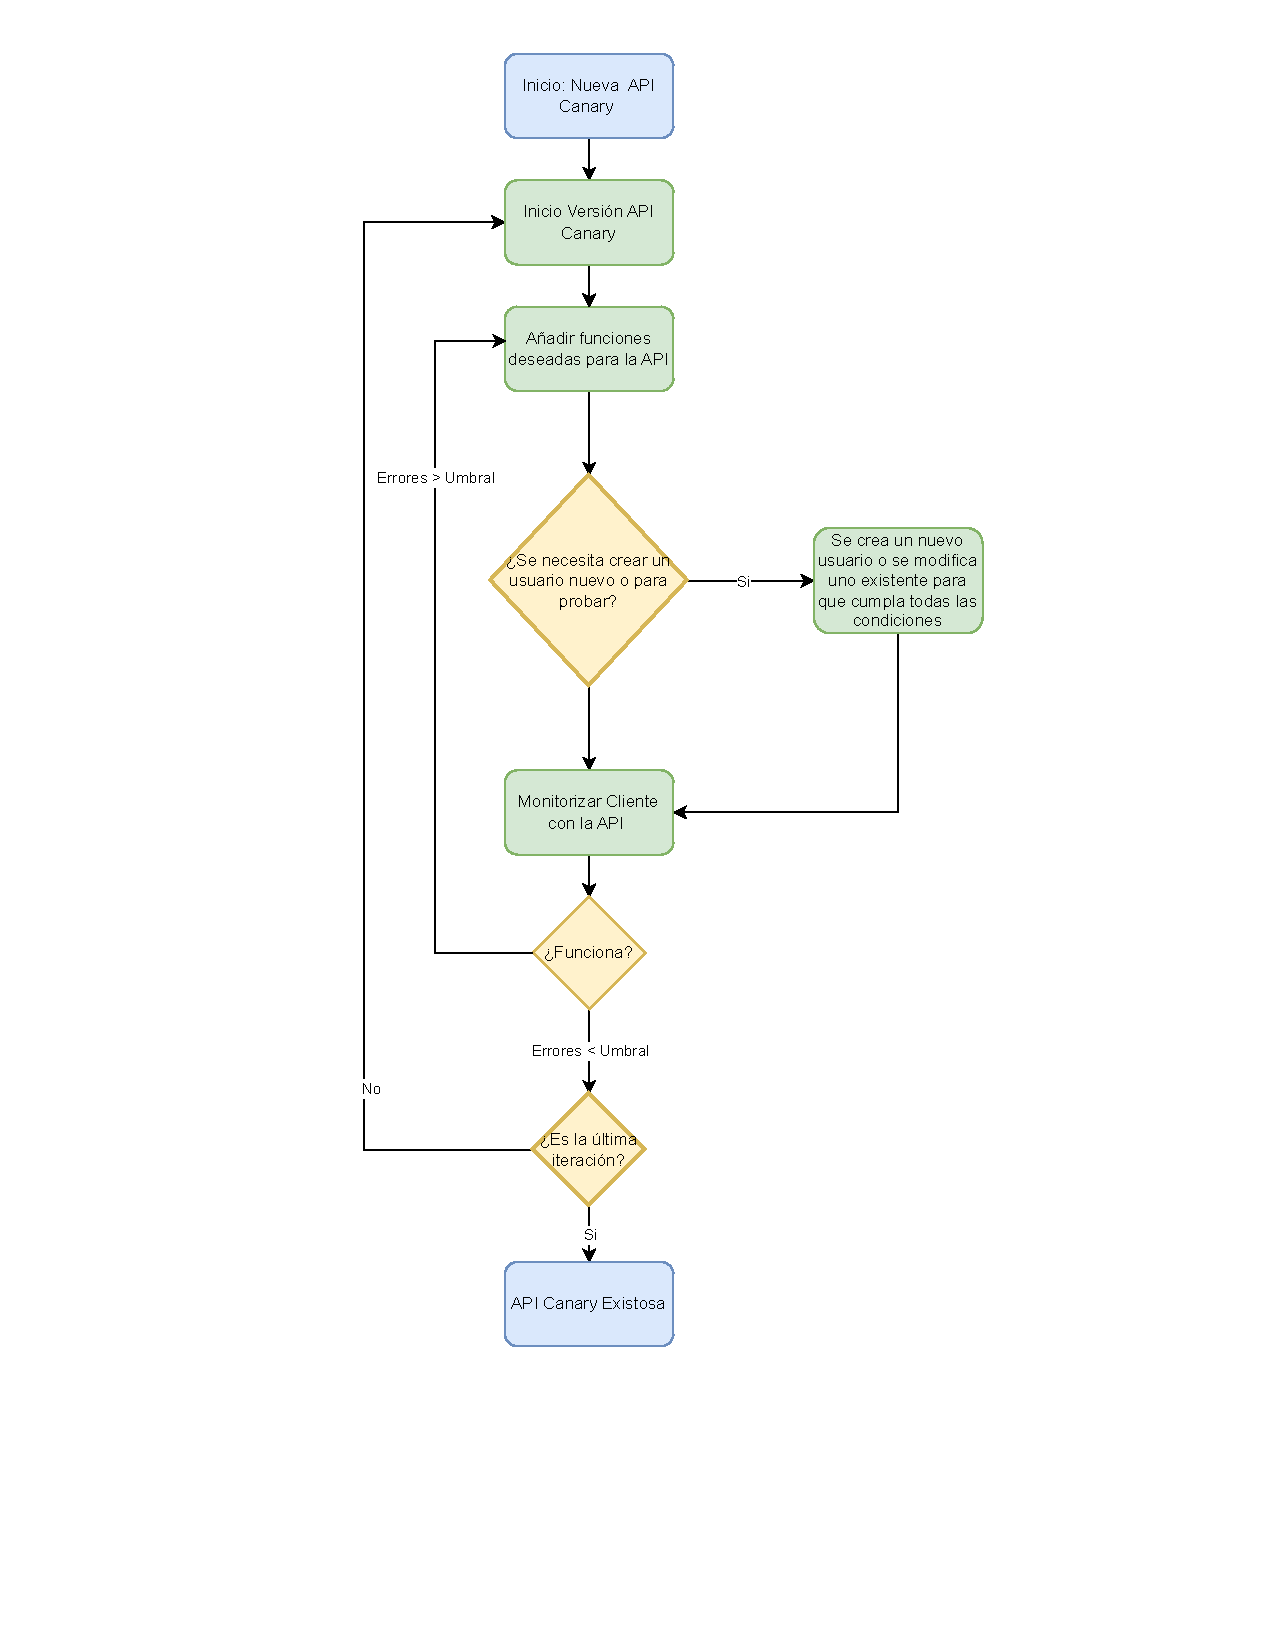
\includegraphics[width=0.9\textwidth]{archivos/flujo_API_Canary.drawio.pdf}
    \caption{Diagrama de flujo del proceso de despliegue Canary para APIs}
    \label{fig:canary-flow}
\end{figure}

\textbf{Descripción del flujo:}
\begin{enumerate}
    \item \textbf{Inicio: Nueva API Canary} - Desarrollo de una nueva API de validación.

    \item \textbf{Inicio: Nueva Versión API Canary} - Desarrollo de una nueva versión de la API de validación, en la que se inicia la nueva iteración.

    \item \textbf{Inicio: Añadir funciones deseadas} - Se implementan las nuevas funciones deseadas.

    \item \textbf{Comprobación de completitud del usuario de muestra} - Se comprueba que el usuario que se usa para comprobar el correcto funcionamiento de la API tiene todos los recursos necesarios que debe comprobar. En el caso contrario, se modifica para que permita comprobar todas las funciones a comprobar, en su defecto se creará un nuevo perfil para ello.

    \item \textbf{Monitorizar Métricas} - Análisis continuo de errores, latencia y otras métricas clave.

    \item \textbf{Decisión basada en umbrales:}
          \begin{itemize}
              \item \textbf{Si errores < Umbral} → Se pasa a la siguiente fase de la API.
              \item \textbf{Si errores > Umbral} → Rollback automático a versión estable y se revisan las actualizaciones para volver a modificar y lograr hacer funcionales los cambios.
          \end{itemize}

    \item \textbf{API Canary Exitosa} - Tras terminar todas las fases, se integra y entra la fase de automatizarla para que se ejecute periódicamente.
\end{enumerate}



% ===== SECCIÓN 1.4: TECNOLOGIAS Y HERRAMIENTAS =====

\section{Tecnologías y Herramientas Utilizadas}

\noindent Para el desarrollo del sistema de validación de facturación cloud, se ha construido una arquitectura tecnológica robusta que combina herramientas modernas de desarrollo, infraestructura contenerizada y patrones de diseño específicos para el dominio de facturación.

\subsubsection{Stack Tecnológico Principal}

\begin{table}[h!]
    \centering
    \begin{tabular}{|p{0.25\textwidth}|p{0.7\textwidth}|}
        \hline
        \textbf{Categoría}                         & \textbf{Tecnologías}                    \\
        \hline
        \hline
        \textbf{Runtime}                           & Node.js 18+ (LTS)                       \\
        \hline
        \textbf{Lenguaje}                          & JavaScript ES6+ con módulos             \\
        \hline
        \textbf{Framework Web}                     & Express.js con middleware personalizado \\
        \hline
        \textbf{Gestión de Paquetes}               & Yarn 3+ con workspace                   \\
        \hline
        \textbf{Testing}                           & Postman                                 \\
        \hline
        \textbf{Creación de usuarios de muestreo } & DCD de IONOS                            \\
        \hline
        \textbf{Base de Datos Configuración}       & CouchDB para configuración distribuida  \\
        \hline
        \textbf{Control de Versiones}              & GitLab para paquetes internos           \\
        \hline
        \textbf{Editor de Código}                  & Visual Studio Code                      \\
        \hline
        \textbf{Documentación}                     & LaTeX en OverLeaf                       \\
        \hline
        \textbf{Creación de diagramas}             & Draw.io                                 \\
        \hline
        \textbf{Conexión con equipo }              & VPN a red Alemana                       \\
    \end{tabular}
    \caption{Stack tecnológico del proyecto}
    \label{tab:stack-tecnologico}
\end{table}

\subsubsection{Dependencias Clave del Proyecto}

\textbf{Dependencias Internas:}
\begin{itemize}
    \item \texttt{@internal/core} - Framework base con utilidades de inicialización y configuración
    \item \texttt{@internal/dev} - Suite de herramientas para desarrollo y debugging
\end{itemize}

\textbf{Dependencias Externas Críticas:}
\begin{itemize}
    \item \texttt{helmet} - Middleware de seguridad para cabeceras HTTP
    \item \texttt{express} - Framework web minimalista para Node.js
    \item \texttt{couchdb-nano} - Cliente para integración con CouchDB
\end{itemize}

\subsubsection{Arquitectura Modular Implementada}

La arquitectura del sistema se organiza en tres capas principales:

\begin{enumerate}
    \item \textbf{Capa de Infraestructura:}
          \begin{itemize}
              \item CouchDB para gestión de configuración centralizada
          \end{itemize}

    \item \textbf{Capa de Servicios:}
          \begin{itemize}
              \item \texttt{data-api}: Servicio de acceso y transformación de datos
              \item \texttt{invoice-validation}: Motor de validación de facturación
              \item \texttt{utilization}: Procesamiento de métricas de uso
          \end{itemize}

    \item \textbf{Capa de Helpers y Utilidades:}
          \begin{itemize}
              \item Módulo \texttt{schema}: Validación y transformación de datos
              \item Módulo \texttt{actions}: Operaciones comunes del negocio
              \item Módulo \texttt{invoice}: Lógica específica de facturación
          \end{itemize}
\end{enumerate}

\subsubsection{Flujo de Desarrollo y Calidad}

\begin{itemize}
    \item \textbf{Desarrollo Local:} Nodemon para hot-reload durante el desarrollo
    \item \textbf{Calidad de Código:} ESLint con configuración personalizada
    \item \textbf{Control de Cambios:} Hooks pre-commit para validaciones automáticas
    \item \textbf{Integración:} Pipelines CI/CD en GitLab para despliegue continuo
\end{itemize}





\newpage

% ============================================
% ===== CAPÍTULO 3: ITERACIONES =====
% ============================================
\newpage
\chapter{Iteraciones}\label{chap:iteraciones}
\section{Primera Iteración}
\subsection{Planificación y Análisis}
Siendo esta la primera iteración, es en la que más se desarrolla para que en las siguientes iteraciones todo resulte más sencillo, como ya se había planeado adjudicandole más horas que al resto de iteraciones.
Esta iteración se basa en 4 puntos: la creación de la función para detectar los \textit{items} continuables;
las configuraciones iniciales en CouchDB; la creación de las primeras alarmas --- después de crearlas, solo habrá que modificar su contenido
en el resto de iteraciones --- y la creación del contrato.


\vspace{0.6cm}

Uno de los objetivos fundamentales de esta iteración es sentar las bases del proyecto y definir las tecnologías que se emplearán. Esto abarca tanto el lenguaje de programación como el sistema de control de versiones. En este caso, ambas decisiones son heredadas: se usa \textit{JavaScript} --- cumpliendo así el requisto RNF05 y el RNF09 --- porque es el lenguaje en el que están desarrolladas las librerías internas del equipo de Billing de IONOS Cloud, y para el versionado se utiliza GitLab de manera habitual. Además, por seguridad, el código se respalda periódicamente tanto en GitHub como en un disco duro físico, como se explicó en la sección \hyperref[sec:plan-contingencias]{Plan de contingencias y riesgos}.


\vspace{0.6cm}

Referido a la detección de los \textit{items} continuables, se realiza en dos fases: la primera consiste en detectar solamente un SKU concreto y, cuando funcione, se extiende al resto de SKUs.

\vspace{0.6cm}

Tanto la configuración inicial de CouchDB, como la creación de las alarmas y la formalización del contrato se abordan con especial atención al detalle. En el caso del contrato, esto implica verificar que todos los SKUs disponibles estén contemplados, ya que una cobertura completa desde el inicio evita tener que revisarlo en iteraciones posteriores. Además, tanto el contrato como las alarmas se diseñan siguiendo el principio de abierto/cerrado de los principios SOLID: preparados para incorporar futuras actualizaciones mediante la adición de nuevos elementos, sin necesidad de modificar el código existente.

\vspace{1cm}

\subsubsection{Verificación de SKUs con PostMan}
Para la verificación de los SKUs disponibles en la API de IONOS Cloud, hemos optado por utilizar
\textbf{PostMan}\Cite{PostMan-Learning} como herramienta de prueba y automatización. Antes de comenzar a utilizarlo, es
importante comprender su funcionamiento y las capacidades que ofrece para este proyecto.

PostMan es una plataforma de colaboración para el desarrollo de APIs que permite diseñar, probar,
documentar y monitorizar APIs de manera eficiente. Para este trabajo, aprovecharemos especialmente
su capacidad para ejecutar scripts de prueba en JavaScript y su sistema de colecciones que permite
automatizar peticiones.

\paragraph{Conceptos básicos de PostMan para la verificación de SKUs}

Antes de comenzar a usarlo, es importante entender algunos conceptos
clave de PostMan:

\begin{itemize}
    \item \textbf{Collections:} Son grupos de peticiones relacionadas que pueden organizarse en carpetas.
          En nuestro caso, crearemos una colección específica para las pruebas de verificación de SKUs de
          IONOS Cloud.

    \item \textbf{Environments y variables:} PostMan permite definir entornos con variables reutilizables.
          Utilizaremos variables de entorno para almacenar:
          \begin{itemize}
              \item La URL base de la API de IONOS Cloud.
              \item Los tokens de autenticación de forma segura.
              \item Los resultados de las verificaciones para su uso en otras peticiones.
          \end{itemize}

    \item \textbf{Pre-request scripts:} Scripts que se ejecutan \textit{antes} de enviar una petición.
          Nos permitirán preparar datos, generar tokens temporales o configurar cabeceras de autenticación
          automáticamente.

    \item \textbf{Tests scripts:} Scripts que se ejecutan \textit{después} de recibir la respuesta de la API.
          Aquí implementaremos la lógica de verificación de SKUs, comparando los recursos obtenidos con
          la lista predefinida de recursos requeridos.

    \item \textbf{Console:} Herramienta de depuración que muestra los logs generados por nuestros scripts.
          Utilizaremos \texttt{console.log()} para generar reportes detallados del estado de cada verificación.

    \item \textbf{Runner:} Funcionalidad que permite ejecutar colecciones completas de manera automática,
          ideal para realizar verificaciones periódicas sin intervención manual.
\end{itemize}

\subsubsection{Base de datos con CouchDB}
Para las configuraciones, exceptuando los tokens y las claves, se ha optado por utilizar \textbf{CouchDB}\Cite{CouchDB-Info}, para cumplir el requisito RNF10, una base de datos NoSQL
orientada a documentos que destaca por su facilidad de integración con aplicaciones web. Realizando esta tarea el 20 de febrero de 2026.

\paragraph{Características principales de CouchDB para el proyecto}

\begin{itemize}
    \item \textbf{Almacenamiento basado en JSON:} Los datos se guardan como documentos JSON, lo que
          facilita su manipulación desde aplicaciones JavaScript como la que estamos desarrollando.

    \item \textbf{API RESTful nativa:} CouchDB expone una API HTTP que permite realizar operaciones
          CRUD mediante peticiones estándar (GET, POST, PUT, DELETE), lo que simplifica tanto la comunicación con
          el backend como la integración con nuestro proyecto.

    \item \textbf{Replicación maestro-maestro:} Soporta sincronización bidireccional entre múltiples
          instancias, lo que facilita la distribución de datos y la tolerancia a fallos, aspecto relevante para cumplir el requisito RNF01.

    \item \textbf{MVCC (Multiversion Concurrency Control):} Utiliza control de concurrencia mediante
          versiones, evitando bloqueos en lecturas y escrituras simultáneas, ayudando a cumplir el requisito RNF01.
\end{itemize}




\subsection{Desarrollo y despliegue}

\subsubsection{Creación del contrato}
El requisito RF01.01 exige un usuario exclusivo para las pruebas, por lo que es necesario crear un contrato dedicado. Tras una breve investigación se concluyó que no existía un método sencillo para crearlo de forma automática; se optó por hacerlo manualmente, ya que el coste de tiempo era menor y el proceso más directo. La creación del contrato se inició el 15 de febrero y finalizó el 19 de febrero de 2026.

El método elegido combina el DCD de IONOS con comprobaciones periódicas en PostMan. Como paso previo hay que disponer de una cuenta de IONOS Cloud y darse de alta en el DCD; al tratarse de un proceso sencillo, no se detalla aquí ---si se desea más información, se puede consultar el \hyperref[anexo:crear-cuenta-token]{Anexo 2}---.

Al añadir los \textit{items} de la lista al contrato se completa el requisito RF02.01 y sus dependencias. Una vez incorporados, estos recursos permanecen activos todos los meses, lo que satisface ---para los \textit{items} continuables--- el requisito RF02.03: sin modificaciones, el consumo mensual será predecible y estable.

Previamente a la creación del contrato, se elaboró la lista de SKUs a detectar a partir de la documentación de IONOS Cloud~\cite{billing-IONOSCloud}. Inicialmente constaba de 52 SKUs ---con posibles incorporaciones posteriores en las iteraciones 4 y 5, al añadir los \textit{items} no continuables---. El resultado se recoge en el \hyperref[anexo:Lista-de-SKUs]{Anexo 1}, con los SKUs seleccionados teniendo en cuenta los requisitos RF01.03 y RNF04, y dando cumplimiento al requisito RF01.02. Dicha lista se completó el 6 de febrero de 2026, respetando las fechas establecidas.

\vspace{0.5cm}

El primer problema encontrado fue vincular los recursos a sus SKUs, ya que la denominación de algunos no es intuitiva. Para resolverlo se recurrió a la API interna de IONOS Cloud~\cite{billing-IONOSCloud}.

Para utilizar dicha API se necesitaba, además de la documentación, un token generado por el contrato ---la forma de obtenerlo es sencilla y no es objeto del proyecto; para más información véase el \hyperref[anexo:crear-cuenta-token]{Anexo 2}---. Una vez obtenido, resulta imprescindible crear un plan de uso y control de estos tokens, dado que constituyen información delicada.

\subsubsection{Plan de gestión de tokens de autenticación}
\label{iteraciones:gestion-tokens}
Para garantizar la seguridad en el acceso a la API de IONOS Cloud, se establece un plan de gestión de tokens de autenticación utilizando \textbf{KeePassXC} como gestor de contraseñas especializado, cumpliendo así el requisito RNF03.

\paragraph{Justificación de la herramienta}
\vspace{0.25cm} 
KeePassXC es un gestor de contraseñas de código abierto, auditado de forma independiente, que proporciona cifrado robusto (AES-256, Twofish o ChaCha20) para la información almacenada \cite{keepassxc-audit}. Entre sus características más relevantes para este proyecto destacan:
\begin{itemize}
    \item Capacidad de generar contraseñas y tokens seguros.
    \item Almacenamiento cifrado de secretos con protección en memoria.
    \item Generación integrada de TOTP (Time-based One-Time Passwords) \cite{keepassxc-features}.
    \item Compatibilidad con archivos clave y YubiKey para autenticación de doble factor.
    \item Integración con navegadores mediante extensiones oficiales.
\end{itemize}

\paragraph{Ciclo de vida de los tokens en IONOS Cloud}
\vspace{0.25cm}
Los tokens de autenticación en IONOS Cloud presentan las siguientes características \cite{ionos-token-management}:
\begin{itemize}
    \item Se generan a través del \textit{Authentication Token Manager} en el DCD.
    \item Cada token tiene un TTL (\textit{Time To Live}) configurable entre 1 hora y 365 días.
    \item El valor del token solo se muestra una única vez durante su generación.
    \item Es posible descargar el token como archivo de texto en el momento de creación.
    \item Se pueden generar hasta 100 tokens por cuenta.
    \item La eliminación de un token lo invalida inmediatamente, incluso antes de su fecha de expiración.
\end{itemize}

\paragraph{Procedimiento de gestión segura}
\vspace{0.25cm}
\begin{enumerate}
    \item \textbf{Generación del token:}
          \begin{itemize}
              \item Acceder al DCD: Menú → Management → Token Manager.
              \item Seleccionar TTL adecuado al caso de uso (para desarrollo: 30-90 días; para producción: evaluar periodicidad de rotación).
              \item Generar el token y, en la pantalla de visualización, seleccionar \textit{Download} para obtener el archivo de texto.
          \end{itemize}

    \item \textbf{Almacenamiento en KeePassXC:}
          \begin{itemize}
              \item Crear una entrada específica para cada token en la base de datos de KeePassXC.
              \item Campos a rellenar:
                    \begin{itemize}
                        \item \textbf{Título:} ``Token IONOS API - [Propósito]'' (ej: ``Token IONOS API - Desarrollo Iteración 1'').
                        \item \textbf{Nombre de usuario:} Identificador del token (Token ID).
                        \item \textbf{Contraseña:} Pegar el valor del token.
                        \item \textbf{URL:} https://api.ionos.com (para integración con navegador).
                        \item \textbf{Notas:} Fecha de generación, TTL seleccionado, fecha de expiración calculada, propósito específico.
                    \end{itemize}
              \item Adjuntar el archivo de texto descargado como archivo adjunto en la entrada.
              \item Configurar la entrada para generar TOTP si se requiere autenticación adicional.
          \end{itemize}

    \item \textbf{Rotación y expiración:}
          \begin{itemize}
              \item Configurar un recordatorio en el calendario para 7 días antes de la fecha de expiración.
              \item En la fecha de rotación:
                    \begin{enumerate}
                        \item Generar nuevo token en el DCD.
                        \item Almacenarlo en KeePassXC siguiendo el procedimiento anterior.
                        \item Eliminar el token antiguo desde el DCD.
                        \item Marcar la entrada antigua como expirada o eliminarla de la base de datos.
                    \end{enumerate}
          \end{itemize}

    \item \textbf{Seguridad adicional:}
          \begin{itemize}
              \item La base de datos de KeePassXC debe protegerse con una contraseña maestra robusta (mínimo 15 caracteres con alta entropía).
              \item Habilitar el bloqueo automático de la base de datos tras periodo de inactividad.
          \end{itemize}
\end{enumerate}

\subsubsection{Uso del Token}

Una vez definida la gestión de los tokens, estos se pueden utilizar para realizar llamadas a la API de facturación. En concreto, se emplea el endpoint \textit{"https://api.ionos.com/billing/\{contract\}/products"}~\cite{billing-IONOSCloud}, que devuelve la información de los productos asociados al contrato. De este modo es posible verificar la presencia de cada recurso deseado.

Para ejecutar estas llamadas se utiliza PostMan.
Como primer SKU a detectar se opta por A01000 (IP estática). Para ello se añade una IP estática de forma manual en el DCD y, tras pasar el periodo que tarda en actualizarse
la base de datos de la API, se hace una llamada y debe aparecer. En este caso debe salir algo similar a:

\begin{lstlisting}[caption=Ejemplo de producto en API de IONOS, label=lst:producto-json]
{
    "products": [
        {
            "meterId": "A01000",
            "meterDesc": "30d per static IP address",
            "deprecated": false,
            "unit": "30Days",
            "type": "consumption",
            "unitCost": {
                "quantity": "5",
                "unit": "EUR"
            }
        }
    ]
}
\end{lstlisting}

Realizar este proceso de forma manual ---tanto la verificación como la incorporación de productos--- resulta propenso a errores por su naturaleza repetitiva. Por ello, se opta por una solución más fiable y reutilizable: aprovechar la capacidad de PostMan para ejecutar scripts y crear uno que compruebe automáticamente si están presentes los SKUs deseados.

\subsubsection{Creación del script de verificación}
\label{iteraciones:script-verificacion-postman}

Se creó un script en JavaScript para PostMan que verifica los SKUs disponibles.

\paragraph{Funcionamiento}
\begin{enumerate}
    \item Define un objeto \texttt{requiredResources} con 14 categorías de SKUs (IPs estáticas, VMs, almacenamiento, bases de datos, etc.).
    \item La función \texttt{checkResources()} compara cada SKU requerido con los devueltos por la API.
          \begin{lstlisting}[label=lst:verificacion-categorias]
Object.keys(requiredResources).forEach(category => {
    const resources = requiredResources[category];
    results.available[category] = [];
    results.missing[category] = [];
    
    resources.forEach(resource => {
        const found = products.find(p => p.meterId === resource);
        if (found) { results.available[category].push(resource);
        } else { results.missing[category].push(resource); } }); });

\end{lstlisting}
    \item Clasifica los resultados en \texttt{available} (encontrados) y \texttt{missing} (no encontrados).
          \begin{figure}[h!]
              \centering
              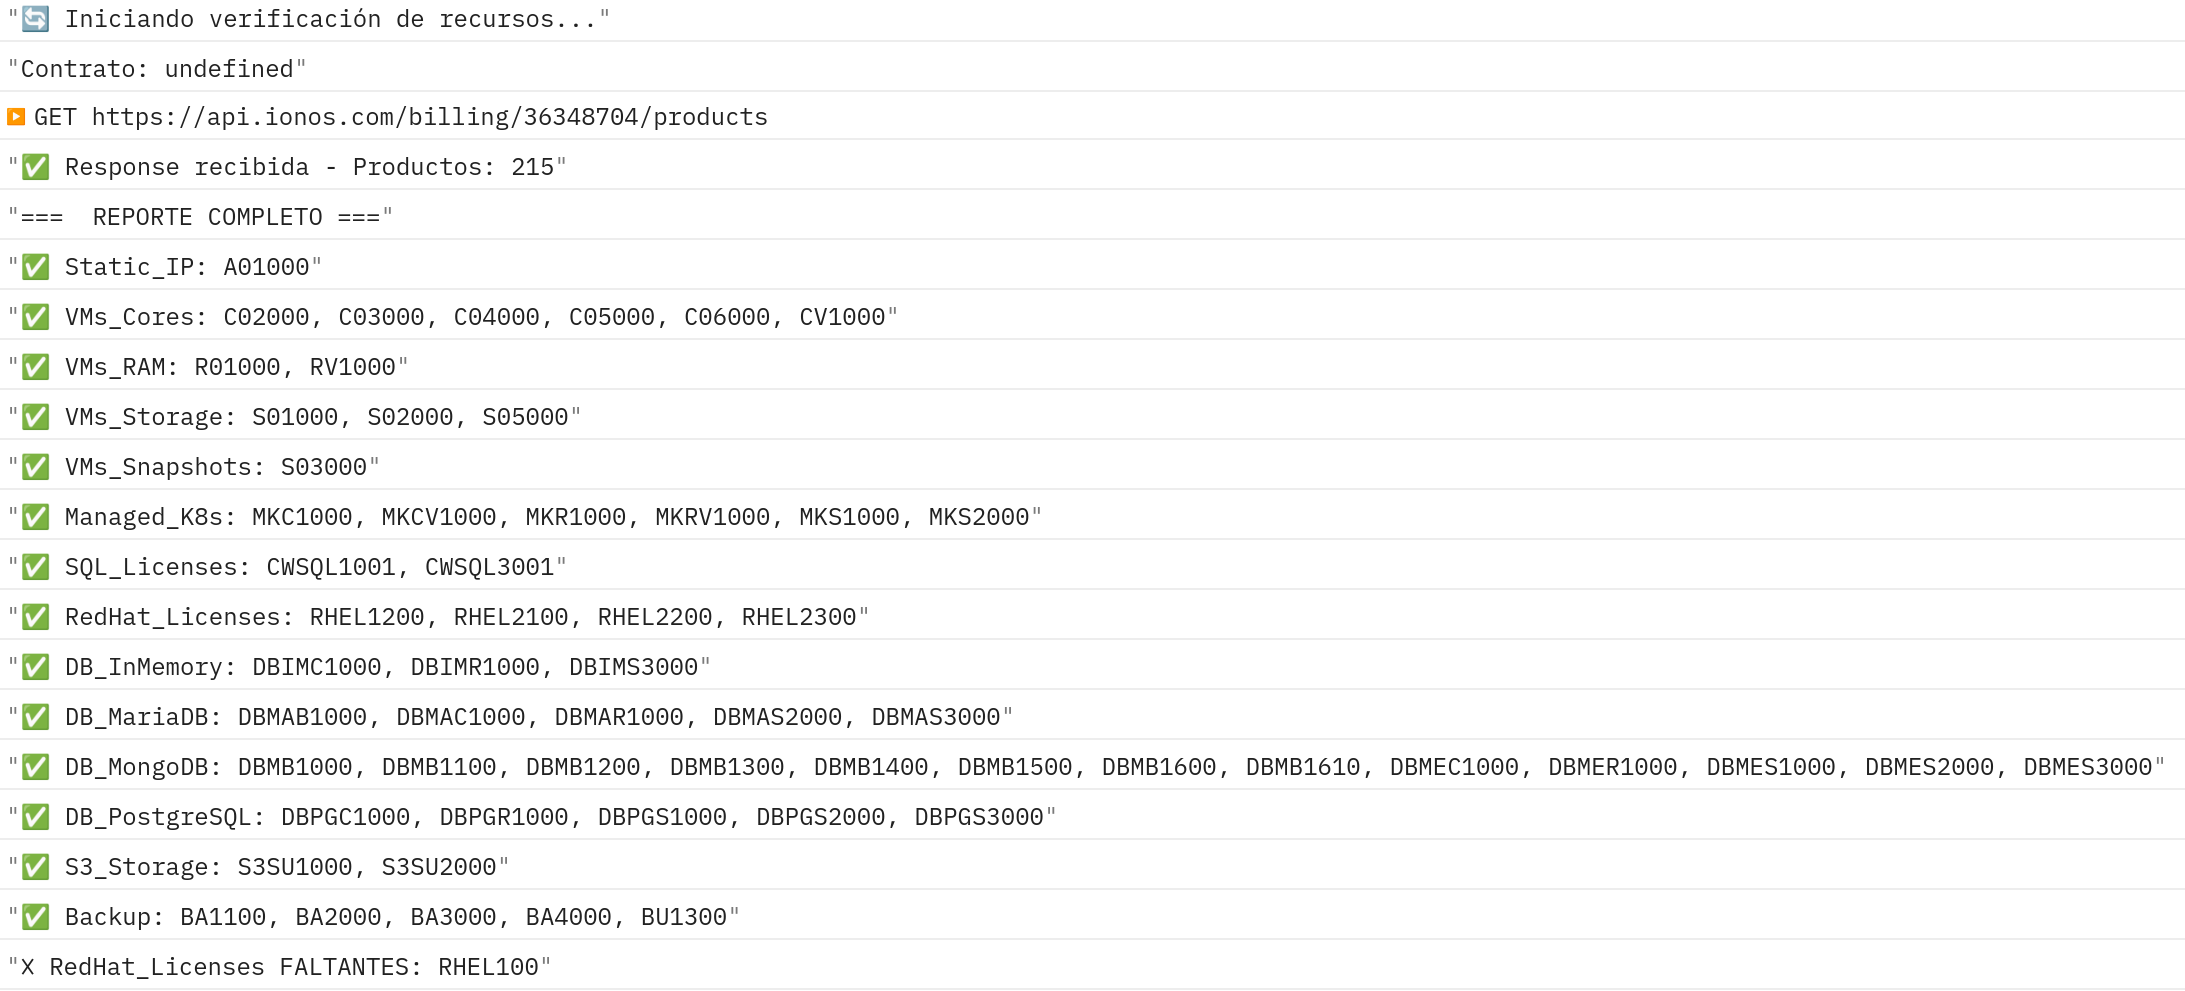
\includegraphics[width=1\textwidth]{PostMan-Test.png}
              \caption{Prueba Test}
              \label{fig:edt}
          \end{figure}
    \item Detecta patrones especiales: VMs CUBE (contienen ``CUBES'') y licencias Windows (empiezan por ``WL'').
    \item Almacena los resultados en variables de entorno de PostMan.
    \item Genera un reporte en consola con el estado de cada categoría.
    \item Calcula estadísticas globales: total disponibles vs total requeridos.
          \begin{figure}[h!]
              \centering
              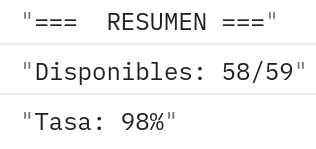
\includegraphics[width=0.25\textwidth]{PostMan-Resumen.png}
              \caption{Prueba Resumen Test}
              \label{fig:edt}
          \end{figure}
    \item Ejecuta tests automáticos (código 200, productos no vacíos).
          \begin{figure}[h!]
              \centering
              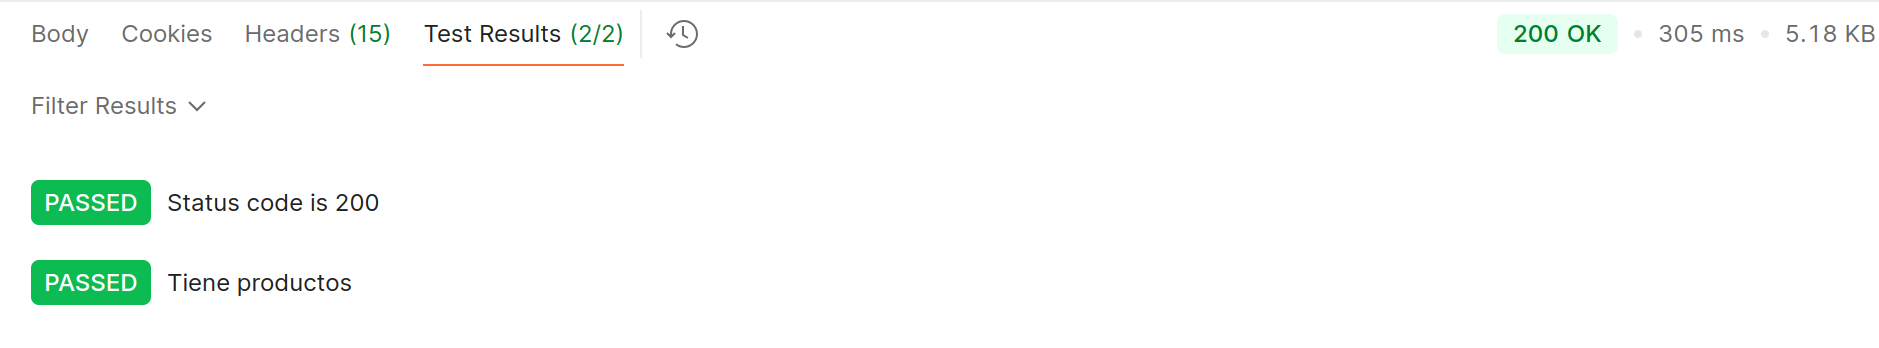
\includegraphics[width=0.7\textwidth]{PostMan-CodsOK.png}
              \caption{Prueba Cods. Test}
              \label{fig:edt}
          \end{figure}
\end{enumerate}

\paragraph{Ventajas}

Automatiza la verificación, proporciona trazabilidad, se integra en PostMan y es fácilmente mantenible. Además, esta estructura es migrable al proyecto, permitiendo tener una parte ya hecha.

\subsection{Integración del código}
\subsubsection{Configuración de Entornos}
Al ser la primera iteración se deben configurar los entornos que se van a usar.
Esto consiste en la creación del proyecto, su vinculación a GitLab y GitHub,
el plan de copias de seguridad en físico y la configuración inicial en CouchDB. Estas tareas son indispensables para cumplir los requisitos RNF10, RF02.02, RF04.03 y RF05.01.  
\subsubsection{Despliegue del proyecto y vinculación a GitLab}
El proyecto se crea directamente desde GitLab ---cumpliendo así el requisito RNF08--- porque se desea integrarlo en el grupo de trabajo del equipo de \textit{Cloud Billing} y \textit{ERP} de IONOS Cloud, de modo que, tras la finalización del proyecto, todo el equipo pueda continuar con su mantenimiento. Por este motivo se sigue, además, la estructura de proyectos propia del equipo. La única peculiaridad fue la necesidad de usar la VPN, ya que el GitLab empleado es el corporativo del equipo, alojado en Alemania.

\subsubsection{Estrategia de copias de seguridad del código fuente usando GitHub y disco físico}
Para garantizar la integridad y disponibilidad del código fuente desarrollado en este proyecto,
se ha establecido una estrategia de copias de seguridad multicapa que complementa el sistema de
control de versiones principal.

\paragraph{Uso de GitLab como sistema de control de versiones principal}
GitLab actúa como el repositorio principal donde se gestiona el desarrollo activo del proyecto.
Sus características incluyen:
\begin{itemize}
    \item Control de versiones con historial completo de cambios.
    \item Gestión de ramas para el desarrollo de funcionalidades.
    \item Integración continua para pruebas automáticas.
    \item Documentación integrada mediante wikis.
\end{itemize}

\paragraph{GitHub como repositorio espejo de respaldo}
A pesar de utilizar GitLab como plataforma principal, se ha configurado GitHub como repositorio
secundario para proporcionar una capa adicional de redundancia. Esta decisión se fundamenta en:

\begin{itemize}
    \item \textbf{Independencia entre plataformas:} Al estar alojados en servidores de diferentes
          proveedores, una caída o problema en GitLab no compromete el acceso al código.

    \item \textbf{Redundancia geográfica:} Los datos se replican en centros de datos de diferentes
          ubicaciones, protegiendo frente a desastres regionales. Esto previene uno de los posibles riesgos estudiados en el plan de riesgos.
\end{itemize}

\paragraph{Copia de seguridad en disco físico local}
Complementando las copias en la nube, se realiza una copia de seguridad periódica en un disco físico
externo siguiendo estos principios: 

\begin{itemize}
    \item \textbf{Frecuencia de respaldo:} Copia completa del repositorio cada 15 días y copia
          incremental de los cambios diarios.

    \item \textbf{Almacenamiento seguro:} El disco se mantiene en una ubicación física diferente a la
          del equipo de desarrollo, protegiendo frente a robo, incendio o fallo del equipo principal.

    \item \textbf{Verificación de integridad:} Tras cada backup, se ejecuta una comprobación automática
          mediante \texttt{git fsck} para garantizar que el repositorio no esté corrupto.
\end{itemize}

\subsubsection{Configuración en CouchDB}
Debido a que el proyecto está integrado en el grupo de trabajo de \textit{Cloud Billing} y \textit{ERP}, se utiliza su grupo de bases de datos. --- Cumpliendo así el requisito RNF10. ---
Lo único que hay que tener en cuenta es el uso de las credenciales; dado que las credenciales para acceder a CouchDB
son delicadas ---ya que se accede a todas las configuraciones del equipo---, se emplea un protocolo similar al descrito en la
sección \hyperref[iteraciones:gestion-tokens]{Plan de gestión de tokens de autenticación}.

Una vez creada la base de datos propia, se crea un documento para vincularlo con el proyecto.


\paragraph{Estructura del documento de configuración}
El documento almacenado en CouchDB contiene la lógica y parámetros necesarios para las verificaciones:

\begin{itemize}
    \item \textbf{Identificador:} \texttt{billing-reference-verifier} - Documento raíz que centraliza
          toda la configuración del verificador. Este nombre coincide con el del proyecto, estandarizado por el grupo de trabajo, lo que cumple parcialmente el requisito RNF09.

    \item \textbf{Programación de tareas (scheduler):} Define ejecuciones automáticas periódicas; sobre esto se desarrollará en mayor profundidad cuando se hable de ello en concreto.

\end{itemize}

\paragraph{Configuración específica para verificación de SKUs}
El módulo \texttt{utilization} contiene la lista de SKUs a monitorizar, siguiendo la siguiente estructura:

\begin{lstlisting}[caption=Almacenamiento SKUs en CouchDB, label=lst:producto-json]
{
    "skus_monitorizados": [
        "A01000", "C02000", "C03000", "C04000", "C05000", "C06000",
        [...],
        "CWSQL1001", "RHEL2100"
    ]
}
\end{lstlisting}
\subsubsection{Estructura general del proyecto billing-reference-verifier}

El proyecto \texttt{billing-reference-verifier} es una API REST interna desarrollada para IONOS
cuyo propósito principal es verificar la utilización de recursos y validar facturas asociadas a
contratos de facturación. Antes de abordar los detalles técnicos, se describe a continuación la estructura general del proyecto y las tecnologías que lo componen. Cumpliendo asi los requisitos RNF05, RNF06, RNF07 y  RNF09.

\paragraph{Información general}
\begin{itemize}
    \item \textbf{Nombre:} billing-reference-verifier
    \item \textbf{Tecnología:} Node.js (versión $\geq$ 18.0.0) con framework interno \texttt{@internal/core}
    \item \textbf{Tipo:} API REST interna
\end{itemize}

\paragraph{Arquitectura de directorios}
La estructura del proyecto se organiza de la siguiente manera:

\begin{verbatim}
billing-reference-verifier/
|-- package.json                  # Dependencias y scripts de Node.js
|-- README.md                     # Documentacion principal
|-- run.sh / start.sh             # Scripts de inicio del servicio
|-- config/
|   +-- nginx.conf                # Configuracion de proxy reverso
|-- docs/
|   |-- README.md                  # Documentacion adicional
|   +-- SUMMARY.md                 # Resumen de documentacion
|-- src/
|   |-- run.js                     # Punto de entrada (bootstrap)
|   |-- helpers/                    # Clases auxiliares y utilidades
|   |   |-- actions.js              # Constantes de eventos/acciones
|   |   |-- invoice.js              # Helper para operaciones de facturas
|   |   |-- schema.js               # Esquemas de validacion Joi
|   |   +-- utilization.js          # Helper para datos de utilizacion
|   +-- modules/                    # Modulos funcionales de la aplicacion
|       |-- utilization/
|           +-- index.js            # Logica de verificacion de utilizacion
+-- test/
    +-- test-usage-validate.js      # Pruebas automatizadas
\end{verbatim}

\paragraph{Componentes principales}

\paragraph{Punto de entrada (run.js)}
Realiza el bootstrap de la aplicación utilizando el framework \texttt{@internal/core}, carga la
configuración definida en \texttt{package.json} e inicializa el servidor y los módulos.

\paragraph{Módulos funcionales}
\begin{itemize}
    \item \textbf{utilization:} Verifica las cantidades diarias de uso frente a los valores
          esperados para los SKUs configurados.
\end{itemize}

\paragraph{Helpers}
\begin{itemize}
    \item \textbf{actions.js:} Define constantes para los eventos del mediador (como
          \texttt{APPLICATION\_RUN}, \texttt{UTILIZATION\_VERIFIER\_COMPLETE}, etc.).

    \item \textbf{schema.js:} Contiene esquemas Joi para validar las respuestas de la API
          (\texttt{invoiceSchema}, \texttt{utilizationSchema}, \texttt{usageSchema}).

    \item \textbf{utilization.js:} Implementa la clase \texttt{UtilizationHelper} para obtener
          datos de los endpoints \texttt{/utilization} y \texttt{/usage} de la API de facturación.
\end{itemize}

\paragraph{Endpoints REST disponibles}

\begin{itemize}
    \item \texttt{GET /data/v1/utilization/check/:contractId} --- Verifica la presencia de ítems configurados.
    \item \texttt{GET /data/v1/utilization/debug} --- Información de diagnóstico.
    \item \texttt{POST /data/v1/invoice/manual-test/:contractId} --- Test manual de validación.
\end{itemize}

\paragraph{Flujo de datos}

\begin{enumerate}
    \item Una petición HTTP llega al módulo \texttt{data-api}, que valida los headers (incluyendo
          el token Bearer).
    \item El mediador emite un evento al módulo correspondiente según el endpoint solicitado.
    \item El módulo utiliza los helpers para realizar llamadas a la \texttt{billing-api} de IONOS.
    \item Las respuestas se validan mediante los esquemas Joi definidos en \texttt{schema.js}.
    \item Se devuelve una respuesta JSON estructurada con el resultado, resumen y timestamp.
\end{enumerate}

\paragraph{Dependencias externas}
\begin{itemize}
    \item \textbf{@internal/core:} Framework base que proporciona servidor Koa, cliente REST y utilidades.
    \item \textbf{helmet:} Middleware de seguridad para cabeceras HTTP.
    \item \textbf{@internal/dev:} Herramientas de desarrollo (eslint, nodemon, etc.).
    \item \textbf{joi:} Validación de esquemas (integrado a través de @internal/core).
\end{itemize}

\paragraph{Patrones de diseño utilizados}
\begin{itemize}
    \item \textbf{Módulos desacoplados:} Cada módulo hereda de una clase \texttt{Module} base.
    \item \textbf{Mediator Pattern:} Comunicación entre módulos mediante eventos.
    \item \textbf{Factory Pattern:} Uso de \texttt{createHelper()} para instanciar helpers.
    \item \textbf{Dependency Injection:} Container para servicios.
    \item \textbf{Schema Validation:} Joi para validar estructuras de datos.
\end{itemize}

\paragraph{Autenticación }
Todas las peticiones requieren el header \texttt{Authorization: Bearer <token>}. Este token se
transmite a la \texttt{billing-api} de IONOS para autenticar las operaciones y se gestiona como ya se explicó en
\hyperref[iteraciones:gestion-tokens]{el plan de gestión de tokens de autenticación} y garantizar el cumplimiento del requisito RNF03.

\subsection{Implementación de función de Detección de items continuables}
Una vez definida la estructura del proyecto, el 21 de febrero se inicia la implementación de la función de detección de ítems continuables en el módulo \texttt{utilization}. Esta función realiza llamadas a la API de facturación para obtener los datos de utilización y compararlos con la lista de SKUs monitorizados en CouchDB, logrando así la primera parte del requisito RNF04.02.

Para ello se implementa la función \texttt{checkUtilization()}, basada en el script que se creó para PostMan ---explicado en la sección \hyperref[iteraciones:script-verificacion-postman]{Creación del script de verificación}---. Al igual que en PostMan, el desarrollo se realiza en dos fases: primero se detecta un SKU concreto y, una vez verificado su correcto funcionamiento, se extiende al resto de SKUs.

\paragraph{Validación de respuestas con Joi}

Para garantizar la integridad de los datos recibidos de la API de facturación, se ha implementado la validación de las respuestas mediante esquemas \texttt{Joi}, definidos en el helper \texttt{schema.js}. Esto permite detectar de forma temprana respuestas inesperadas o malformadas de la API, devolviendo un error controlado en lugar de propagar datos incorrectos al resultado de la verificación. Además se ha creado la verificación de todos los futuros datos necesarios, es decir, ahora solo se necesitan los datos de utilización, pero se ha creado la validación de las facturas y del uso para futuras iteraciones, lo que cumple el requisito RNF06.

El archivo \texttt{schema.js} define tres esquemas de validación, cada uno adaptado a un endpoint distinto de la API de facturación:

\begin{itemize}
    \item \textbf{\texttt{invoiceSchema}:} Valida las respuestas de facturas procedentes de NetSuite. Incluye la verificación del total facturado (unidad y cantidad), metadatos de la factura (fechas, identificadores de factura, contrato y cliente) y un array de \textit{datacenters}, cada uno con su ubicación, medidores y descuentos (\textit{rebates}). Un aspecto destacable es la validación del formato del identificador de factura mediante una expresión regular:
\end{itemize}

\begin{lstlisting}[caption=Validación del formato de invoiceId, label=lst:invoice-pattern]
metadata: joi.object({
    invoiceId: joi.string().pattern(/^GY\d+$/).required(),
    contractId: joi.string().required(),
    postingPeriod: joi.string().pattern(/^\d{4}-\d{2}$/).required()
    // ...
}).required()
\end{lstlisting}

Esto garantiza que el identificador de factura siga siempre el patrón esperado por el sistema, rechazando respuestas con formatos incorrectos. De forma similar, el \texttt{postingPeriod} se valida contra el formato \texttt{YYYY-MM}.

\begin{itemize}
    \item \textbf{\texttt{utilizationSchema}:} Valida las respuestas del endpoint \texttt{/utilization}, que es el utilizado en esta iteración para detectar los ítems continuables. La estructura es más compleja, ya que cada medidor incluye referencias UUID a recursos y servidores, tipo de recurso, rango de fechas y región geográfica. Un ejemplo representativo de la validación de un medidor:
\end{itemize}

\begin{lstlisting}[caption=Validación de un medidor en utilizationSchema, label=lst:utilization-meter]
meters: joi.array().items(
    joi.object({
        id: joi.string().uuid().required(),
        resourceId: joi.string().uuid().required().allow(null),
        serverId: joi.string().uuid().required().allow(null).allow(''),
        type: joi.string().required(),
        meterId: joi.string().required(),
        region: joi.string().required(),
        quantity: joi.object({
            quantity: joi.number().required(),
            unit: joi.string().required()
        }).required()
    }).required()
).required()
\end{lstlisting}

Es relevante el uso de \texttt{.allow(null)} y \texttt{.allow('')} en campos como \texttt{resourceId} y \texttt{serverId}, ya que no todos los recursos del DCD tienen un servidor o recurso físico asociado de forma directa, pero el campo debe estar presente en la respuesta. Sin esta flexibilidad, la validación rechazaría respuestas legítimas de la API.

\begin{itemize}
    \item \textbf{\texttt{usageSchema}:} Valida las respuestas del endpoint \texttt{/usage}, que se utilizará en iteraciones posteriores. Su estructura es más sencilla que la del esquema de utilización, pero incorpora un aspecto interesante: la cantidad puede venir como número o como cadena numérica, lo que se resuelve con \texttt{alternatives()}:
\end{itemize}

\begin{lstlisting}[caption=Validación flexible de cantidad en usageSchema, label=lst:usage-alternatives]
quantity: joi.object({
    quantity: joi.alternatives().try(
        joi.number(),
        joi.string().regex(/^\d+(?:\.\d+)?$/)
    ).required(),
    unit: joi.string().required()
}).required()
\end{lstlisting}

Esta flexibilidad es necesaria porque la API de facturación devuelve en ocasiones valores numéricos como cadenas de texto (por ejemplo, \texttt{"4.5"} en lugar de \texttt{4.5}), comportamiento que puede variar entre versiones o entre distintos tipos de recursos.

Los tres esquemas comparten un conjunto de validadores comunes de Joi: \texttt{required()} para campos obligatorios, \texttt{optional()} para opcionales, \texttt{pattern()} para expresiones regulares, \texttt{valid()} para valores permitidos (como \texttt{'EU'} y \texttt{'US'} en la ubicación de los datacenters), \texttt{uuid()} para identificadores universales y \texttt{array().items()} para validar arrays de objetos con estructura definida.

\subsubsection{Creación de endpoint y decisión de formato de URL}
Debido a que no hay ningún requisito que especifique el formato de la URL, se opta por un formato RESTful que refleje claramente la acción realizada. Se decide utilizar el endpoint \texttt{GET /data/v1/utilization/check/:contractId}, donde \texttt{contractId} es un parámetro dinámico que permite especificar el contrato para el cual se desea realizar la verificación de utilización. Este formato es intuitivo y sigue las convenciones REST, facilitando su comprensión y uso por parte de otros desarrolladores o sistemas que puedan integrarse con esta API en el futuro.
Sin embargo, no se puede garantizar que este formato se mantenga en el futuro, ya que no hay un requisito que lo especifique, por lo que podría cambiarse en futuras iteraciones si el cliente lo considera necesario. Por ello, se documenta claramente en el README del proyecto para asegurar que cualquier cambio futuro se realice de manera controlada y con conocimiento de las partes involucradas.


\subsection{Desarrollo e implementación}

La primera tarea llevada a cabo en esta primera iteración ha sido la configuración de los entornos necesarios para el desarrollo del sistema. Esta fase incluye principalmente el despliegue del proyecto en GitLab, la configuración de la base de datos CouchDB y su vinculación con el proyecto, y la preparación del entorno de pruebas mediante PostMan. Aunque también se han creado los repositorios de respaldo en GitHub y se ha configurado la VPN para acceder a la infraestructura corporativa, estas acciones se consideran triviales dentro del alcance técnico del proyecto.

\subsubsection{Configuración de PostMan}
Para la realización de pruebas sobre las peticiones HTTP a la API de facturación de IONOS Cloud, se ha configurado PostMan. La herramienta permite simular las llamadas que realizará el sistema de verificación, facilitando la creación y prueba de peticiones REST antes de integrarlas en el código.

Se han configurado los siguientes elementos:
\begin{itemize}
    \item \textbf{Collection:} Se ha creado una colección específica denominada \textit{billing-reference-verifier} para agrupar todas las peticiones de verificación.
    \item \textbf{Variables de entorno:} Se han definido variables para la URL base de la API de IONOS Cloud, el \texttt{contractId} de pruebas y el token de autenticación Bearer, evitando así tener que introducirlos manualmente en cada petición.
\end{itemize}

Es importante configurar correctamente los encabezados, el cuerpo de las peticiones según lo requiera cada endpoint de la API de facturación, ya que una configuración incorrecta puede provocar errores difíciles de diagnosticar.

Tras reunirse con el cliente, se sugerieron por su parte dos cambios, la primera el estandarizar el contrato y eliminarlo de la URL de la petición, denido a que siempre se usará el mismo contrato y en el caso de querer usar otro en el futuro se puede modificar en la configuración. La segunda fue usar desde PostMan \texttt{Authorization: Bearer <token>} en lugar de una variable personalizada, para que sea más fácil de usar y entender. Ambos cambios se implementarán en la proxima iteración.

%% TODO: Si quieres incluir el esquema Joi utilizado (utilizationSchema, usageSchema, etc.), añádelo aquí.


\subsubsection{Configuración de ejecución programada}

Para automatizar las verificaciones y cumplir el requisito RF04.01, se ha configurado un \textit{scheduler} en el documento de CouchDB que define la periodicidad de ejecución de las comprobaciones.

%% TODO: Añadir aquí los detalles concretos del scheduler: frecuencia (diaria, semanal, etc.),
%% formato de la configuración en CouchDB y cómo se dispara la ejecución (cron job, servicio interno, etc.).

De esta forma, el sistema realiza verificaciones de manera autónoma sin necesidad de intervención manual, generando alertas únicamente cuando se detectan discrepancias.

\subsection{Pruebas y validación}

Para verificar el correcto funcionamiento de la iteración se han diseñado pruebas a dos niveles: pruebas manuales con PostMan y pruebas automatizadas integradas en el proyecto.

\subsubsection{Pruebas manuales con PostMan}

Se han ejecutado peticiones al endpoint \texttt{GET /data/v1/utilization/check/:contractId} desde PostMan, verificando que:
\begin{itemize}
    \item La respuesta devuelve un código 200 cuando la petición es correcta.
    \item Todos los SKUs de la lista se encuentran en la categoría \texttt{available}.
    \item La respuesta incluye la estructura esperada: \texttt{result}, \texttt{summary} y \texttt{timestamp}.
    \item Al eliminar un recurso del contrato de pruebas de forma temporal, el SKU correspondiente aparece en la categoría \texttt{missing} y se dispara la alerta configurada.
\end{itemize}


\subsubsection{Pruebas automatizadas}

Se han implementado pruebas automatizadas en el archivo \texttt{test/test-usage-validate.js} que verifican la correcta validación de los esquemas Joi frente a las respuestas de la API. El enfoque elegido consiste en definir dos muestras de datos ---una válida y otra inválida--- y comprobar que el esquema acepta la primera y rechaza la segunda.

La muestra válida reproduce una respuesta real del endpoint \texttt{/usage}, con un datacenter de ubicación \texttt{EU}, un medidor con SKU \texttt{A01000} (IP estática) y una cantidad expresada como cadena numérica (\texttt{"0.87"}), lo que permite verificar simultáneamente la estructura general y el comportamiento del validador \texttt{alternatives()} descrito anteriormente:

\begin{lstlisting}[caption=Muestra válida para el test de validación, label=lst:valid-sample]
const validSample = {
    startDate: '2025-11-01',
    endDate: '2025-11-26',
    datacenters: [{
        id: 'a786c097-d6a6-531c-a55d-6e72ce4c35c5',
        name: '',
        location: 'EU',
        meters: [{
            meterId: 'A01000',
            meterDesc: '30d per static IP address',
            quantity: { quantity: '0.87', unit: '30Days' }
        }]
    }],
    metadata: { customerId: '117048209', contractId: '036348704' }
};
\end{lstlisting}

La muestra inválida introduce intencionadamente dos errores: una cantidad con un valor no numérico (\texttt{"not-a-number"}) y la ausencia del campo obligatorio \texttt{contractId} en los metadatos. De este modo se comprueba que el esquema detecta tanto errores de formato como campos ausentes:

\begin{lstlisting}[caption=Muestra inválida para el test de validación, label=lst:invalid-sample]
const invalidSample = {
    // ...misma estructura...
    meters: [{
        meterId: 'A01000',
        meterDesc: '30d per static IP address',
        quantity: { quantity: 'not-a-number', unit: '30Days' }
    }],
    metadata: { customerId: '117048209' } // contractId ausente
};
\end{lstlisting}

Las aserciones se realizan con el módulo estándar \texttt{assert} de Node.js, verificando que la validación de la muestra válida no produzca errores y que la muestra inválida sí los genere:

\begin{lstlisting}[caption=Aserciones del test, label=lst:test-assertions]
const { error: vError } = usageSchema.validate(validSample, { convert: true });
assert.strictEqual(vError, undefined, 'validSample should pass');

const { error: iError } = usageSchema.validate(invalidSample, { convert: true });
assert(iError, 'invalidSample should fail');
\end{lstlisting}

La opción \texttt{convert: true} permite que Joi transforme automáticamente los tipos cuando sea posible (por ejemplo, cadenas de fecha a objetos \texttt{Date}), simulando así el comportamiento real del sistema en producción. El test se ejecuta mediante \texttt{node test/test-usage-validate.js} y devuelve un código de salida 0 en caso de éxito o 1 en caso de fallo, lo que facilita su integración en pipelines CI/CD.


\subsection{Configuración de alertas}

Para cumplir los requisitos RF05.01 y RF05.02, se ha implementado un sistema de notificaciones que se dispara cuando la verificación detecta SKUs ausentes. En esta primera iteración, la alerta informa de los SKUs que no han sido encontrados en el contrato, permitiendo al equipo actuar de forma inmediata.

La configuración de alertas definitiva se realizará utilizando la infraestructura propia del equipo de Billing y ERP. Sin embargo, al tratarse de una primera iteración, se ha optado por una solución provisional más sencilla: el envío de notificaciones mediante \textit{webhooks} de Google Chat. Este mecanismo permite enviar mensajes a un espacio de Google Chat mediante una simple petición HTTP POST a una URL generada por la propia plataforma, sin necesidad de configurar servicios intermedios ni gestionar autenticación adicional.

El contenido de la alerta incluye:


Esta solución es suficiente para las primeras fases del proyecto, ya que permite al equipo recibir notificaciones en tiempo real sin un coste de implementación elevado. En la Figura~\ref{fig:alerta-iteracion1} se muestra un ejemplo de alerta recibida en Google Chat durante esta iteración.

\begin{figure}[H]
    \centering
    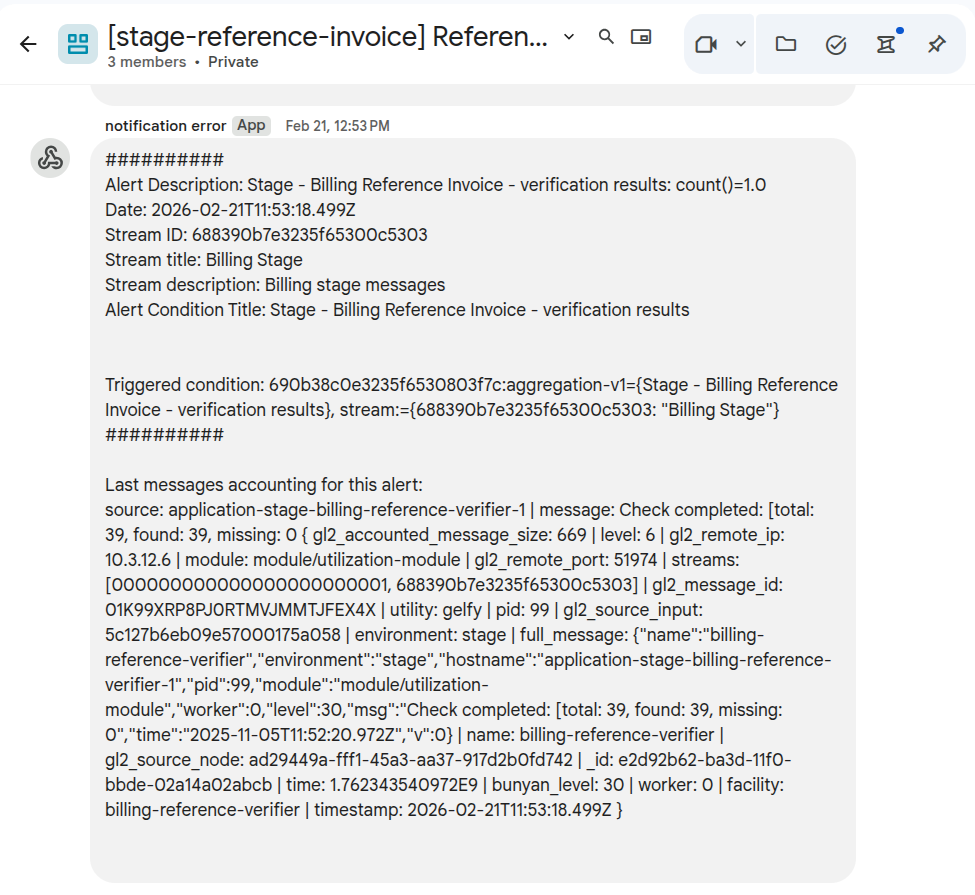
\includegraphics[width=0.8\textwidth]{Alerta1Iteracion.png}
    \caption{Ejemplo de alerta de la primera iteración recibida en Google Chat}
    \label{fig:alerta-iteracion1}
\end{figure}

En iteraciones posteriores, cuando se integre el sistema de alertas del equipo, bastará con sustituir la llamada al webhook por el mecanismo correspondiente, sin modificar la lógica de detección que genera el contenido de la alerta.

\subsection{Conclusiones de la iteración}

Tras finalizar esta primera iteración el 26 de febrero de 2026, me reuní con el cliente para revisar los resultados obtenidos y planificar los siguientes pasos. Se verificó que la función de detección de ítems continuables funciona correctamente, identificando tanto los SKUs presentes como los ausentes en el contrato de pruebas. Además, se confirmó que las alertas se generan y envían a Google Chat según lo esperado. Quedan pendientes para la próxima iteración los cambios sugeridos por el cliente en relación con las peticiones.

En cuanto a la planificación temporal, aunque la iteración se ha finalizado antes de lo previsto ---debido a los márgenes del plan de contingencias y a que se han invertido más horas semanales de las planificadas---, las horas totales dedicadas se han aproximado bastante a la estimación inicial. 

\begin{table}[H]
    \centering
    \begin{tabular}{|l|c|c|c|}
        \hline
        \textbf{Tarea} & \textbf{Estimadas (h)} & \textbf{Reales (h)} & \textbf{Desviación}\\ 
        \hline
        Detección de items continuables & 16h & 16h & 0\% \\
        Creación de contrato completo & 12h & 16h & +25\% \\
        Configuración de credenciales & 6h & 4h & -33.3\% \\
        Testeo de funcionamiento & 4h & 4h & 0\% \\
        Configuración de alertas y rutinas & 4h & 2h & -50\% \\
        \hline
        \textbf{Total} & \textbf{42h} & \textbf{42h} & \textbf{0\%} \\
        \hline
    \end{tabular}
    \caption{Comparativa de horas estimadas vs reales en la Iteración 1}
    \label{tab:horas-iteracion1}
\end{table}


\section{Iteración 2}
\subsection{Planificación}
En esta iteración se trabajará principalmente en ampliar las funcionalidades del sistema de verificación, evolucionando desde la simple detección de existencia de SKUs hacia la verificación de cantidades de uso. Además, se implementarán las mejoras solicitadas por el cliente durante la revisión de la primera iteración.

\textbf{Verificación de cantidades de uso:} En la iteración anterior se implementó la detección de existencia de SKUs (\texttt{existence-only}). Ahora se ampliará esta funcionalidad para verificar que las cantidades de uso reportadas por la API coincidan con los valores esperados. Esto permitirá detectar anomalías como recursos que reportan menos cores, RAM o almacenamiento del esperado. Además de ser el preambulo final para lograr el requisito RF04.02. 

\textbf{Sistema de thresholds:} Se implementará un sistema de umbrales configurable que permita distinguir entre situaciones de \textit{warning} (desviación menor) y \textit{error} (desviación crítica), adaptándose a las diferentes tolerancias según el tipo de recurso.

\textbf{Cambios solicitados por el cliente:} Se implementarán los dos cambios sugeridos en la reunión de cierre de la iteración anterior. Por un lado, estandarizar el contrato eliminándolo de la URL del endpoint ---ya que siempre se utilizará el mismo contrato de pruebas y, si se desea cambiar en el futuro, se modificará en la configuración de CouchDB---. Por otro lado, modificar PostMan para utilizar \texttt{Authorization: Bearer <token>} de forma estándar, mejorando la claridad y facilitando el uso por parte de otros miembros del equipo.


\subsection{Análisis} 

\subsubsection{Tipos de verificación: existence-only vs precise}
Tras analizar los diferentes SKUs monitorizados, se identifican dos categorías de verificación necesarias:

\begin{itemize}
    \item \textbf{existence-only:} Para recursos cuyo consumo puede variar legítimamente (IPs estaticas, Bases de datos). En estos casos, basta con verificar que existe consumo mayor que cero, sin comparar contra un valor esperado concreto.
    
    \item \textbf{precise:} Para recursos con cantidades fijas y predecibles (cores de CPU, GB de RAM). Estos requieren calcular el valor esperado y compararlo con el reportado por la API, aplicando umbrales de tolerancia para detectar discrepancias.
\end{itemize}

Por ejemplo, el SKU \texttt{C05000} (cores de CPU) tiene un valor base de 8 cores que debe mantenerse constante, mientras que \texttt{MKS1000} (almacenamiento en Kubernetes) solo requiere verificar que existe consumo.

\subsubsection{Sistema de thresholds}
Para los SKUs con verificación \texttt{precise}, se definen dos niveles de alerta basados en el ratio entre el valor real y el esperado:

\begin{itemize}
    \item \textbf{Warning:} Se activa cuando el ratio cae por debajo del umbral de warning (típicamente 0.99). Indica una desviación menor que requiere atención pero no es crítica.
    
    \item \textbf{Error:} Se activa cuando el ratio cae por debajo del umbral de error (típicamente 0.975). Indica una discrepancia significativa que requiere acción inmediata.
\end{itemize}

Estos umbrales son configurables por SKU en CouchDB, permitiendo ajustar la sensibilidad según las características de cada recurso. Ya que hay recursos como los cores de CPU donde una desviación del 1\% puede ser relevante, mientras que en otros como el almacenamiento en Kubernetes, la mera ausencia de consumo es suficiente para generar una alerta.

\subsubsection{Estandarización del contrato en la configuración}
Actualmente, el \texttt{contractId} se pasa como parámetro en la URL del endpoint (\texttt{/check/:contractId}). Tras analizar los casos de uso previstos, se concluye que el sistema operará siempre sobre un único contrato de referencia, por lo que tiene sentido centralizar este valor en la configuración del scheduler de CouchDB.

Es importante aclarar que el contrato no se elimina del endpoint en ningún momento. Sin embargo, en los endpoints de chequeo, test y debug (\texttt{/check}, \texttt{/test}, \texttt{/debug}) se omitirá el parámetro \texttt{contractId} de la URL, ya que estos endpoints utilizarán siempre el contrato de pruebas configurado en CouchDB. En cambio, para el resto de endpoints se mantiene el \texttt{contractId} como parámetro en la URL, permitiendo así modificar fácilmente el contrato objetivo sin necesidad de alterar la configuración almacenada en la base de datos.

\subsection{Desarrollo y pruebas}

\subsubsection{Configuración de itemsToCheck en CouchDB}
Se ha ampliado la estructura de configuración del módulo \texttt{utilization} en CouchDB para soportar ambos tipos de verificación. Cada ítem ahora incluye:

\begin{lstlisting}[caption=Estructura de itemsToCheck en CouchDB, label=lst:items-to-check]
{
    "itemsToCheck": [
        {
            "sku": "C05000",
            "value": 8,
            "verification": "precise",
            "calculationType": "cpu-hours",
            "thresholds": {
                "warning": 0.99,
                "error": 0.975
            }
        },
        {
            "sku": "MKS1000",
            "verification": "existence-only"
        }
    ]
}
\end{lstlisting}

Esta estructura permite definir de forma declarativa qué verificación aplicar a cada SKU, facilitando la adición de nuevos recursos sin modificar el código.

\subsubsection{Endpoint de verificación de cantidades diarias}
Se ha creado un nuevo endpoint específico para la verificación de cantidades diarias:

\begin{verbatim}
GET /data/v1/utilization/check-daily-quantity/:contractId
\end{verbatim}

Este endpoint realiza el siguiente proceso interno:
\begin{enumerate}
    \item Calcula los días transcurridos en el período de facturación actual.
    \item Obtiene los datos de uso desde la billing-api mediante \texttt{/\{contractId\}/usage}.
    \item Agrega el consumo por SKU utilizando la función \texttt{aggregateUsageData()}.
    \item Compara los valores actuales contra los esperados para cada SKU configurado.
\end{enumerate}

\subsubsection{Cálculo del valor esperado}
Para los SKUs con verificación \texttt{precise}, el valor esperado se calcula mediante la fórmula:

\begin{equation}
\texttt{expected} = \texttt{value} \times 24 \text{ horas} \times \texttt{días\_transcurridos}
\end{equation}

Donde \texttt{value} es el valor base configurado (por ejemplo, 8 cores) y \texttt{días\_transcurridos} son los días desde el inicio del período de facturación hasta ayer.

\subsubsection{Agregación de datos de uso}
La función \texttt{aggregateUsageData()} procesa la respuesta de la billing-api y agrupa el consumo por SKU:

\begin{lstlisting}[caption=Función de agregación de datos de uso, label=lst:aggregate-usage]
function aggregateUsageData(usageData) {
    const aggregated = {};
    usageData.datacenters.forEach(dc => {
        dc.meters.forEach(meter => {
            const sku = meter.meterId;
            if (!aggregated[sku]) {
                aggregated[sku] = 0;
            }
            aggregated[sku] += parseFloat(meter.quantity.quantity);
        });
    });
    return aggregated;
}
\end{lstlisting}

\subsubsection{Verificación y comparación}
La función \texttt{processItemVerification()} determina el tipo de verificación a aplicar:

\begin{lstlisting}[caption=Lógica de verificación por tipo, label=lst:process-verification]
if (itemConfig.verification === 'existence-only') {
    return this.generateExistenceVerification(sku, actualValue);
}
// Para verificacion precise:
const expected = itemConfig.value * 24 * daysElapsed;
const ratio = (actualValue / expected) * 100;
return this.evaluateWithThresholds(sku, actualValue, expected, ratio);
\end{lstlisting}

\subsubsection{Respuesta del endpoint}
El endpoint devuelve una respuesta estructurada con el resultado de cada verificación:

\begin{lstlisting}[caption=Ejemplo de respuesta del endpoint de cantidades diarias, label=lst:response-daily]
{
  "ok": true,
  "message": "daily-quantities check completed",
  "contractId": "36348704",
  "period": "this month until yesterday (3 days)",
  "daysCalculated": 3,
  "results": [
    {
      "sku": "C05000",
      "status": "ok",
      "actual": 1920.00,
      "expected": 1920.00,
      "ratio": 100,
      "calculationMethod": "precise"
    }
  ],
  "summary": {
    "total": 10,
    "ok": 8,
    "warnings": 1,
    "errors": 1
  }
}
\end{lstlisting}

El campo \texttt{ratio} se expresa como porcentaje, donde 100 indica coincidencia perfecta entre el valor actual y el esperado.

\subsubsection{Configuración de PostMan con Bearer Token estándar}
Se ha actualizado la colección de PostMan para utilizar la pestaña \textit{Authorization} con tipo \texttt{Bearer Token} en lugar de una variable personalizada en los headers. Este cambio:

\begin{itemize}
    \item Aprovecha la interfaz nativa de PostMan para gestión de tokens.
    \item Permite heredar la autenticación a nivel de colección, evitando configurarla en cada petición.
    \item Facilita el uso por parte de otros miembros del equipo que estén familiarizados con PostMan.
\end{itemize}

\subsubsection{Scheduler para verificación de cantidades diarias}
Se ha configurado un nuevo thread en el scheduler de CouchDB específico para la verificación de cantidades:

\begin{lstlisting}[caption=Configuración del scheduler para cantidades diarias, label=lst:scheduler-quantities]
{
    "thread": "utilization-verifier:daily-quantities",
    "enabled": true,
    "mutex": true,
    "timeout": 3600000,
    "action": "utilization-verifier:daily-quantities:request",
    "endAction": "utilization-verifier:daily-quantities:complete"
}
\end{lstlisting}

Este scheduler puede programarse con expresiones cron independientes del verificador de existencia, permitiendo ejecutar las verificaciones de cantidades con una frecuencia diferente si fuera necesario.



\subsection{Evaluación y reunión con el cliente}
Los cambios solicitados por el cliente se han implementado correctamente, simplificando el uso de la API y mejorando la configuración de PostMan. Además al volver a reunirme con el cliente dio el visto bueno a la iteración y hablamos sobre un posible cambio en el futuro de seprarar las credenciales de las configuraciones en dos documentos/formatos distintos, siendo este comentario más orientado a el grupo de trabajo entero que a mi trabajo, ya que esta decisión es propia del equipo de trabajo.

Referido a los tiempos, ocurre algo similar a la iteración anterior, se han finalizado antes de lo previsto, pero las horas totales dedicadas se han aproximado bastante a la estimación inicial. La desviación en la tarea de implementación de la verificación de cantidades se debe principalmente a la complejidad añadida por el sistema de thresholds y la necesidad de realizar pruebas adicionales para validar los diferentes escenarios (valores dentro del umbral de warning, valores que superan el umbral de error, etc.).

En resumen, la variación en los tiempos de esta iteración se debe a que fue necesario emplear tiempo adicional para implementar las mejoras solicitadas por el cliente, como el sistema de thresholds, la estandarización del contrato, el uso de Bearer Token en PostMan y la mejora del sistema de alertas. Esta complejidad añadida implicó realizar pruebas adicionales para validar diferentes escenarios (valores dentro del umbral de warning, valores que superan el umbral de error, etc.). Sin embargo, gracias a que las pruebas y la validación se simplificaron por estas mismas mejoras, el tiempo total invertido no se vio muy afectado, manteniéndose próximo a la estimación inicial y finalizándose antes de lo previsto.
Además de que se decidio desglosar y plasmar también el tiempo de reunión con el cliente, ya que aunque es una tarea que no aporta valor directo al desarrollo, es necesaria para la correcta evolución del proyecto y para garantizar que se cumplen las expectativas del cliente, por lo que se considera relevante incluirla en la comparativa de horas.

\begin{table}[H]
    \centering
    \begin{tabular}{|l|c|c|c|}
        \hline
        \textbf{Tarea} & \textbf{Estimadas (h)} & \textbf{Reales (h)} & \textbf{Desviación}\\
        \hline
        Verificación cantidades & 16h & 18h & +12.5\% \\
        Comprobación contrato completo & 1h & 10' & -83.3\% \\
        Configuraciones & 2h & 6h 10min & +205\% \\
        Pruebas y validación & 4h & 1h & -75\% \\
        Reunión con el cliente & 0h & 1h & $\infty$\% \\
        \hline
        \textbf{Total} & \textbf{24h} & \textbf{26h} & \textbf{+8.3\%} \\
        \hline
    \end{tabular}
    \caption{Comparativa de horas estimadas vs reales en la Iteración 2}
    \label{tab:horas-iteracion2}
\end{table}

% ============================================
% ===== TERCERA ITERACIÓN =====
% ============================================
\newpage
\section{Iteración 3}

\subsection{Planificación}

En esta iteración se cierra el ciclo de verificación de los \textit{items} continuables iniciado en las iteraciones anteriores: conocida la existencia de los SKUs (\textbf{TFG 3.1.1}) y verificadas sus cantidades de uso (\textbf{TFG 3.2.1}), el siguiente paso natural es contrastar el coste económico teórico con el importe real reflejado en la factura de IONOS Cloud (\textbf{TFG 3.3.1}).

\textbf{Comprobación del gasto de ítems continuables:} A partir de las cantidades de uso obtenidas de la \textit{billing-api} y de las tarifas unitarias configuradas en CouchDB, se calcula el importe esperado para cada SKU y se contrasta con el valor real de la factura. Este proceso resulta fundamental para satisfacer los requisitos RF03.01, RF03.02 y RF03.04, cuya ejecución está también vinculada al requisito RF04.02.

\textbf{Obtención y validación de la factura:} Se consume el endpoint de facturas de la API de IONOS Cloud y se valida la respuesta mediante el esquema Joi definido en iteraciones anteriores, asegurando que únicamente se procesan facturas cerradas y definitivas (\texttt{finallyPosted === true}).

\textbf{Sistema de tolerancias:} Se reutiliza y extiende el sistema de umbrales configurables implementado en la iteración anterior, añadiendo parámetros específicos para la validación de importes monetarios y \textit{rebates}.

Como en las iteraciones precedentes, se repiten las tareas transversales: verificación de completitud del contrato (\textbf{TFG 3.3.2}), actualización de credenciales y configuración en CouchDB (\textbf{TFG 3.3.3}), pruebas de funcionamiento (\textbf{TFG 3.3.4}) y configuración de alertas y rutinas (\textbf{TFG 3.3.5}).

\subsection{Análisis}

\subsubsection{Obtención de la factura real}

La \textit{billing-api} expone dos endpoints para el acceso a los datos de facturación:

\begin{enumerate}
    \item \textbf{Listado de facturas:} \texttt{GET /\{contractId\}/invoices} --- Devuelve la lista básica de facturas disponibles con su identificador y período de facturación.
    \item \textbf{Detalle de factura:} \texttt{GET /\{contractId\}/invoices/\{invoiceId\}} --- Devuelve la factura completa con el desglose por \textit{datacenter} y SKU.
\end{enumerate}

Los campos más relevantes de la respuesta son:

\begin{itemize}
    \item \textbf{\texttt{metadata.postingPeriod}:} Período de facturación en formato \texttt{YYYY-MM}.
    \item \textbf{\texttt{metadata.finallyPosted}:} Booleano que indica si la factura está cerrada y definitiva.
    \item \textbf{\texttt{total.quantity} / \texttt{total.unit}:} Importe total de la factura.
    \item \textbf{\texttt{datacenters[].meters[]}:} Desglose por SKU, con los campos \texttt{meterId}, \texttt{quantity}, \texttt{rate} y \texttt{amount}.
    \item \textbf{\texttt{datacenters[].rebate.amount.quantity}:} Descuento aplicado por \textit{datacenter}.
\end{itemize}

El verificador trabaja siempre sobre el \textbf{mes anterior cerrado}: se calcula el período del mes anterior y se busca en el listado la factura cuyo campo \texttt{date} coincida. El campo \texttt{finallyPosted} no está disponible en el endpoint de listado, por lo que se comprueba tras obtener el detalle completo de la factura mediante una llamada separada a \texttt{getInvoiceById()}. Si la factura aún no está disponible o \texttt{finallyPosted} es \texttt{false}, el proceso finaliza sin generar alertas, ya que podría seguir modificándose durante los primeros días del mes.

\subsubsection{Cálculo del coste teórico}

La fórmula de cálculo es directa. Para cada SKU se multiplica la cantidad de uso reportada por la tarifa unitaria almacenada en CouchDB bajo la clave \texttt{skuPrices}:

\begin{equation}
    \texttt{expectedAmount} = \texttt{expectedQuantity} \times \texttt{expectedRate}
\end{equation}

La tarifa \texttt{expectedRate} es independiente de la que figura en la factura. Esto es una decisión de diseño deliberada: si los precios de la factura contuviesen algún error, usar esa misma fuente para calcular el valor de referencia invalidaría cualquier detección de anomalía. Al mantenerla separada en CouchDB, el sistema conserva una fuente de verdad propia.

Las unidades se utilizan tal cual, sin conversiones adicionales: si la tarifa está expresada en EUR/30Days, la cantidad de uso vendrá igualmente en esas unidades.

\subsubsection{Sistema de tolerancias y estados}

Se extiende el sistema de umbrales de la iteración anterior con parámetros específicos para la validación de cantidades e importes. Los valores por defecto, configurables por SKU en CouchDB bajo \texttt{config.invoiceValidation.validationTolerances}, son los siguientes:

\begin{table}[H]
    \centering
    \begin{tabular}{|p{0.40\textwidth}|p{0.18\textwidth}|p{0.35\textwidth}|}
        \hline
        \textbf{Parámetro} & \textbf{Valor por defecto} & \textbf{Descripción} \\
        \hline
        \hline
        \texttt{DEFAULT\_QUANTITY\_TOLERANCE} & 1\% (0,01) & Tolerancia general de cantidad \\
        \hline
        \texttt{DEFAULT\_ERROR\_THRESHOLD} & 95\% (0,95) & Ratio mínimo para no generar error en cantidades \\
        \hline
    \end{tabular}
    \caption{Parámetros de tolerancia para validación de facturas}
    \label{tab:tolerancias-factura}
\end{table}

La lógica de estados difiere según el tipo de comparación:

\begin{itemize}
    \item \textbf{Validación de cantidades} (\texttt{calculateQuantityComparison}): tres estados posibles según el ratio respecto al valor esperado.
    \begin{itemize}
        \item \textbf{\texttt{ok}:} ratio $\geq$ 0,99 --- coincidencia prácticamente perfecta.
        \item \textbf{\texttt{warning}:} 0,95 $\leq$ ratio $<$ 0,99 --- desviación menor, requiere atención.
        \item \textbf{\texttt{error}:} ratio $<$ 0,95 --- discrepancia crítica, requiere acción inmediata.
    \end{itemize}
    \item \textbf{Validación de importes monetarios} (\texttt{validateAmounts}): únicamente dos estados: \textbf{\texttt{ok}} si el importe está dentro del umbral configurado, \textbf{\texttt{error}} en caso contrario. No existe estado intermedio \texttt{warning} para importes.
\end{itemize}

\subsection{Desarrollo y pruebas}

\subsubsection{Obtención y validación de la factura}

El primer paso del proceso es localizar la factura correspondiente al mes anterior cerrado. Para ello se utiliza el helper \texttt{InvoiceHelper}, que encapsula las llamadas a la \textit{billing-api}. El endpoint de listado devuelve únicamente metadatos básicos — entre ellos el campo \texttt{date} con el período — pero \textbf{no incluye \texttt{finallyPosted}}. Por ello, la búsqueda inicial filtra solo por \texttt{date}; la comprobación de \texttt{finallyPosted} se realiza tras obtener el detalle completo con \texttt{getInvoiceById()}:

\begin{lstlisting}[caption=Obtención de la factura del mes anterior cerrado, label=lst:get-invoice]
const targetPeriod = now.clone().subtract(1, 'month')
                                .startOf('month')
                                .format('YYYY-MM');

// NOTE: The list endpoint does NOT include finallyPosted,
// so we must fetch details to check it.
const invoices       = await invoiceHelper.listInvoices(contractId, token);
const matchingInvoice = invoices.find((inv) => inv.date === targetPeriod);
\end{lstlisting}

Si no se localiza ninguna factura para ese período, o si tras obtener el detalle \texttt{finallyPosted} es \texttt{false}, el verificador termina sin generar alertas. A continuación se valida la respuesta mediante \texttt{invoiceSchema} antes de continuar con el procesamiento. De este modo se garantiza que los campos esperados están presentes y con el formato correcto, evitando errores de acceso en etapas posteriores.

\subsubsection{Cálculo del coste teórico por SKU}

Con la factura validada se recorre el array de \textit{datacenters} y sus \textit{meters}. Para cada SKU se calcula el importe esperado y se determina si la diferencia absoluta respecto al importe real queda dentro de la tolerancia configurada:

\begin{lstlisting}[caption=Cálculo del importe esperado y validación de la desviación, label=lst:expected-amount]
const expectedRate    = skuPrices[meter.meterId];
const expectedAmount  = expectedQuantity * expectedRate;
const invoiceAmount   = parseFloat(meter.amount.quantity);

const difference      = invoiceAmount - expectedAmount;
const toleranceAmount = Math.abs(expectedAmount) * DEFAULT_QUANTITY_TOLERANCE;
const isValid         = Math.abs(difference) <= Math.max(toleranceAmount, REBATE_TOLERANCE);
\end{lstlisting}


\subsubsection{Validación de \textit{rebates}}

Los descuentos por \textit{datacenter} se validan de forma independiente al resto de la jerarquía, usando una tolerancia absoluta de 0,01. Esta tolerancia es más estricta en términos absolutos que la tolerancia porcentual de los SKUs, dado que los \textit{rebates} son importes fijos y pequeñas diferencias de redondeo son esperables en su cálculo:

\begin{lstlisting}[caption=Validación del rebate por datacenter, label=lst:rebate]
const rebateDiff   = Math.abs(actualRebate - expectedRebate);
const rebateStatus = rebateDiff < REBATE_TOLERANCE
    ? 'ok'
    : 'error';
\end{lstlisting}

\subsubsection{Endpoint de validación y ejecución programada}

Se ha añadido un endpoint de prueba manual que permite lanzar la validación sobre un contrato concreto sin esperar a la ejecución programada:

\begin{verbatim}
POST /data/v1/invoice/manual-test/:contractId
\end{verbatim}

Este endpoint devuelve una respuesta estructurada con el resultado por SKU, por grupo de producto y el estado global del contrato, lo que facilita la depuración y la revisión puntual de facturas.

Para la ejecución automática se ha añadido un nuevo \textit{thread} al \textit{scheduler} de CouchDB. El verificador corre los días 3, 4 y 5 de cada mes a las 14:00 (Europe/Berlin), dando margen para que la factura del mes anterior esté cerrada y disponible. La opción \texttt{mutex: true} garantiza que no se ejecutan dos instancias en paralelo si una tarda más de lo esperado:

\begin{lstlisting}[caption=Configuración del scheduler para validación de facturas, label=lst:scheduler-invoice]
{
    "thread":    "invoice-verifier:monthly",
    "enabled":   true,
    "mutex":     true,
    "timeout":   3600000,
    "action":    "invoice-verifier:monthly:request",
    "endAction": "invoice-verifier:monthly:complete"
}
\end{lstlisting}

Esta configuración satisface los requisitos RF04.01 (ejecución programada del sistema de validación) y RF03.04 (programación de \textit{jobs} cron), ya que el ciclo mensual encaja con la periodicidad de las facturas de IONOS Cloud.

\subsubsection{Comprobación de completitud del contrato (TFG 3.3.2)}

Como en las iteraciones anteriores, antes de comenzar con el desarrollo de la funcionalidad principal se verifica que el contrato de pruebas sigue conteniendo todos los SKUs necesarios (\textbf{TFG 3.3.2}). En este caso no fue necesario añadir ningún elemento nuevo, ya que los SKUs monitorizados no habían variado respecto a la iteración anterior.

\subsubsection{Actualización de credenciales y configuración (TFG 3.3.3)}

Se actualizó el documento de configuración de CouchDB para incluir los nuevos parámetros de tolerancia de facturación (\textbf{TFG 3.3.3}): \texttt{validationTolerances}, \texttt{skuPrices} y la configuración del nuevo \textit{thread} del \textit{scheduler}. La estructura de credenciales no requirió cambios adicionales, ya que el helper \texttt{InvoiceHelper} reutiliza los mismos tokens de acceso definidos en iteraciones previas.

\subsubsection{Pruebas manuales con PostMan (TFG 3.3.4)}

Se añadieron nuevas colecciones en PostMan para la validación de facturas (\textbf{TFG 3.3.4}), verificando los siguientes escenarios:

\begin{itemize}
    \item Respuesta 200 cuando la factura del mes anterior está disponible y finalizada.
    \item Estado global \texttt{ok} cuando todos los importes coinciden dentro del umbral configurado.
    \item Paso a \texttt{error} de un SKU concreto al introducir una tarifa incorrecta en \texttt{skuPrices} de CouchDB que supera la tolerancia configurada (la validación de importes solo produce \texttt{ok} o \texttt{error}, sin estado intermedio).
    \item Finalización sin alertas cuando \texttt{finallyPosted === false}, comprobando que el sistema espera a que la factura esté cerrada.
\end{itemize}

\subsubsection{Configuración de alertas (TFG 3.3.5)}

Se adaptó el sistema de alertas para incluir el nuevo verificador de facturas (\textbf{TFG 3.3.5}). Las alertas generadas siguen la misma estructura que las de iteraciones anteriores: se notifica el estado global del contrato y, en caso de \texttt{warning} o \texttt{error}, se detallan los SKUs y \textit{datacenters} afectados junto con el ratio calculado. Esto permite al equipo de operaciones identificar rápidamente si la discrepancia corresponde a un SKU concreto, a un grupo de producto o a un \textit{rebate} incorrecto.

\subsection{Evaluación}

En esta iteración se ha implementado la validación económica completa de los \textit{items} continuables, cerrando el ciclo de verificación que comenzó en la iteración 1 (detección de existencia de SKUs) y se amplió en la iteración 2 (verificación de cantidades de uso). El sistema puede ahora comparar el gasto teórico calculado con el importe real facturado, desglosándolo de forma jerárquica por SKU, grupo de producto y \textit{datacenter}, y generando alertas diferenciadas por nivel de criticidad.

Con esta iteración quedan satisfechos los requisitos \textbf{RF03.01} (cálculo del coste esperado por SKU), \textbf{RF03.02} (comparación con el importe real de la factura), \textbf{RF03.04} (programación de la ejecución mediante cron) y \textbf{RF04.02} (contraste entre el cálculo teórico y los datos reales de la API).

En esta reunión no fue necesaria la reunión con el cliente, ya que los cambios introducidos en esta iteración fueron pequeños y con la comunicación de los cambios y el modo en los que se hicieros via mensaje fue suficiente y no se requirió reunión. 

Referido a tiempos, se realizo según lo previsto aproximadamente, invirtiendo las horas necesarias, necesitanto menos tiempo para comprobar que el contrato estaba compledo debido a que no se introdujeron ningún cambio.

\begin{table}[H]
    \centering
    \begin{tabular}{|l|c|c|c|}
        \hline
        \textbf{Tarea} & \textbf{Estimadas (h)} & \textbf{Reales (h)} & \textbf{Desviación} \\
        \hline
        Comprobación gasto \textit{items} continuables & 16h & 16h & 0\% \\
        Comprobación contrato completo & 1h & 10' & -83\% \\
        Configuración de credenciales, alertas y rutinas & 2h & 2h y 30' & +25\% \\
        Testeo de funcionamiento & 4h & 4h & 0\% \\
        \hline
        \textbf{Total} & \textbf{23h} & \textbf{22h y 40'} & \textbf{3\%} \\
        \hline
    \end{tabular}
    \caption{Comparativa de horas estimadas vs reales en la Iteración 3}
    \label{tab:horas-iteracion3}
\end{table}

% ============================================
% ===== CUARTA ITERACIÓN =====
% ============================================
\newpage
\section{Iteración 4}

\subsection{Planificación}

Las tres iteraciones anteriores han completado el ciclo de verificación de los \textit{items} continuables: se detecta su presencia en el contrato, se contrasta su consumo diario y se valida su coste en la factura mensual. En esta cuarta iteración el foco cambia: se abordan por primera vez los \textit{items} no continuables, representados por los tokens de IA de IONOS Cloud (\textbf{TFG 3.4.1}).

A diferencia de los recursos de infraestructura (cores de CPU, RAM o almacenamiento), el consumo de tokens de IA solo existe si el sistema realiza llamadas activas al endpoint de inferencia. Sin generación controlada, la API de facturación simplemente no reflejaría consumo para los SKUs \texttt{AIL370I1100} (tokens de entrada) y \texttt{AIL370O1100} (tokens de salida), haciendo imposible cualquier verificación.

\textbf{Módulo generador de tokens:} Se implementará un módulo \texttt{generator} que, activado diariamente por el \textit{scheduler}, realice llamadas repetidas al endpoint de IA de IONOS Cloud hasta acumular un número mínimo de tokens configurable (\texttt{targetTokens}). El diseño sigue el mismo patrón basado en eventos ya utilizado en módulos anteriores.

\textbf{Control mediante configuración:} Todos los parámetros relevantes (modelo, \texttt{targetTokens}, \textit{prompt} y URL del endpoint) se centralizan en CouchDB, de modo que pueden ajustarse sin modificar el código.

\subsection{Análisis}

\subsubsection{El problema de los \textit{items} no continuables}

Los \textit{items} continuables ---como los cores de CPU o los GB de RAM--- generan consumo de forma automática mientras los recursos están activos. Los tokens de IA, en cambio, solo aparecen en la factura si se realizan llamadas explícitas al modelo. Esto plantea un problema de verificabilidad: sin consumo no hay datos que verificar, y sin generación controlada no es posible predecir cuántos tokens deberían aparecer.

La solución adoptada es crear un generador que se ejecute a hora fija cada día y produzca un volumen de tokens conocido de antemano. Una vez que el consumo es predecible, el módulo de verificación de utilización puede comprobar los SKUs de IA con verificación \texttt{existence-only}: basta con confirmar que hay consumo mayor que cero en el período.

\subsubsection{Separación de tokens de entrada y salida}

La API de IONOS Cloud distingue dos SKUs para el consumo de IA:

\begin{itemize}
    \item \textbf{\texttt{AIL370I1100}} (tokens de entrada / \textit{input}): corresponde a los tokens del \textit{prompt} enviado al modelo en cada llamada.
    \item \textbf{\texttt{AIL370O1100}} (tokens de salida / \textit{output}): corresponde a los tokens generados por el modelo en la respuesta.
\end{itemize}

Con un \texttt{targetTokens} de 100.000, la distribución habitual es aproximadamente 10.000 de entrada y 90.000 de salida, es decir, 0,01M y 0,09M respectivamente en las unidades de facturación. El \textit{prompt} largo es intencionado: cuanto más extenso sea, más tokens de salida genera el modelo por llamada, reduciendo el número de iteraciones necesarias para alcanzar el objetivo.

\subsubsection{Compatibilidad con el SDK de OpenAI}

El endpoint de inferencia de IONOS Cloud implementa la misma interfaz que la API de OpenAI, lo que permite utilizar el SDK oficial de Node.js (\texttt{openai}) apuntando a la URL del servicio de IONOS. La única diferencia respecto a un uso convencional del SDK es que \texttt{baseURL} apunta al endpoint de IONOS en lugar del de OpenAI, por lo que no fue necesario aprender ni integrar ningún cliente adicional.

El uso de \texttt{temperature: 0} garantiza respuestas deterministas: con el mismo \textit{prompt} y el mismo modelo, el número de tokens generados es reproducible entre ejecuciones, lo que facilita la predicción del consumo mensual acumulado.

\subsection{Desarrollo y pruebas}

\subsubsection{Configuración del \textit{scheduler} en CouchDB}

El generador se activa cada día a las 08:00 mediante un nuevo \textit{thread} en el \textit{scheduler}. La opción \texttt{mutex: true} impide que dos ejecuciones se solapen si la generación tarda más de lo habitual:

\begin{lstlisting}[caption=Configuración del scheduler para el generador de tokens, label=lst:scheduler-generator]
{
    "thread":    "generator",
    "enabled":   true,
    "mutex":     true,
    "timeout":   3600000,
    "action":    "generator:request",
    "endAction": "generator:complete",
    "schedule":  [["0 8 * * *", {}]]
}
\end{lstlisting}

El campo \texttt{action} debe coincidir exactamente con el nombre del evento registrado en el módulo, ya que es la cadena que el \textit{mediator} usa para enrutar el disparo.

\subsubsection{Módulo Generator: registro del evento}

El módulo \texttt{generator} sigue el mismo patrón que los módulos anteriores: en su método \texttt{init()} registra un \textit{listener} sobre el evento correspondiente y delega toda la lógica en el \textit{helper} especializado:

\begin{lstlisting}[caption=Registro del evento en el módulo Generator, label=lst:generator-event]
// src/modules/generator/index.js:22
this.mediator.on(Actions.GENERATOR_REQUEST, async () => {
    const result = await this.inferenceHelper.generateTokens();
    this.mediator.emit(Actions.GENERATOR_COMPLETE); // libera el mutex
});
\end{lstlisting}

La constante \texttt{Actions.GENERATOR\_REQUEST} vale \texttt{'generator:request'}, que coincide exactamente con el \texttt{action} configurado en el \textit{scheduler}. La emisión de \texttt{GENERATOR\_COMPLETE} al finalizar, independientemente del resultado, es lo que libera el \textit{mutex} y permite que la siguiente ejecución programada pueda arrancar.

\subsubsection{InferenceHelper: carga de configuración}

Antes de iniciar la generación, \texttt{InferenceHelper} lee sus parámetros desde CouchDB. Si alguno no está definido, aplica un valor por defecto:

\begin{lstlisting}[caption=Carga de parámetros de configuración en InferenceHelper, label=lst:inference-config]
// src/helpers/inference.js:35-39
const { baseUrl, apiKey, model, targetTokens, prompt }
    = this.getConfig().config || {};

this.targetTokens = targetTokens || 100000;
this.prompt       = prompt       || DEFAULT_PROMPT;
\end{lstlisting}

El \texttt{DEFAULT\_PROMPT} es un texto extenso sobre computación en la nube que actúa como \textit{fallback}. Su longitud es deliberada: un \textit{prompt} largo produce más tokens de salida por llamada, reduciendo el número de iteraciones necesarias para alcanzar \texttt{targetTokens}.

\subsubsection{InferenceHelper: bucle de generación}

El núcleo del módulo es un bucle que acumula tokens hasta superar el umbral configurado. En cada iteración se realiza una única llamada al modelo y se suman los tokens consumidos, separando los de entrada de los de salida:

\begin{lstlisting}[caption=Bucle de generación de tokens hasta alcanzar el objetivo, label=lst:inference-loop]
// src/helpers/inference.js:59
while (inputTokens + outputTokens < this.targetTokens) {
    const response = await this.client.chat.completions.create({
        model:       this.model,
        temperature: 0,
        messages:    [{ role: 'user', content: prompt }]
    });
    inputTokens  += response.usage.prompt_tokens     || 0;
    outputTokens += response.usage.completion_tokens || 0;
    calls++;
}
return { inputTokens, outputTokens,
         totalTokens: inputTokens + outputTokens, calls };
\end{lstlisting}

Con \texttt{targetTokens = 100.000} y un \textit{prompt} suficientemente largo, en la práctica suelen necesitarse una o dos llamadas para alcanzar el objetivo. Un resultado típico sería \texttt{\{inputTokens: 10000, outputTokens: 90000, totalTokens: 100000, calls: 1\}}.

\subsubsection{Actualización del contrato y configuración de verificación}

Los SKUs \texttt{AIL370I1100} y \texttt{AIL370O1100} son nuevos en el contrato, por lo que fue necesario añadirlos. A diferencia de los SKUs continuables, se configuran con verificación \texttt{existence-only}: no se compara contra un valor esperado fijo, sino que basta con confirmar que hay consumo mayor que cero, ya que la cantidad exacta puede variar ligeramente según el número de días transcurridos en el período:

\begin{lstlisting}[caption=Configuración de los SKUs de IA en itemsToCheck, label=lst:ai-sku-config]
{ "sku": "AIL370I1100", "verification": "existence-only" },
{ "sku": "AIL370O1100", "verification": "existence-only" }
\end{lstlisting}

\subsection{Evaluación}

Con esta iteración el sistema es capaz de generar consumo de IA de forma autónoma y verificar que dicho consumo aparece en la API de facturación. El módulo generador cierra el ciclo para los \textit{items} no continuables: primero produce el consumo y, en la verificación diaria de cantidades implementada en la iteración 2, se comprueba que los SKUs de IA están presentes.

No se incluyó una subsección de pruebas con PostMan independiente porque el módulo generador no expone un endpoint REST propio: su ejecución está diseñada para ser disparada exclusivamente por el \textit{scheduler}. Para la validación manual se empleó directamente el endpoint de IA de IONOS, comprobando que las llamadas devolvían el campo \texttt{usage} con los contadores esperados antes de integrar la lógica en el bucle.

Del mismo modo,aunque no fue necesaria una reunión con el cliente, porque los cambios se comunicaron de forma asíncrona y no requirieron validación, se hizo una reunión de seguimiento para tratar los posibles porblemas y decisiones que no se habian especificado, el cliente comunico el problema de usar un gasto de tockes lo suficientemente grande para que se plasmará en la factura pero no un tamaño que fuese demasiado grande, por lo que se llego a la conclusión de usar 100.000 tockens.

La implementación del \textit{helper} resultó más directa de lo previsto gracias a la compatibilidad del SDK de OpenAI con el endpoint de IONOS. La mayor inversión de tiempo se concentró en las pruebas de integración, ya que el consumo real de tokens tarda unas horas en reflejarse en la API de facturación y para verificar que funcionaba correctamente fue necesario esperar a que el consumo generado por el módulo se viera reflejado en la API de facturación, lo que alargó el proceso de validación. Sin embargo, una vez superada esta fase, la integración con el sistema de verificación existente fue fluida, ya que los SKUs de IA se configuraron con verificación \texttt{existence-only}, lo que simplificó la lógica de validación. Además los tiempos muertos de espera se usararon para redactar.

\begin{table}[H]
    \centering
    \begin{tabular}{|l|c|c|c|}
        \hline
        \textbf{Tarea} & \textbf{Estimadas (h)} & \textbf{Reales (h)} & \textbf{Desviación} \\
        \hline
        Implementación módulo generador     & 24h & 20h  & -16.7\% \\
        Comprobación contrato completo      & 1h  & 30'  & -50\%   \\
        Configuración de credenciales y rutinas & 4h & 5h & +25\%  \\
        Testeo de funcionamiento            & 8h  & 11h y 30' & +45\%   \\
        Reunión con el cliente                   & 0h  & 30'   & $\infty$ \%   \\
        \hline
        \textbf{Total} & \textbf{37h} & \textbf{37h 30'} & \textbf{+1.3\%} \\
        \hline
    \end{tabular}
    \caption{Comparativa de horas estimadas vs reales en la Iteración 4}
    \label{tab:horas-iteracion4}
\end{table}

% ============================================
% ===== QUINTA ITERACIÓN =====
% ============================================
\newpage
\section{Iteración 5}

\subsection{Planificación}

Esta iteración cierra el ciclo completo del proyecto: tras haber generado consumo de tokens de IA en la iteración anterior y haber verificado su existencia en la API de utilización, queda pendiente comprobar que ese consumo se traduce correctamente en la \textbf{factura mensual} de IONOS Cloud. El objetivo es validar el coste de los SKUs \texttt{AIL370I1100} (tokens de entrada) y \texttt{AIL370O1100} (tokens de salida) frente al valor teórico esperado (\textbf{TFG 3.5.1}).

\textbf{Reutilización de la infraestructura de la Iteración 3:} no es necesario implementar un nuevo verificador, sino extender el ya existente. Se reaprovechan \texttt{InvoiceHelper}, el esquema Joi \texttt{invoiceSchema} y el \textit{thread} \texttt{invoice-verifier:monthly} del \textit{scheduler}, lo que reduce el esfuerzo de la iteración a la incorporación de un nuevo tipo de verificación y a su configuración en CouchDB.

\textbf{Diferencia clave respecto a la Iteración 3:} los tokens son \textit{items} no continuables, por lo que requieren un sistema de tolerancias distinto del aplicado a los \textit{items} continuables. En particular, los tokens de salida presentan una variabilidad inherente al modelo que obliga a admitir un margen mayor que el de cantidades continuas o importes monetarios.

\subsection{Análisis}

\subsubsection{Tarifas y cálculo del valor esperado}

El primer paso es conocer la tarifa real aplicada por IONOS Cloud a cada SKU de IA. Esta información se obtiene consultando la \textit{billing-api} con el filtro \texttt{meterDesc} sobre los identificadores \texttt{AIL370I1100} y \texttt{AIL370O1100}, y se almacena en CouchDB bajo \texttt{skuPrices} para mantener una fuente de verdad propia, independiente de la factura, tal y como se decidió en la iteración 3.

A partir del consumo diario fijado en la iteración 4 (\texttt{targetTokens = 100.000}, distribuidos típicamente como un 10\% de \textit{input} y un 90\% de \textit{output}), la cantidad esperada al final del mes se calcula mediante la siguiente expresión:

\begin{equation}
    \texttt{expectedQuantity} = \frac{\texttt{targetTokens diarios} \times \texttt{daysPassed}}{1.000.000}
\end{equation}

La división por un millón se debe a que la facturación de IONOS Cloud expresa estos SKUs en unidades de millones de tokens. Para un mes de 30 días, los valores de referencia resultan ser aproximadamente \texttt{0{,}3M} para \texttt{AIL370I1100} y \texttt{2{,}7M} para \texttt{AIL370O1100}.

\subsubsection{Sistema de tolerancias para \textit{items} no continuables}

El planteamiento de tolerancias de los \textit{items} continuables (cantidades constantes y predecibles dentro del 1\%) no se aplica directamente aquí. Los tokens son \textit{items} no continuables y por su naturaleza requieren un margen distinto:

\begin{itemize}
    \item \textbf{\texttt{AIL370I1100} (tokens de entrada):} tolerancia mínima, próxima a 0. El \textit{prompt} es fijo y el SDK siempre tokeniza de la misma manera, por lo que el número de tokens de entrada es prácticamente determinista.
    \item \textbf{\texttt{AIL370O1100} (tokens de salida):} tolerancia mayor, en torno al 5--10\%. Aunque la generación se ejecuta con \texttt{temperature: 0}, el modelo puede producir respuestas ligeramente distintas en versiones sucesivas o ante cambios menores en el \textit{backend}, por lo que conviene admitir cierto margen sin que ello dispare una alerta.
\end{itemize}

Para soportar esta lógica diferenciada se reutiliza el tipo de verificación \texttt{non-consumable}, ya disponible en el módulo \texttt{utilization} pero hasta el momento sin uso real, ya que en la iteración 4 los SKUs de IA se configuraron con \texttt{existence-only}. Cada SKU declara dos parámetros: \texttt{value} (cantidad diaria esperada) y \texttt{tolerance} (margen aceptable expresado como fracción).

\subsubsection{Dispatcher de tipos de verificación}

La extensión del sistema se apoya en el patrón \textit{Strategy} ya presente en \texttt{processItemVerification()}, que enruta cada SKU a la función adecuada según su campo \texttt{verification}:

\begin{lstlisting}[caption=Dispatcher de tipos de verificación en el módulo utilization, label=lst:dispatcher-verif]
async processItemVerification(itemConfig, usageData, daysPassed) {
    const sku         = itemConfig.sku;
    const actualValue = usageData[sku] || 0;

    if (itemConfig.verification === 'existence-only') {
        return this.generateExistenceVerification(sku, actualValue);
    }
    if (itemConfig.verification === 'non-consumable') {
        return this.generateNonConsumableVerification(
            itemConfig, actualValue, daysPassed);
    }
    return this.generatePreciseVerification(itemConfig, actualValue, daysPassed);
}
\end{lstlisting}

Añadir un nuevo tipo de verificación se reduce a incorporar una rama \texttt{if} y la función correspondiente, sin tocar el resto del módulo. Este diseño contribuye al cumplimiento del requisito \textbf{RNF02} (mantenibilidad), ya que la lógica específica de cada estrategia queda aislada en su propia función.


\subsection{Desarrollo y pruebas}

\subsubsection{Configuración en CouchDB}

La configuración de los nuevos SKUs en CouchDB recoge tanto la tarifa unitaria como los parámetros del tipo de verificación \texttt{non-consumable}:

\begin{lstlisting}[caption=Configuración de los SKUs de IA para la validación de factura, label=lst:ai-invoice-config]
{
    "itemsToCheck": [
        { "sku": "AIL370I1100", "verification": "non-consumable",
          "value": 10000, "tolerance": 0 },
        { "sku": "AIL370O1100", "verification": "non-consumable",
          "value": 90000, "tolerance": 0.1 }
    ],
    "skuPrices": {
        "AIL370I1100": 0.50,
        "AIL370O1100": 1.50
    }
}
\end{lstlisting}

El SKU de \textit{input} declara \texttt{tolerance: 0} porque, dado el determinismo del proceso (\texttt{temperature: 0} y \textit{prompt} fijo), no se justifica margen alguno. El SKU de \textit{output}, en cambio, admite un \texttt{tolerance: 0.1} (\textit{$\pm$10\%}) que absorbe la pequeña variabilidad del modelo entre versiones sin generar falsos positivos.

\subsubsection{Función \texttt{generateNonConsumableVerification}}

La función núcleo de la iteración recibe la configuración del \textit{item}, el valor real observado y los días transcurridos en el período. A partir de ahí calcula la desviación y selecciona el estado correspondiente:

\begin{lstlisting}[caption=Verificación de items no continuables, label=lst:non-consumable]
generateNonConsumableVerification(itemConfig, actualValue, daysPassed) {
    const expected  = itemConfig.value * daysPassed;
    const tolerance = itemConfig.tolerance ?? 0;

    if (expected === 0 && actualValue === 0) {
        return { sku: itemConfig.sku, status: 'ok', /* ... */ };
    }

    const ratio     = expected > 0 ? actualValue / expected : Infinity;
    const deviation = Math.abs(ratio - 1);

    let status = 'ok';
    if (deviation > tolerance * Utilization.NON_CONSUMABLE_ERROR_MULTIPLIER) {
        status = 'error';
    } else if (deviation > tolerance) {
        status = 'warning';
    }

    return { sku: itemConfig.sku, status, expected, actual: actualValue,
             ratio: Math.round(ratio * 100), tolerance, /* ... */ };
}
\end{lstlisting}

Tres detalles merecen comentario:

\begin{itemize}
    \item El caso borde \texttt{expected === 0 \&\& actualValue === 0} se contempla explícitamente para evitar la división por cero al inicio del mes, cuando \texttt{daysPassed} aún puede ser pequeño y no se ha generado consumo medible.
    \item La fórmula \texttt{deviation = |ratio - 1|} permite detectar desviaciones \textbf{bidireccionales}: tanto un consumo facturado superior al esperado como uno inferior dispararán una alerta, lo cual es deseable porque ambas situaciones indican una posible incidencia.
    \item La constante \texttt{NON\_CONSUMABLE\_ERROR\_MULTIPLIER}, fijada en 2, separa de manera explícita los umbrales de \texttt{warning} y \texttt{error}, lo que permite ajustar la sensibilidad sin tener que tocar la lógica de la función.
\end{itemize}

\subsubsection{Integración con la validación de facturas}

El módulo \texttt{invoice-validation} extrae los \textit{meters} de IA de la respuesta de la \textit{billing-api} y, a través del \textit{dispatcher} comentado en el análisis, los enruta a \texttt{generateNonConsumableVerification()}. El resto del flujo es compartido con la iteración 3: se valida la factura con \texttt{invoiceSchema}, se aplica la tolerancia configurada y se acumulan los resultados en la respuesta jerárquica. Los SKUs que no estén declarados en \texttt{itemsToCheck} pero sí aparezcan en la factura se agregan en una lista \texttt{unmappedSkus}, lo que evita que un SKU nuevo pase desapercibido.

\subsubsection{Comprobación del contrato y configuración (TFG 3.5.2 y 3.5.3)}

Los SKUs \texttt{AIL370I1100} y \texttt{AIL370O1100} ya estaban incluidos en el contrato desde la iteración 4, por lo que no fue necesario añadirlos (\textbf{TFG 3.5.2}). La actualización de configuración en CouchDB se limitó a las nuevas entradas en \texttt{itemsToCheck} y a los precios en \texttt{skuPrices} (\textbf{TFG 3.5.3}). El \textit{thread} \texttt{invoice-verifier:monthly} del \textit{scheduler} se reutiliza tal cual, sin modificaciones, ya que la periodicidad mensual sigue siendo la adecuada.

\subsubsection{Pruebas manuales con PostMan (TFG 3.5.4)}

Las pruebas se ejecutaron una vez cerrado el período mensual, lanzando la validación a través del endpoint manual ya disponible:

\begin{verbatim}
POST /data/v1/invoice/manual-test/:contractId
\end{verbatim}

Se cubrieron cuatro escenarios (\textbf{TFG 3.5.4}):

\begin{itemize}
    \item \textbf{Caso \texttt{ok}:} la cantidad facturada queda dentro de la tolerancia configurada. Es el comportamiento esperado en condiciones normales.
    \item \textbf{Caso \texttt{warning}:} desviación entre 1$\times$ y 2$\times$ la tolerancia. Se forzó modificando ligeramente el campo \texttt{value} de \texttt{AIL370O1100} en CouchDB para situar el ratio en torno al 109\% del valor esperado.
    \item \textbf{Caso \texttt{error} por desviación:} se modificó \texttt{value} para que el cociente quedase muy por encima del doble de la tolerancia, comprobando la transición de \texttt{warning} a \texttt{error}.
    \item \textbf{Caso \texttt{error} por tarifa incorrecta:} se introdujo un valor erróneo en \texttt{skuPrices}, provocando que el cálculo del importe esperado divergiese del importe facturado más allá de la tolerancia.
\end{itemize}

A modo de ejemplo, la respuesta del endpoint para un caso \texttt{warning} en \texttt{AIL370O1100} adopta la siguiente forma:

\begin{lstlisting}[caption=Ejemplo de respuesta del verificador para un SKU no continuable, label=lst:resp-non-consumable]
{
  "sku": "AIL370O1100",
  "status": "warning",
  "expected": 2700000,
  "actual": 2950000,
  "ratio": 109,
  "calculationMethod": "non-consumable",
  "tolerance": 0.1,
  "description": "Non-consumable item - tolerance: +/-10%"
}
\end{lstlisting}

El campo \texttt{calculationMethod} se incluye en la respuesta precisamente para que el equipo de operaciones pueda distinguir, de un vistazo, qué tipo de verificación ha generado cada resultado.

\subsubsection{Configuración de alertas (TFG 3.5.5)}

El sistema de alertas se adapta para incorporar los SKUs de IA dentro del mismo \textit{payload} de Google Chat ya empleado en iteraciones anteriores (\textbf{TFG 3.5.5}). La diferencia principal es que, junto al \texttt{status} y al SKU, se muestra explícitamente el campo \texttt{ratio} (en porcentaje) y la \texttt{tolerance} aplicada. Esta información permite al equipo distinguir rápidamente si una alerta corresponde a una desviación marginal de \texttt{output} o a un problema más serio, como una tarifa mal configurada.

\subsection{Evaluación}

Con esta iteración el sistema queda completo: valida tanto los \textit{items} continuables como los no continuables, en el doble plano del uso diario (módulo \texttt{utilization}) y de la facturación mensual (módulo \texttt{invoice-validation}). Quedan así cubiertos los requisitos \textbf{RF03.01} (cálculo del coste esperado), \textbf{RF03.02} (comparación con el importe real), \textbf{RF03.03} (tolerancia configurable, especialmente relevante en esta iteración por la naturaleza de los tokens), \textbf{RF03.04} (programación mediante cron), \textbf{RF04.02} (contraste teórico vs. real) y \textbf{RF04.03} (verificación de \textit{items} no continuables).

La iteración resultó más ligera de lo previsto en términos de desarrollo, ya que la mayor parte del esfuerzo se concentró en analizar las tarifas reales de IONOS Cloud y en justificar la elección de tolerancias diferenciadas para \textit{input} y \textit{output}. Una vez tomada esa decisión, la integración fue prácticamente inmediata: la rama \texttt{non-consumable} del \textit{dispatcher} ya estaba disponible y solo fue necesario configurar los SKUs en CouchDB. El testeo, en cambio, se vio condicionado por el calendario mensual de las facturas, pues hubo que esperar al cierre del período para poder ejecutar los escenarios completos sobre datos reales.

No se requirió reunión con el cliente: los cambios se comunicaron de forma asíncrona y la única decisión relevante --- los valores concretos de tolerancia --- se cerró por mensaje, basándose en los datos observados durante la iteración 4.

\begin{table}[H]
    \centering
    \begin{tabular}{|l|c|c|c|}
        \hline
        \textbf{Tarea} & \textbf{Estimadas (h)} & \textbf{Reales (h)} & \textbf{Desviación} \\
        \hline
        Análisis de tarifas y tolerancias       & 4h  & 4h y 30' & +12.5\% \\
        Configuración en CouchDB                & 1h  & 30'      & -50\%   \\
        Integración del tipo \texttt{non-consumable} & 6h  & 4h       & -33.3\% \\
        Comprobación contrato completo          & 1h  & 10'      & -83\%   \\
        Configuración de alertas y rutinas      & 2h  & 2h       & 0\%     \\
        Testeo de funcionamiento                & 6h  & 7h       & +16.7\% \\
        \hline
        \textbf{Total} & \textbf{20h} & \textbf{18h y 10'} & \textbf{-9.2\%} \\
        \hline
    \end{tabular}
    \caption{Comparativa de horas estimadas vs reales en la Iteración 5}
    \label{tab:horas-iteracion5}
\end{table}

\newpage

% ============================================
% ===== CAPÍTULO 5: REVISIÓN y CONCLUSIONES ==
% ============================================ 


% ===== ANEXOS =====
\appendix
\renewcommand{\appendixname}{Anexo}
\renewcommand{\chaptername}{Anexo}
\renewcommand{\thechapter}{\arabic{chapter}}

\newpage
\addcontentsline{toc}{chapter}{Anexo~1\quad{}Lista de SKUs}
\addtocontents{toc}{\protect\setcounter{tocdepth}{-1}}
% ============================================
% ===== ANEXO  1: LISTA SKU =====
% ============================================

\chapter{Lista de SKUs}
\label{anexo:Lista-de-SKUs}
\textbf{Lista de elementos continuables no obsoletos}, Este trabajo usa como base de la información de esta lista documentación propia de IONOS Claud \cite{billing-IONOSClaud}.
\begin{itemize}
    \item \textbf{VDC VMs}\begin{itemize}
        \item \textbf{Static IP }\begin{itemize}
            \item \textbf{A01000: } IP estática, una dirección numérica única, fija y permanente asignada a un dispositivo en una red que no cambia con el tiempo.
        \end{itemize}
        \item \textbf{VMs/cores} \begin{itemize}
            \item \textbf{CO2000: } \textit{"1h core-pair Intel Xeon Gen 5 (Haswell)"}
            \item \textbf{C03000: } \textit{"1h core-pair Intel Xeon Gen 5 (Skylake)"}
            \item \textbf{C04000: } \textit{"1h core-pair Intel Xeon Gen 5 (Ice Lake)"}
            \item \textbf{C05000: } \textit{"1h core-pair AMD EPYC Gen 3 (Milan)"}
            \item \textbf{C06000: } \textit{"1h core Intel Xeon Gen 6 (Sierra Forest)"}
            \item \textbf{CV1000: } \textit{"1h vCPU Processing Unit"}
        \end{itemize}
        \item \textbf{VMs/RAM: } \begin{itemize}
            \item \textbf{ R01000: } \textit{"1h per GB RAM"}
            \item \textbf{ RV1000: } \textit{"1h per GB RAM vCPU"}
        \end{itemize}
        \item \textbf{VMs/Storage } \begin{itemize}
            \item \textbf{  S01000: } \textit{"30d per 1GB HDD Storage"}
            \item \textbf{  S02000: } \textit{"30d per 1GB SSD Premium Storage"}
            \item \textbf{  S05000: } \textit{"30d per 1GB SSD Standard Storage"}
        \end{itemize}
        \item \textbf{VMs/Snapshots } \begin{itemize}
            \item \textbf{  S03000: } \textit{"30d per 1GB HDD Snapshot"}
        \end{itemize}
        \item \textbf{CUBES2 } \begin{itemize}
            \item \textbf{  CUBES2200: } \textit{"1h of IONOS Cloud Basic Cube S with configuration of vCPU: 2, RAM: 4096 MB, Storage: 122880 MB"}
        \end{itemize}
        \item \textbf{mk8s (managed kubernetes) } \begin{itemize}
            \item \textbf{  MKC1000: } \textit{"1h Dedicated Core Processing Unit for Managed Kubernetes"}
            \item \textbf{  MKCV1000: } \textit{"1h vCPU Processing Unit for Managed Kubernetes"}
            \item \textbf{  MKR1000: } \textit{"1h per GB RAM for Managed Kubernetes (Dedicated Core)"}
            \item \textbf{  MKRV1000: } \textit{"1h per GB RAM for Managed Kubernetes (vCPU)"}
            \item \textbf{  MKS1000: } \textit{"30d per 1GB HDD Storage for Managed Kubernetes"}
            \item \textbf{  MKS2000: } \textit{"30d per 1GB SSD Premium Storage for Managed Kubernetes"}
        \end{itemize}
    \end{itemize}
    \item \textbf{Licenses} \begin{itemize}
            \item \textbf{SQL licenses :} \begin{itemize}
                    \item \textbf{CWSQL1001 : } \textit{"1h per 2 cores License MS SQL Standard"} 
                    \item \textbf{CWSQL3001 : } \textit{"1h per 2 cores License MS SQL Web"} 
                \end{itemize}
            \item \textbf{RedHat licenses :} \begin{itemize}
                    \item \textbf{RHEL2100 : } \textit{"1h per vCPU/ Core Red Hat Enterprise Linux Server Small Virtual Node"} 
                    \item \textbf{RHEL2200 : } \textit{"1h per vCPU/ Core Red Hat Enterprise Linux Server Medium Virtual Node"} 
                \end{itemize}
    \end{itemize}

    \item \textbf{Managed DBs} \begin{itemize}
            \item \textbf{Managed DBs (in-memory) :} \begin{itemize}
                    \item \textbf{DBIMC1000 : } \textit{"1h core for In-Memory DB"} 
                    \item \textbf{DBIMR1000 : } \textit{"1h per GB RAM for In-Memory DB"} 
                    \item \textbf{DBIMS3000 : } \textit{"30d per GB SSD Premium Storage for In-Memory DB"} 
                \end{itemize}
            \item \textbf{MariaDB } \begin{itemize}
                    \item \textbf{DBMAB1000 : } \textit{"30d per GB Backup on Object Storage for MariaDB"} 
                    \item \textbf{DBMAC1000 : } \textit{"1h Core for MariaDB"} 
                    \item \textbf{DBMAR1000 : } \textit{"1h per GB RAM for MariaDB"}
                    \item \textbf{DBMAS3000 : } \textit{"30d per GB SSD Premium Storage for MariaDB"}
                \end{itemize}
            \item \textbf{MongoDB } \begin{itemize}
                    \item \textbf{DBMB1000 : } \textit{"1h of MongoDB Business XS Instance"} 
                    \item \textbf{DBMB1100 : } \textit{"1h of MongoDB Business S Instance"} 
                    \item \textbf{DBMB1200 : } \textit{"1h of MongoDB Business M Instance"}
                    \item \textbf{DBMB1300 : } \textit{"1h of MongoDB Business L Instance"}
                    \item \textbf{DBMB1400 : } \textit{"1h of MongoDB Business XL Instance}
                    \item \textbf{DBMB1500 : } \textit{"1h of MongoDB Business XXL Instance}
                    \item \textbf{DBMB1600 : } \textit{"1h of MongoDB Business 4XL Instance"}
                    \item \textbf{DBMB1610 : } \textit{"1h of MongoDB Business 4XL-S Instance"}
                    \item \textbf{DBMEC1000 : } \textit{"1h Core for MongoDB Enterprise"}
                    \item \textbf{DBMER1000 : } \textit{"1h per GB RAM for MongoDB Enterprise"}
                    \item \textbf{DBMES1000 : } \textit{"30d per GB HDD Storage for MongoDB Enterprise"}
                    \item \textbf{DBMES2000 : } \textit{"30d per GB SSD Standard Storage for MongoDB Enterprise"}
                    \item \textbf{DBMES3000 : } \textit{"30d per GB SSD Premium Storage for MongoDB Enterprise"}
                    
                \end{itemize}
            \item \textbf{PostreSQL } \begin{itemize}
                    \item \textbf{DBPGC1000 : } \textit{"1h core for PostgreSQL DBaaS"} 
                    \item \textbf{DBPGR1000 : } \textit{"1h per GB RAM for PostgreSQL DBaaS"} 
                    \item \textbf{DBPGS1000 : } \textit{"30d per GB HDD Storage for PostgreSQL DBaaS}
                    \item \textbf{DBPGS2000 : } \textit{"30d per GB SSD Standard Storage for PostgreSQL DBaaS"}
                    \item \textbf{DBPGS3000 : } \textit{"30d per GB SSD Premium Storage for PostgreSQL DBaaS"}                 
                \end{itemize}
    \end{itemize}
    \item \textbf{S3 Object Storage} \begin{itemize}
            \item \textbf{S3 Cloudian :} \begin{itemize}
                    \item \textbf{S3SU1000 : } \textit{"30d per 1GB Object Storage for user-owned buckets"} 
                \end{itemize}
            \item \textbf{S3 Ceph :} \begin{itemize}
                    \item \textbf{S3SU2000 : } \textit{"STANDARD storage class, 30d per 1GB Object Storage for contract-owned buckets"} 
                \end{itemize}
    \end{itemize}
    \item \textbf{Container registry} \begin{itemize}
            \item \textbf{Container registry storage:} \begin{itemize}
                    \item \textbf{CRSU1000 : } \textit{"30d per 1GB Container Registry Storage"} 
                    \item \textbf{CRVS1000 : } \textit{"30days per 1 GB Container Registry Vulnerability Scanning"} 
                \end{itemize}
    \end{itemize}

\end{itemize}
\addtocontents{toc}{\protect\setcounter{tocdepth}{2}}

\newpage
\addcontentsline{toc}{chapter}{Anexo~2\quad{}Crear cuenta y obtener token}
\addtocontents{toc}{\protect\setcounter{tocdepth}{-1}}
% ============================================
% ===== ANEXO  2: CREACIÓN DE CUENTA Y OBTENCIÓN DE TOKEN =====
% ============================================

\chapter{Crear cuenta y obtener token}
\label{anexo:crear-cuenta-token}
\section{Creación de la Cuenta}

Para la creación se puede hacer desde el inicio de sesión del DCD, que es el siguiente.

\begin{figure}[!h]
\begin{center}
\vspace*{0.3in}
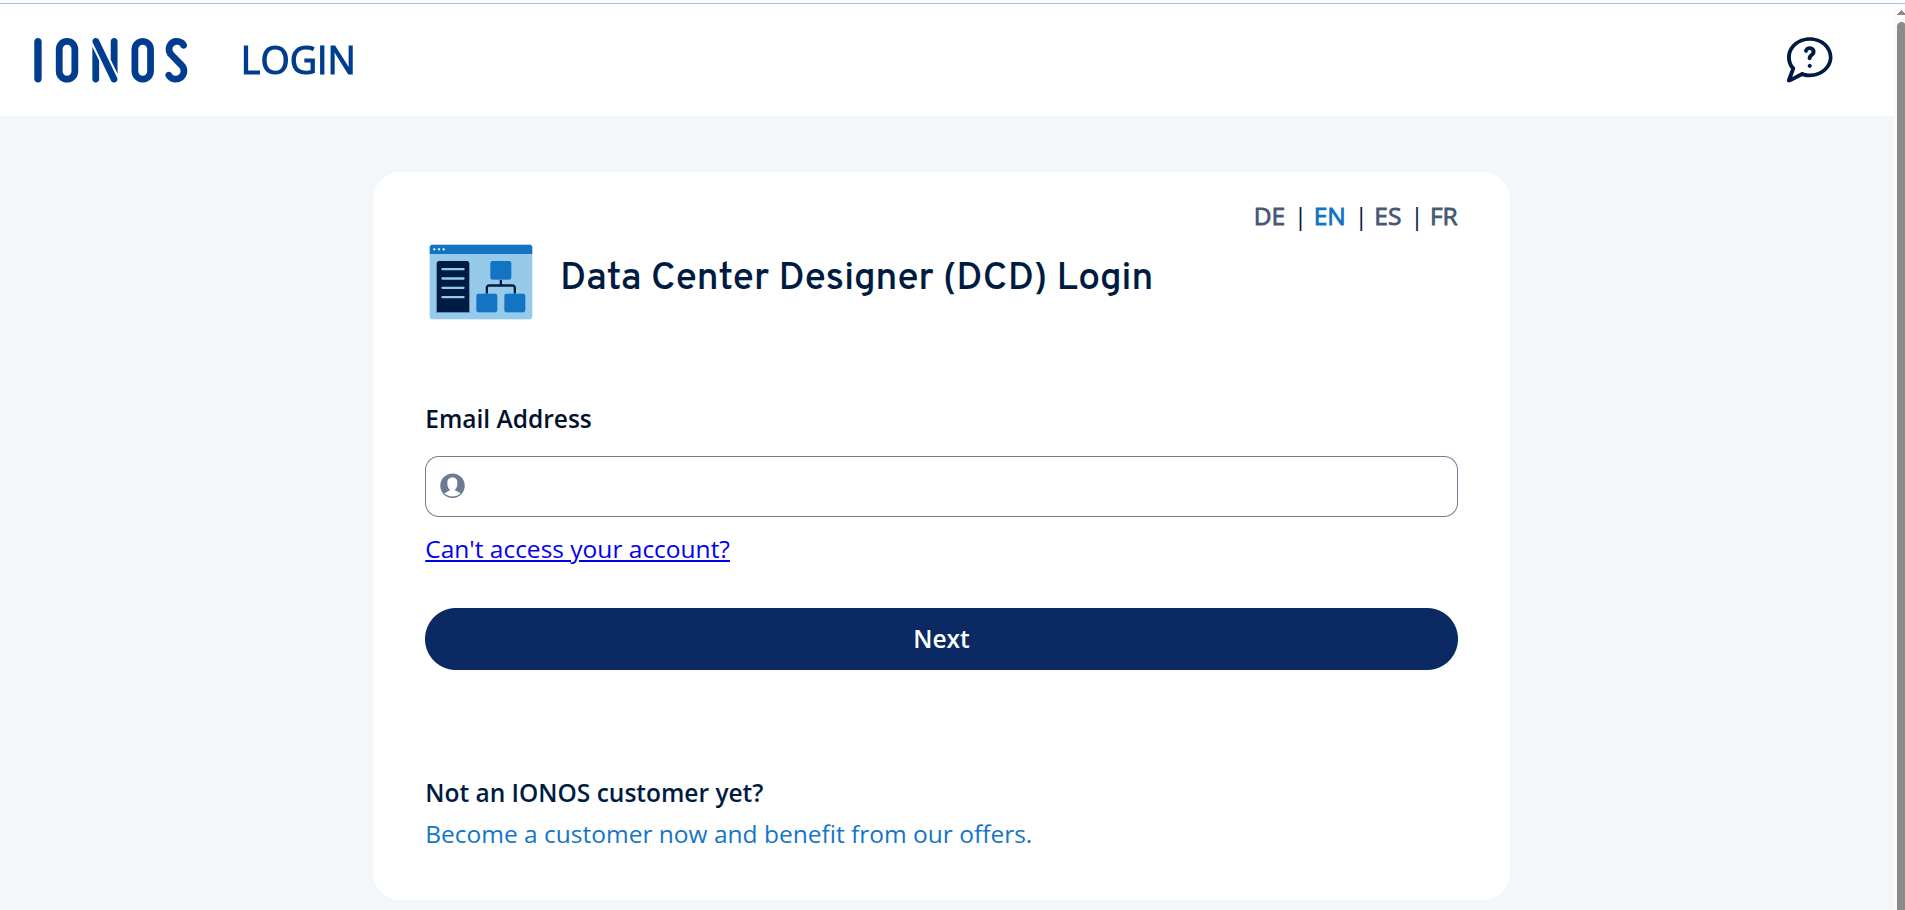
\includegraphics[width=10.5cm]{./imagenes/interfaz-InicioSesionDCD-1.png}
\caption*{Interfaz inicio sesión DCD IONOS Claud}
\end{center}
\end{figure}
Cuando se tenga cuenta solo hará falta añadir el correo en email address e iniciar sesión como es el estandar.
En el caso actual se debe dirigir a "\textit{Not an IONOS customer yet?}, dirgiendo este enlace a la web de creación de cuentas.

\begin{figure}[htb]
    \begin{center}
    \vspace*{0.3in}
    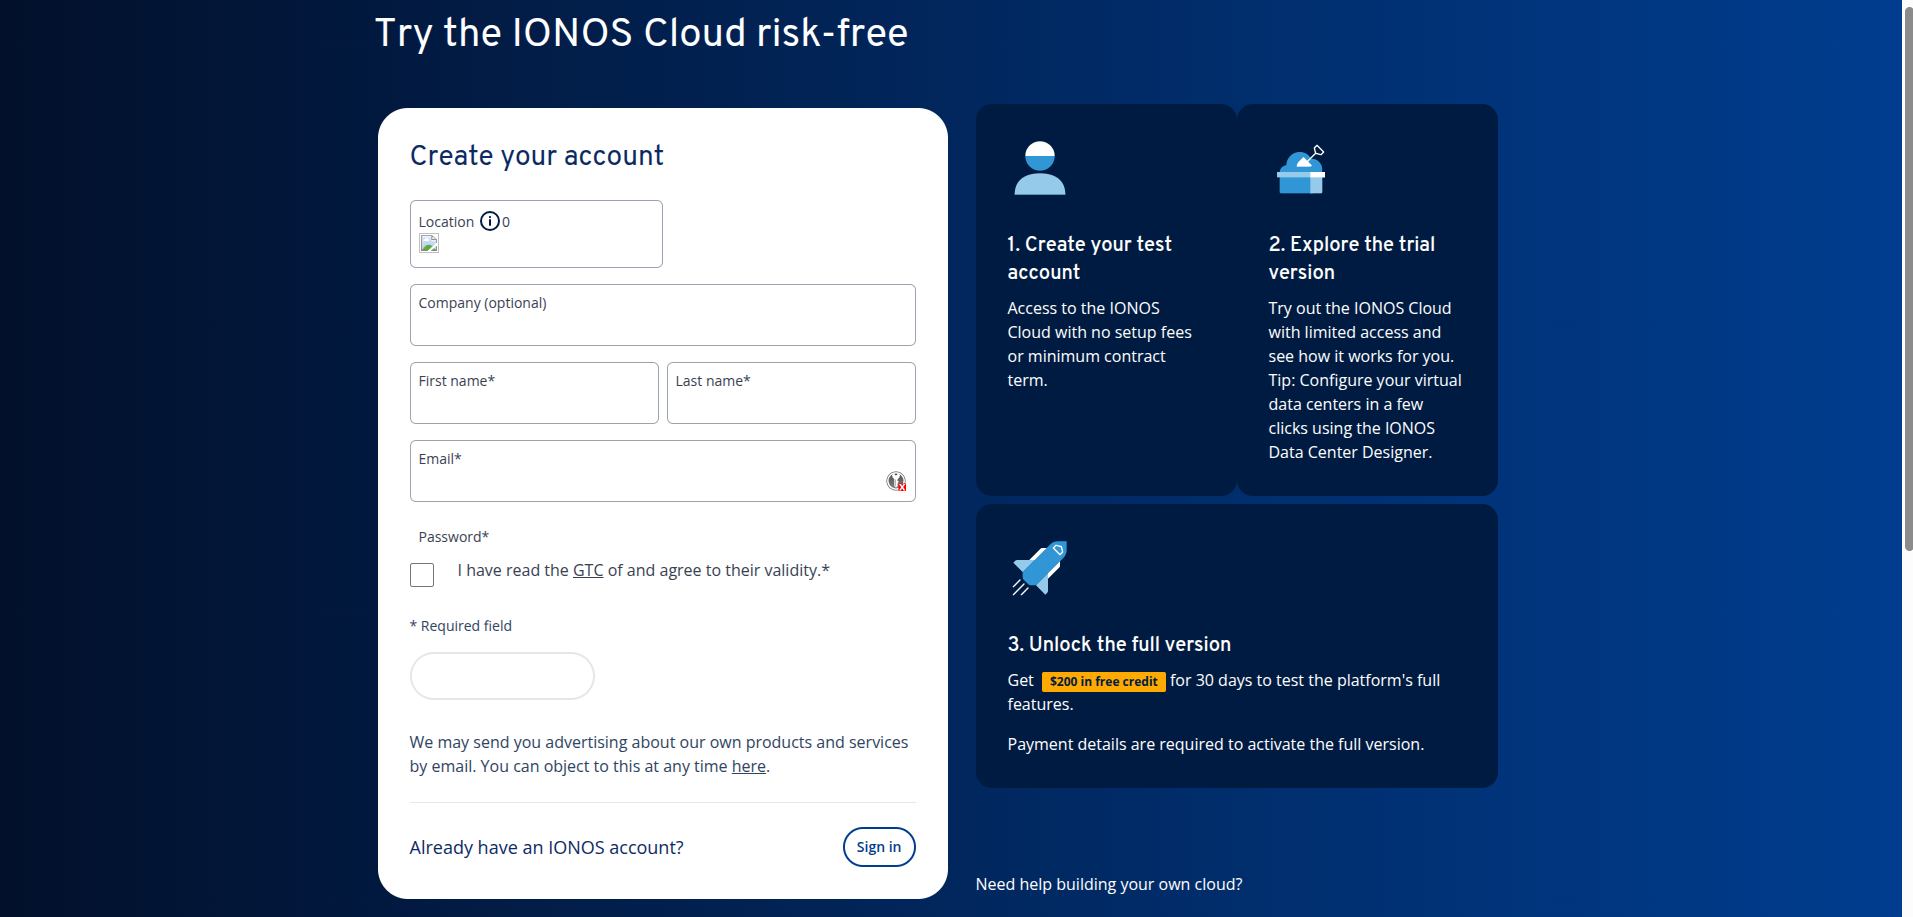
\includegraphics[width=10.5cm]{./imagenes/interfaz-InicioSesionDCD-2.png}
    \caption*{Crear cuenta IONOS Claud}
    \end{center}
\end{figure}

Como se puede ver en la imagen, lo unico que hay que hacer es añadir datos estandar y posteriormente aceptar sus políticas de privacidad.
Una vez creada la cuenta, se vuelve a la parte anterior y se inicia sesión con el correo al que se ha asociado la cuenta. Una ve iniciado se entrará en una pagina
similar a la mostrada actualmente. 

\begin{figure}[htb]
    \begin{center}
    \vspace*{0.3in}
    \includegraphics[width=12.5cm]{interfaz-DCD-1.png}
    \caption*{Iterfaz inicio DCD IONOS Claud}
    \end{center}
\end{figure}

Una vez dentro ya se habra creado el contrato y se tendrá la cuenta, completando el primer paso.

\section{Obtener token}
Una vez dentro de la interfaz, se debe pinchar en "\textit{MANAGEMENT}" donde se desplegará un menú en el que se deberá seleccionar \textit{"Token Manager"}.
\begin{figure}[htb]
    \begin{center}
    \vspace*{0.3in}
    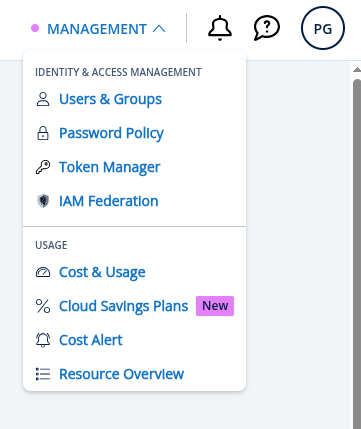
\includegraphics[width=4.5cm]{interfaz-DCD-3.png}
    \caption*{Barra de gestión del DCD}
    \end{center}
\end{figure}
Una vez dentro, es muy intuitivo como generar un token, se debe seleccionar la duración de validez del token, esta dependerá del uso que se quiera dar a dicho token. Una vez creado se debe almacenar correctamente dicho token, debido a que es información valiosa y se debe llevar acabo un protocolo te protección para este.
\begin{figure}[htb]
    \begin{center}
    \vspace*{0.3in}
    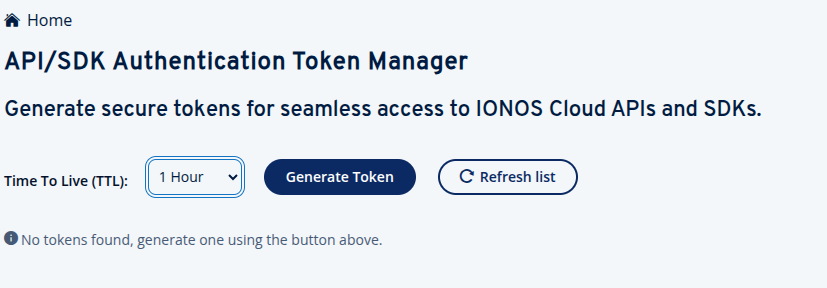
\includegraphics[width=10.5cm]{interfaz-DCD-tokens.png}
    \caption*{Interfaz de gestión de tokens}
    \end{center}
\end{figure}
\addtocontents{toc}{\protect\setcounter{tocdepth}{2}}

\newpage
\addcontentsline{toc}{chapter}{Anexo~3\quad{}Flujo de trabajo de la API Canary}
\addtocontents{toc}{\protect\setcounter{tocdepth}{-1}}
% ============================================
% ===== ANEXO 3: FLUJO DE TRABAJO API CANARY =====
% ============================================

\chapter{Flujo de trabajo de la API Canary}
\label{anexo:flujo-canary}

\subsection*{Diagrama}

\begin{figure}[h!]
    \centering
    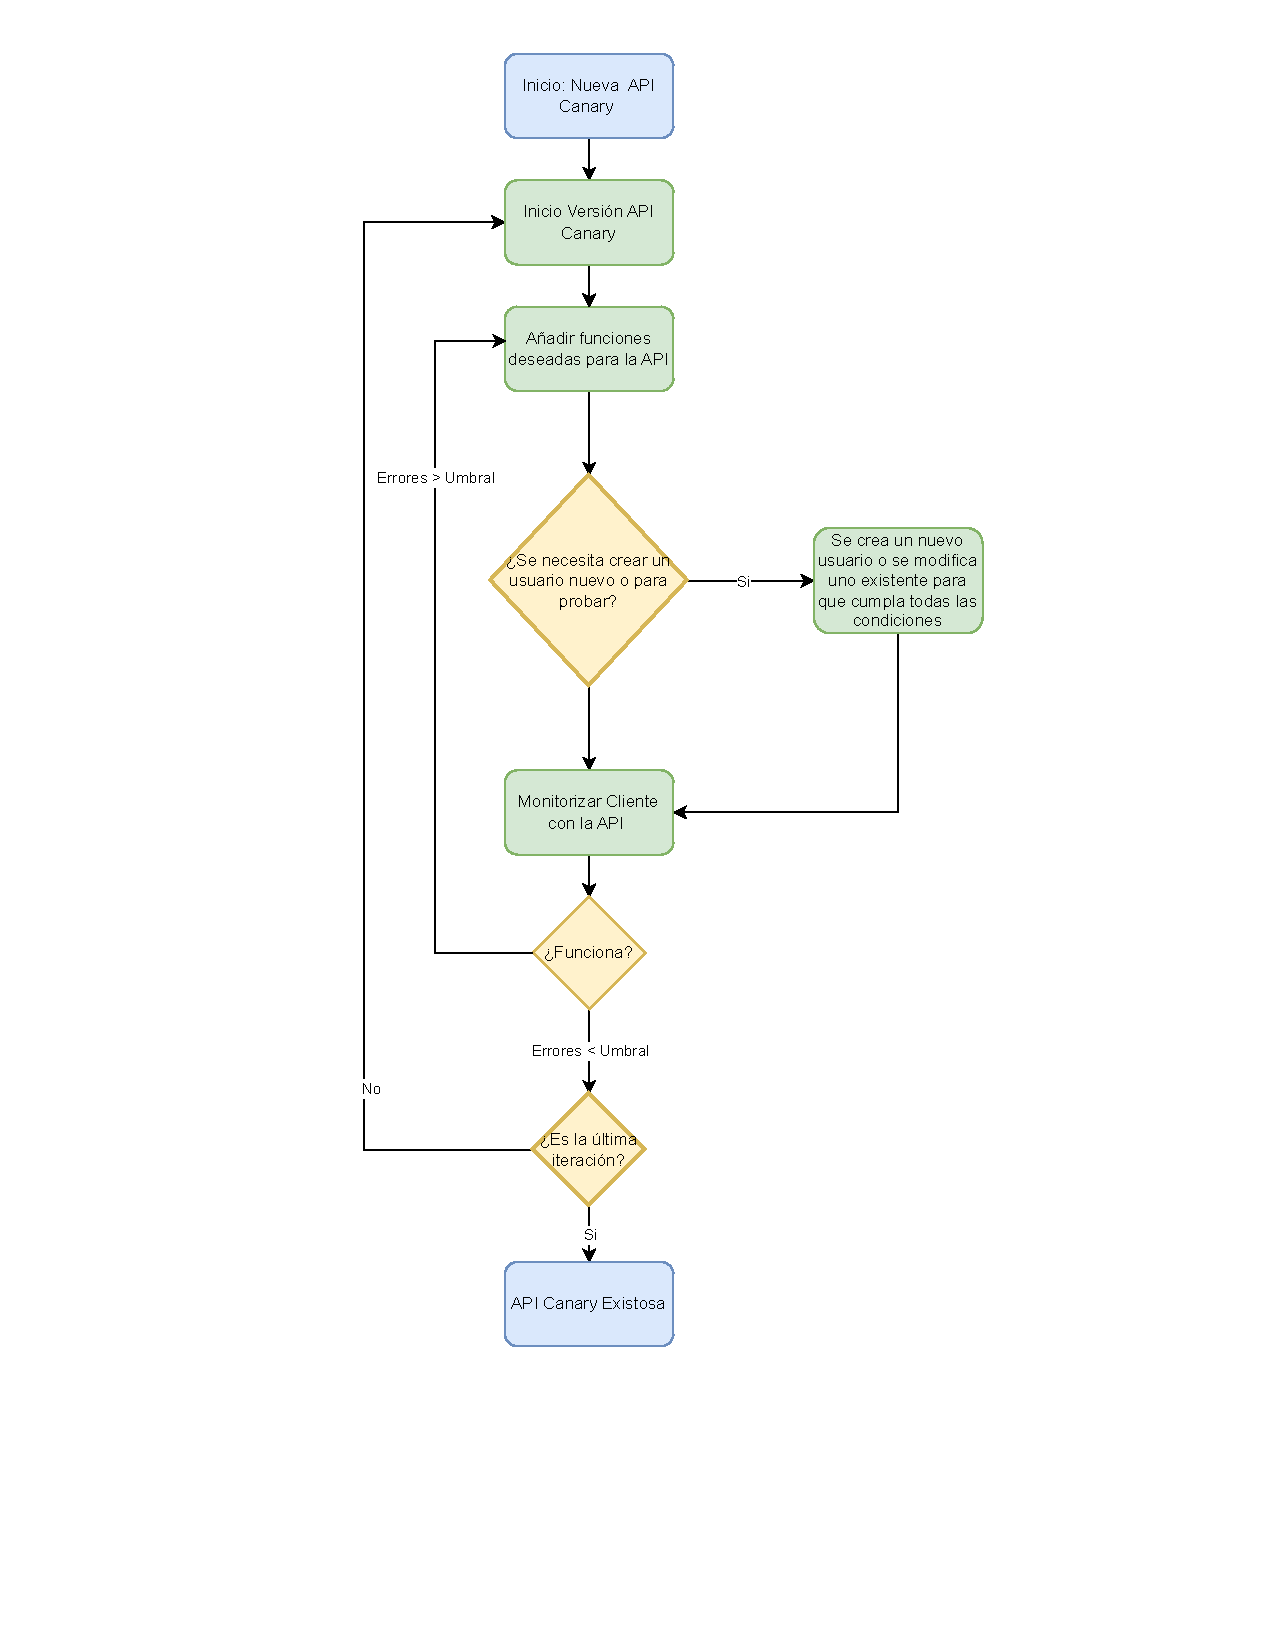
\includegraphics[width=0.9\textwidth]{archivos/flujo_API_Canary.drawio.pdf}
    \caption{Diagrama de flujo del proceso de despliegue Canary para APIs}
    \label{fig:canary-flow}
\end{figure}

\subsection*{Descripción del flujo}

\begin{enumerate}
    \item \textbf{Inicio: Nueva API Canary} --- Desarrollo de una nueva API de validación.

    \item \textbf{Inicio: Nueva versión de la API Canary} --- Inicio de una nueva iteración sobre la API existente, incorporando las funciones planificadas para esa fase.

    \item \textbf{Implementación de nuevas funciones} --- Se añaden las funcionalidades deseadas en el código de la API.

    \item \textbf{Comprobación del usuario de muestra} --- Se verifica que el usuario empleado para las pruebas dispone de todos los recursos necesarios. Si no es así, se ajusta su perfil o se crea uno nuevo que los incluya.

    \item \textbf{Monitorización de métricas} --- Análisis continuo de errores, latencia y otras métricas clave durante la ejecución.

    \item \textbf{Decisión basada en umbrales:}
          \begin{itemize}
              \item \textbf{Errores $<$ umbral} $\rightarrow$ La iteración se considera superada y se avanza a la siguiente fase.
              \item \textbf{Errores $>$ umbral} $\rightarrow$ Se realiza un \textit{rollback} automático a la versión estable anterior y se revisan los cambios para corregirlos.
          \end{itemize}

    \item \textbf{API Canary completada} --- Tras superar todas las fases, la API queda integrada y se programa su ejecución periódica automática.
\end{enumerate}





\addtocontents{toc}{\protect\setcounter{tocdepth}{2}}

% ===== BIBLIOGRAFÍA =====
\cleardoublepage
\printbibliography[title={Bibliografía}, heading=bibintoc]

\end{document}